\chapter{Results}
\label{chapter:results}
Instead of tying everything together at once, the project has been divided into five incremental phases. Being able to establish a working proof-of-concept for each step before adding on the extra complexity of the following step was a good strategy for determining which parts were working, and which parts needed to be worked on more.

The goals for each phase are described as follows:
\begin{enumerate}
    \item 2D optimization experiments
    \begin{itemize}[noitemsep]
        \item Build a simple, differentiable 2D rendering mechanism.
        \item It should support a set of basic parameterized transformations such as scaling, translation and rotation.
        \item Given a target image, it should be able to find the optimal transformation parameters to recreate the image using MSE loss.
    \end{itemize}
    
    Once a simple 2D baseline has been established, it can be extended to incorporate an actual CLIP-based loss function.
    \item 2D semantic experiments
    \begin{itemize}[noitemsep]
        \item Replace the MSE loss with a CLIP-based loss.
        \item It should be able to adequately optimize these transformation parameters wrt. a given text prompt.
    \end{itemize}

    Next, the 2D operations can be extended to 3D by using a different rendering mechanism. This brings the problem closer to the full NeRF-based pipeline, and introduces additional transformation parameters.
    \item 3D semantic experiments
    \begin{itemize}[noitemsep]
        \item Swap out the 2D rendering mechanism with a 3D rendering mechanism.
        \item Experiment with novel view augmentation (i.e. pass multiple rendered images from the scene to CLIP).
    \end{itemize}
    
    Before proceeding, it should be proven that the transformations for disentangled NeRFs work adequately. This is done using fixed transformation parameters (i.e. not semantically guided).
    \item Disentangled NeRFs
    \begin{itemize}[noitemsep]
        \item Successfully perform NeRF disentanglement
        \item Perform transformations on disentangled NeRFs
    \end{itemize}
\end{enumerate}

\section{2D optimization experiments}
\label{sec:2d-optimization}
% describe setup
The purpose of this phase is to explore the feasibility of optimizing a set of transformation parameters for a rendering mechanism with respect to an MSE loss function. Given a parameterized rendering mechanism $R(s)$, the loss function is defined as follows:
\begin{equation}
    \mathcal{L}(s) = || R(s) - R(s_{target}) ||^2_2
    \label{eq:mse_loss}
\end{equation}

% describe loss
The loss in eq. \ref{eq:mse_loss} can also be described as the MSE loss between the image rendered with the parameters $s$ and the target image, which was rendered with the parameters $s_{target}$. Thus, the objective is to find $s^* = s_{target}$, as this will have the lowest loss value.

% intro rendering mechanism
The PyTorch library kornia\footnote{\url{https://github.com/kornia/kornia}} was very useful for implementing the differentiable rendering mechanism - it contains a wide range of differentiable image operations, which made it quick and easy to build the renderers.

% intro mug rotation renderer
Initially, a renderer with a single parameter $s$ for controlling the rotation of a coffee cup was implemented. Instead of just clamping the parameter $s$ to a certain range (e.g. $[-180,180]$), a more gradient-preserving formulation was used for calculating the effective degrees of rotation: $rot(s) = \tanh(s)*180$. Thus, the operation is able to rotate the cup by degrees in the range $[-180, 180]$.

\begin{figure}[H]
    \centering
    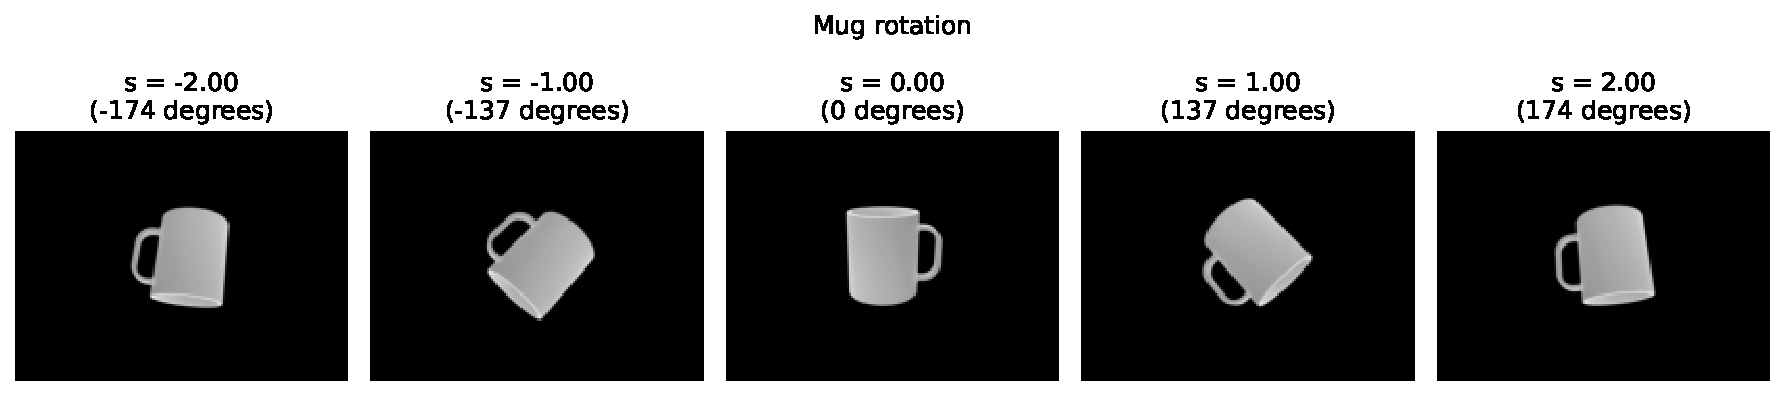
\includegraphics[width=1.0\textwidth]{figures/3_1-rotations.pdf}
    \caption{A sample of various $s$-values and the corresponding rendered images.}
    \label{fig:3_1-rotations}
\end{figure}

% intro rotation loss landscape
Setting $s_{target}= 0.0$ and computing the loss from eq. \ref{eq:mse_loss} for 100 $s$-values sampled in the range $[-2, 2]$ produced the results seen in figure \ref{fig:3_1-rotation-landscape}.

\begin{figure}[H]
    \centering
    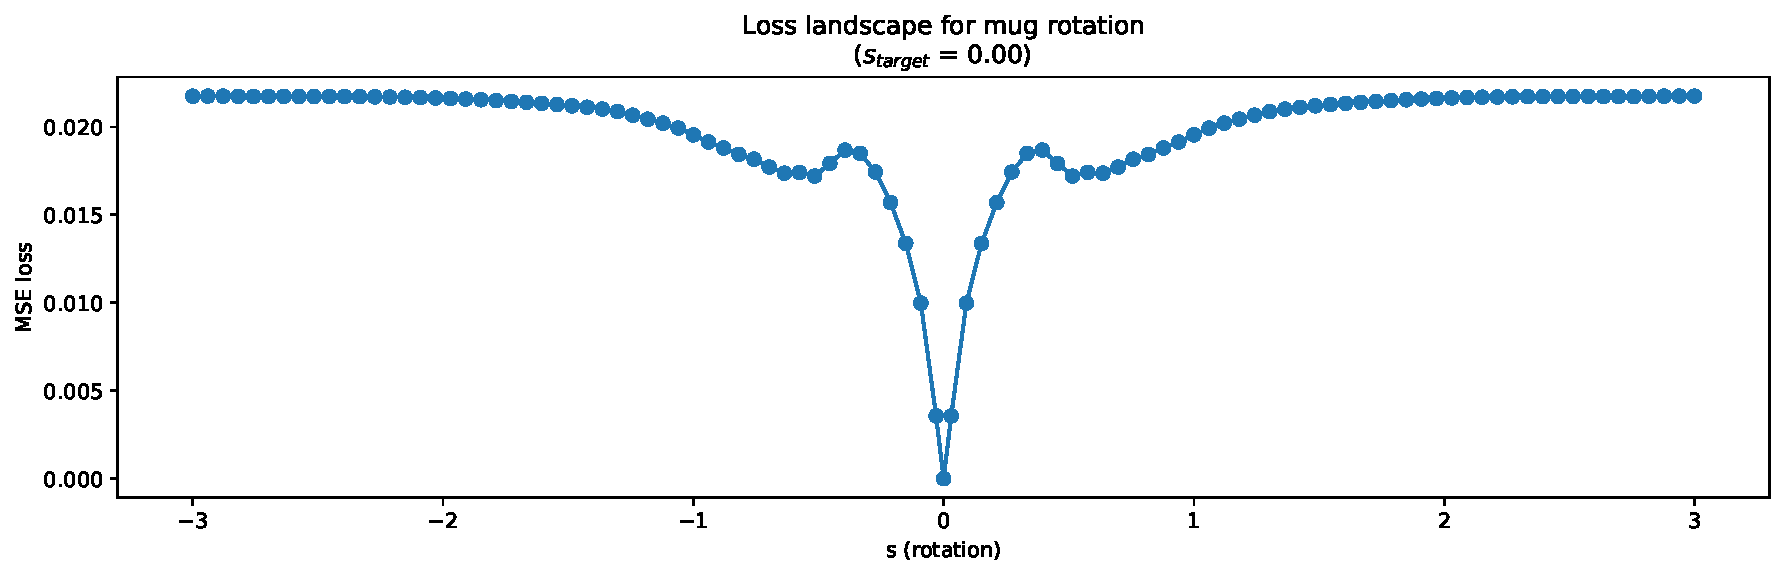
\includegraphics[width=1.0\textwidth]{figures/3_1-rotation-landscape.pdf}
    \caption{MSE loss landscape for mug rotation for 100 sampled $s$-values in the range $[-3,3]$}
    \label{fig:3_1-rotation-landscape}
\end{figure}
Figure \ref{fig:3_1-rotation-landscape} shows that the loss landscape is nonconvex. There is a clear global minimum around $s=0.0$, which is expected. It also shows two local minima on either side of the global minimum. Another observation to make is the fact that the boundary losses will become identical as $s\rightarrow \pm \infty$, since rotating by $\pm 180$ degrees will produce identical images.

% brute force sucks
The approach of evaluating many $s$-values within a given range (in our case $[-3,3]$) and simply returning the lowest value observed can be considered a brute force solution to the parameter optimization problem. In the simplified example, the strategy remains feasible, but it is important to note that the brute force search runs in exponential time. Imagine that the parameter count increased to $n=4$ (rotation, x-translation, y-translation scale), and the resolution (i.e. how many values to sample from each parameter range) remained $r=100$. The amount of evaluations required then becomes $r^n = 100^4 = 10^8$, which is a rather hefty amount. Time complexity becomes even more of an issue when the rendering mechanism is swapped out for more advanced mechanisms (e.g. NeRF), which are more expensive to run.

% intro gradient descent
Thus, a more elegant and efficient solution to the optimization problem is needed. A viable alternative could be gradient-based optimization methods. Recall that the rendering mechanisms are immediately differentiable thanks to kornia. This means that the gradient $\frac{\partial L}{\partial s}$ is available and can be used for gradient descent optimization.

A training loop for gradient descent was implemented using Adam with a learning rate of 0.05. The loop was run for 50 iterations for two different initial values for $s$: [-1.0, 2.0].

% rotation
\begin{figure}[H]
    \centering
    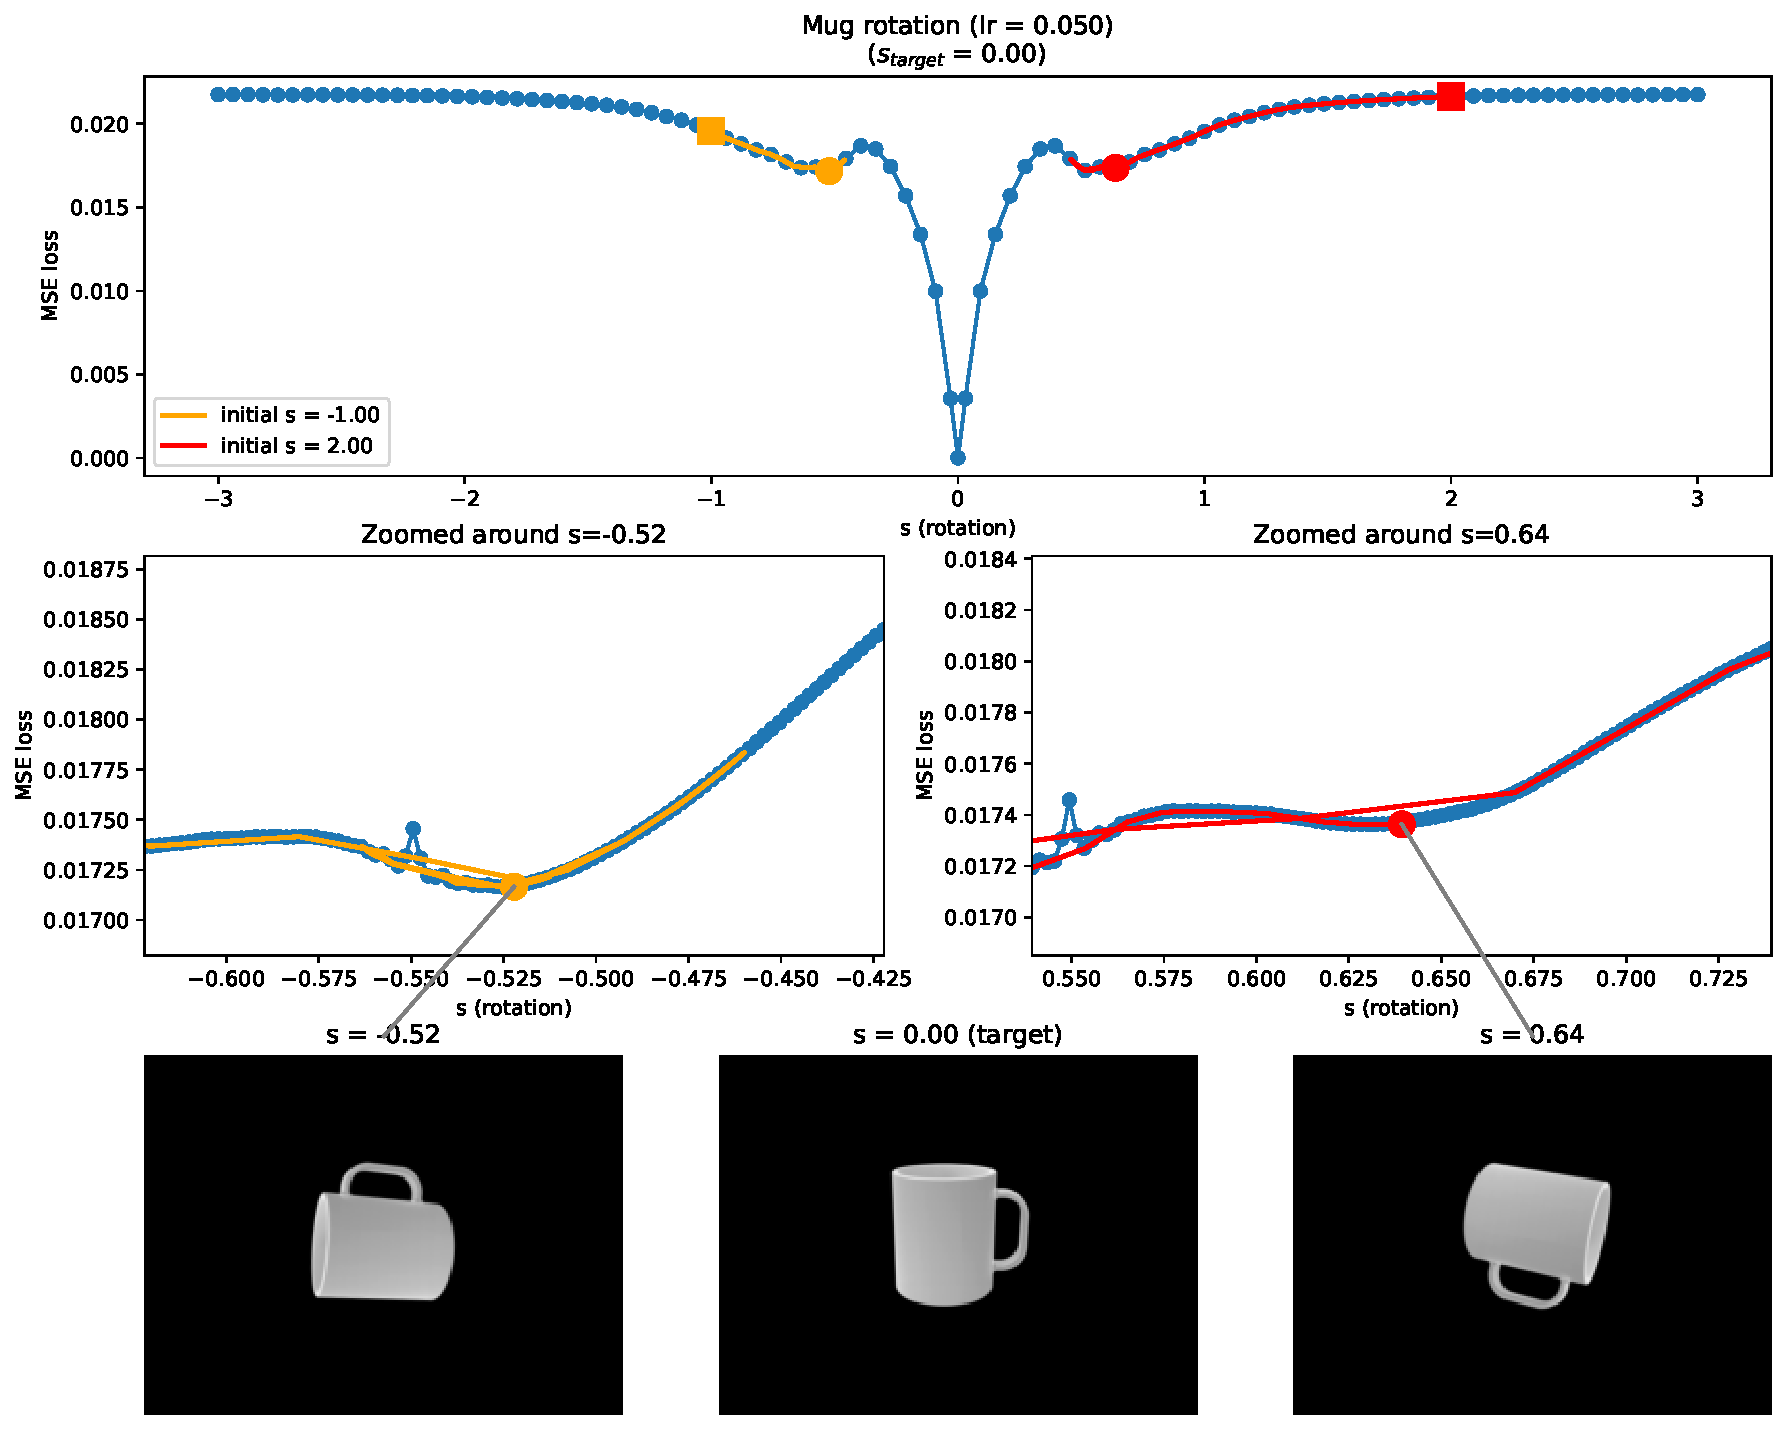
\includegraphics[width=1.0\textwidth]{figures/3_1-mse-gd-rotation-optimization.pdf}
    \caption{The first row shows the previous loss landscape overlaid with the gradient descent paths for two different starting points (the square marker is the starting point, the circle is the final point). The middle row shows two "zoomed in" views of the plot above. The bottom row shows the final solutions together with the target image.}
    \label{fig:3_1-mse-gd-optimization}
\end{figure}
From figure \ref{fig:3_1-mse-gd-optimization} it appears that the gradient descent procedure fails to find the global minimum at $s = s_{target} = 0.0$. For both starting points, the algorithm ends up in a local minimum. Also - it's not by chance that these two minima exist. They occur when the rotated cup is at a sort of "equilibrium point" at which the loss is improved equally when rotating the cup in either direction - i.e. a sort of ambiguity is at play here. This is the case when the rotated cup is perpendicular to the target cup.

Similar rendering mechanisms were made, which were respectively able to scale and x-translate the coffee cup instead. This produced the results seen in figure \ref{fig:3_1-other-transforms}.

% other transformations
\begin{figure}
    \centering
    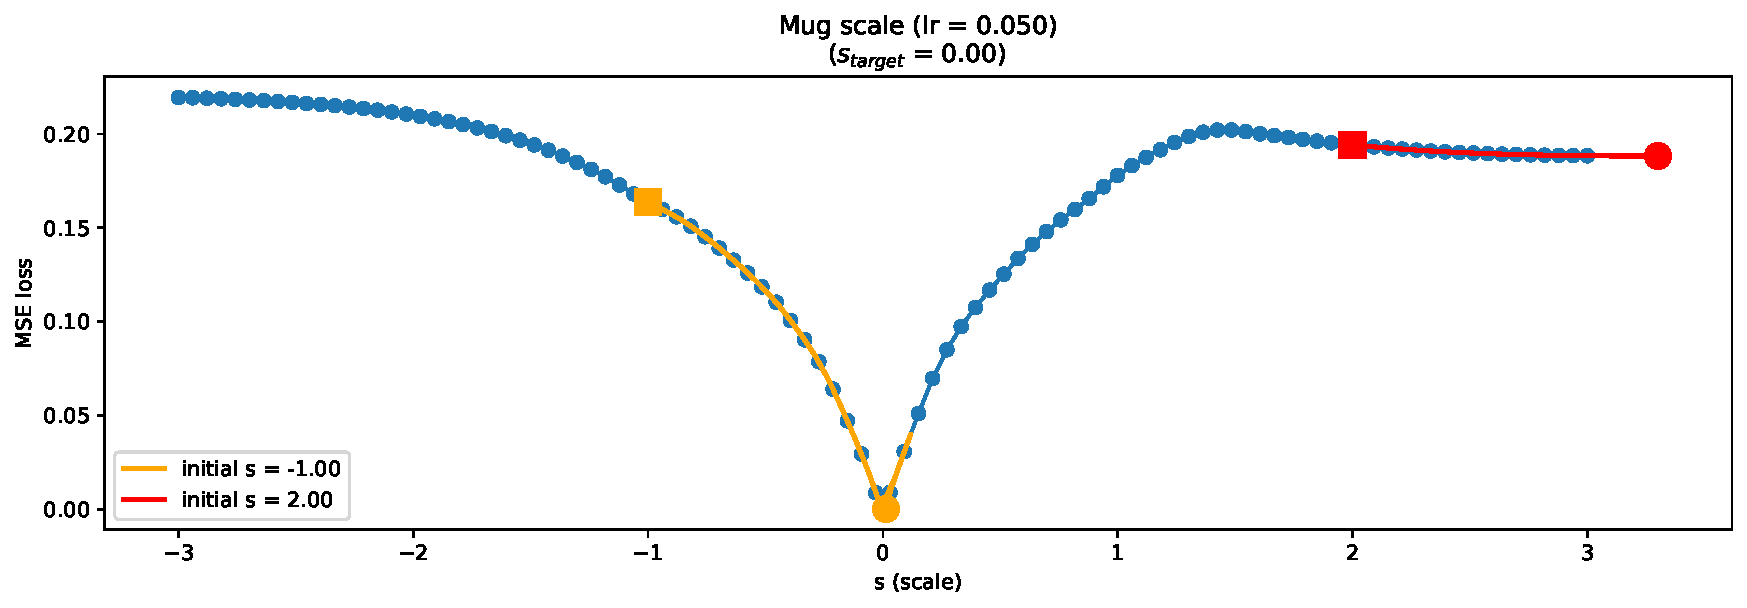
\includegraphics[width=1.0\textwidth]{figures/3_1-mse-gd-scale-optimization.pdf}
    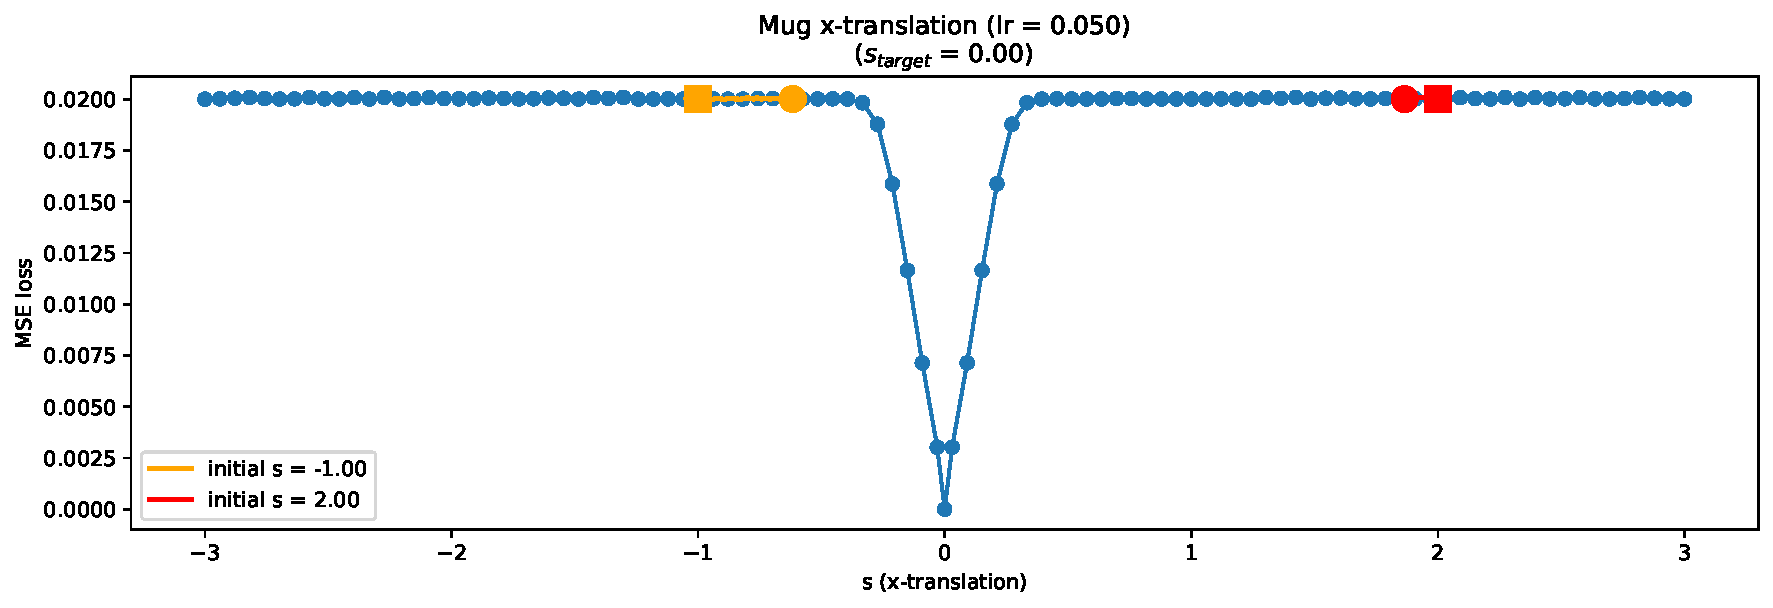
\includegraphics[width=1.0\textwidth]{figures/3_1-mse-gd-x-translation-optimization.pdf}
    \caption{Top row shows the loss landscape for the scaling renderer. Bottom row shows the loss landscape for the x-translating renderer.}
    \label{fig:3_1-other-transforms}
\end{figure}
Figure \ref{fig:3_1-other-transforms} shows that the issue with local minima also affected the other types of transformations. If the initial guess was sufficiently close to $s_{target}$, then gradient descent was able to find its way to the optimal solution. Otherwise, it could still get stuck in a local minimum

Also, it is quite interesting to see the "plateaus" for the x-translation loss landscape in figure \ref{fig:3_1-other-transforms}. The intuition behind this can be explained by a small example: Imagine the target cup being far over on the right side of the image. Now, for a cup on the left side of the image, which has no overlap at all with the target cup on the right, the loss will remain the same when stepping either left or right. This will be the case until the cups start overlapping, at which point the "valley" in the loss landscape starts to appear. This kind of fundamental ambiguity is what makes the optimization problem difficult to solve with gradients.

Additional experiments were performed in hopes of improving the gradient descent approach. Switching the MSE loss with an L1 loss made no real difference. Switching the optimization algorithm from Adam to RMSprop, Adagrad, SGD did not help much either. The most significant knobs to tweak were the starting points and the learning rate. If adjusted correctly, the learning rate can help gradient descent escape the local minima. However, if the learning rate was too big, the algorithm ended up "overshooting" and escaping the global minimum. This can be seen in figure \ref{fig:3_1-lr-experiment}.

\begin{figure}[H]
    \centering
    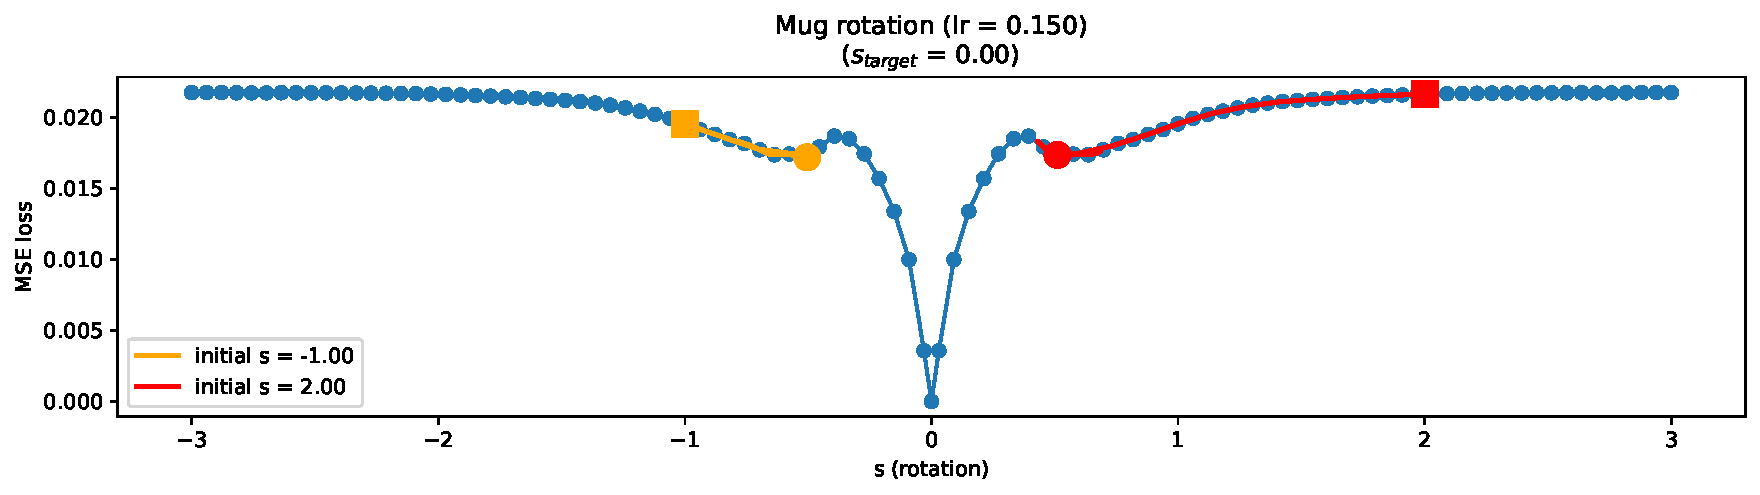
\includegraphics[width=1.0\textwidth]{figures/3_1-mse-gd-rotation-optimization-lr0.15.pdf}
    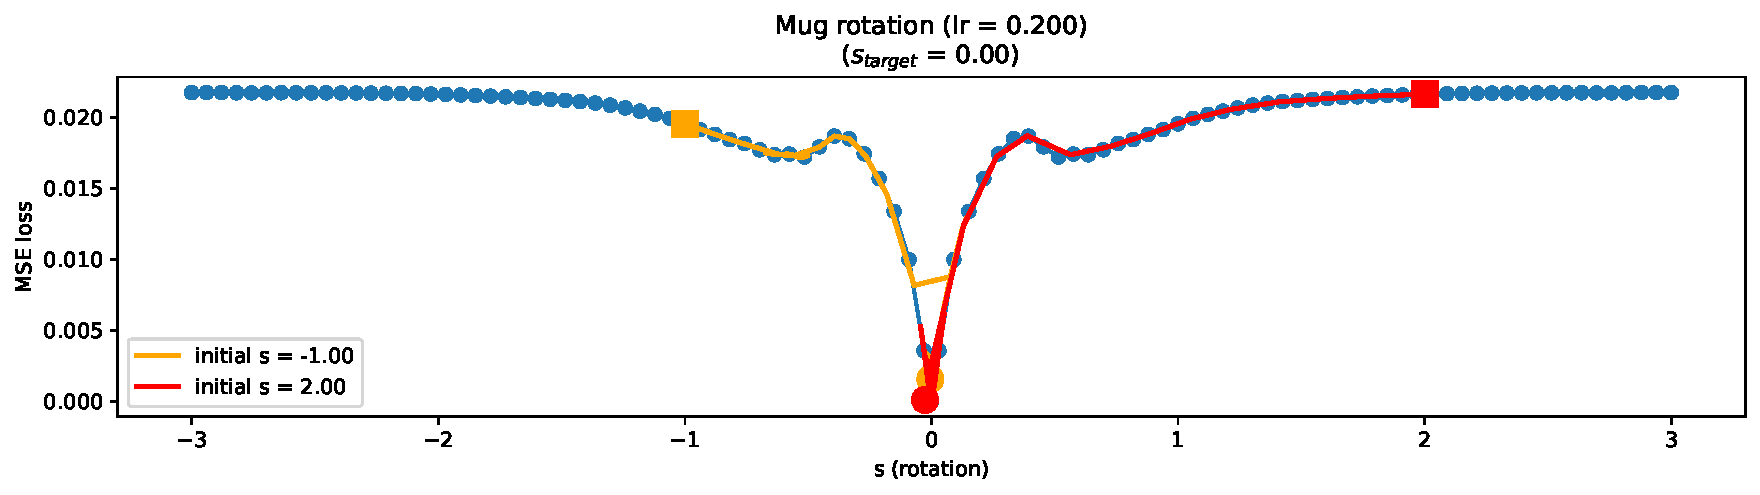
\includegraphics[width=1.0\textwidth]{figures/3_1-mse-gd-rotation-optimization-lr0.20.pdf}
    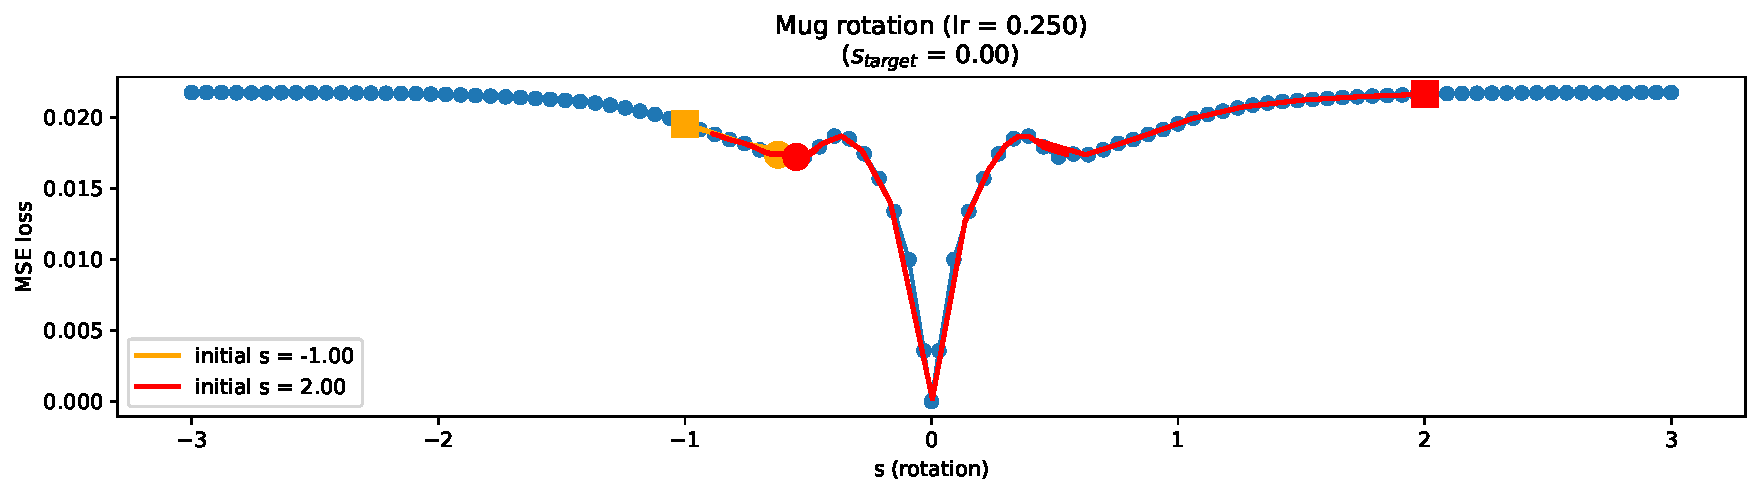
\includegraphics[width=1.0\textwidth]{figures/3_1-mse-gd-rotation-optimization-lr0.25.pdf}
    \caption{Gradient descent solutions for three different learning rates. The optimizer was Adam, and the iteration count was 50. The squares indicate starting points for gradient descent. The circles denote ending points.}
    \label{fig:3_1-lr-experiment}
\end{figure}


% intro global optimizers
Next, it's time to see how gradient-free optimization techniques perform on the task. For this, several algorithms from scipy\footnote{\url{https://docs.scipy.org/doc/scipy/reference/optimize.html}} were experimented with. Specifically, the following collection of methods: [basinhopping, differential\_evolution, dual\_annealing]. This produced the results seen in figure \ref{fig:3_1-global-optimizers}.

% global optimizer comparison
\begin{figure}[H]
    \centering
    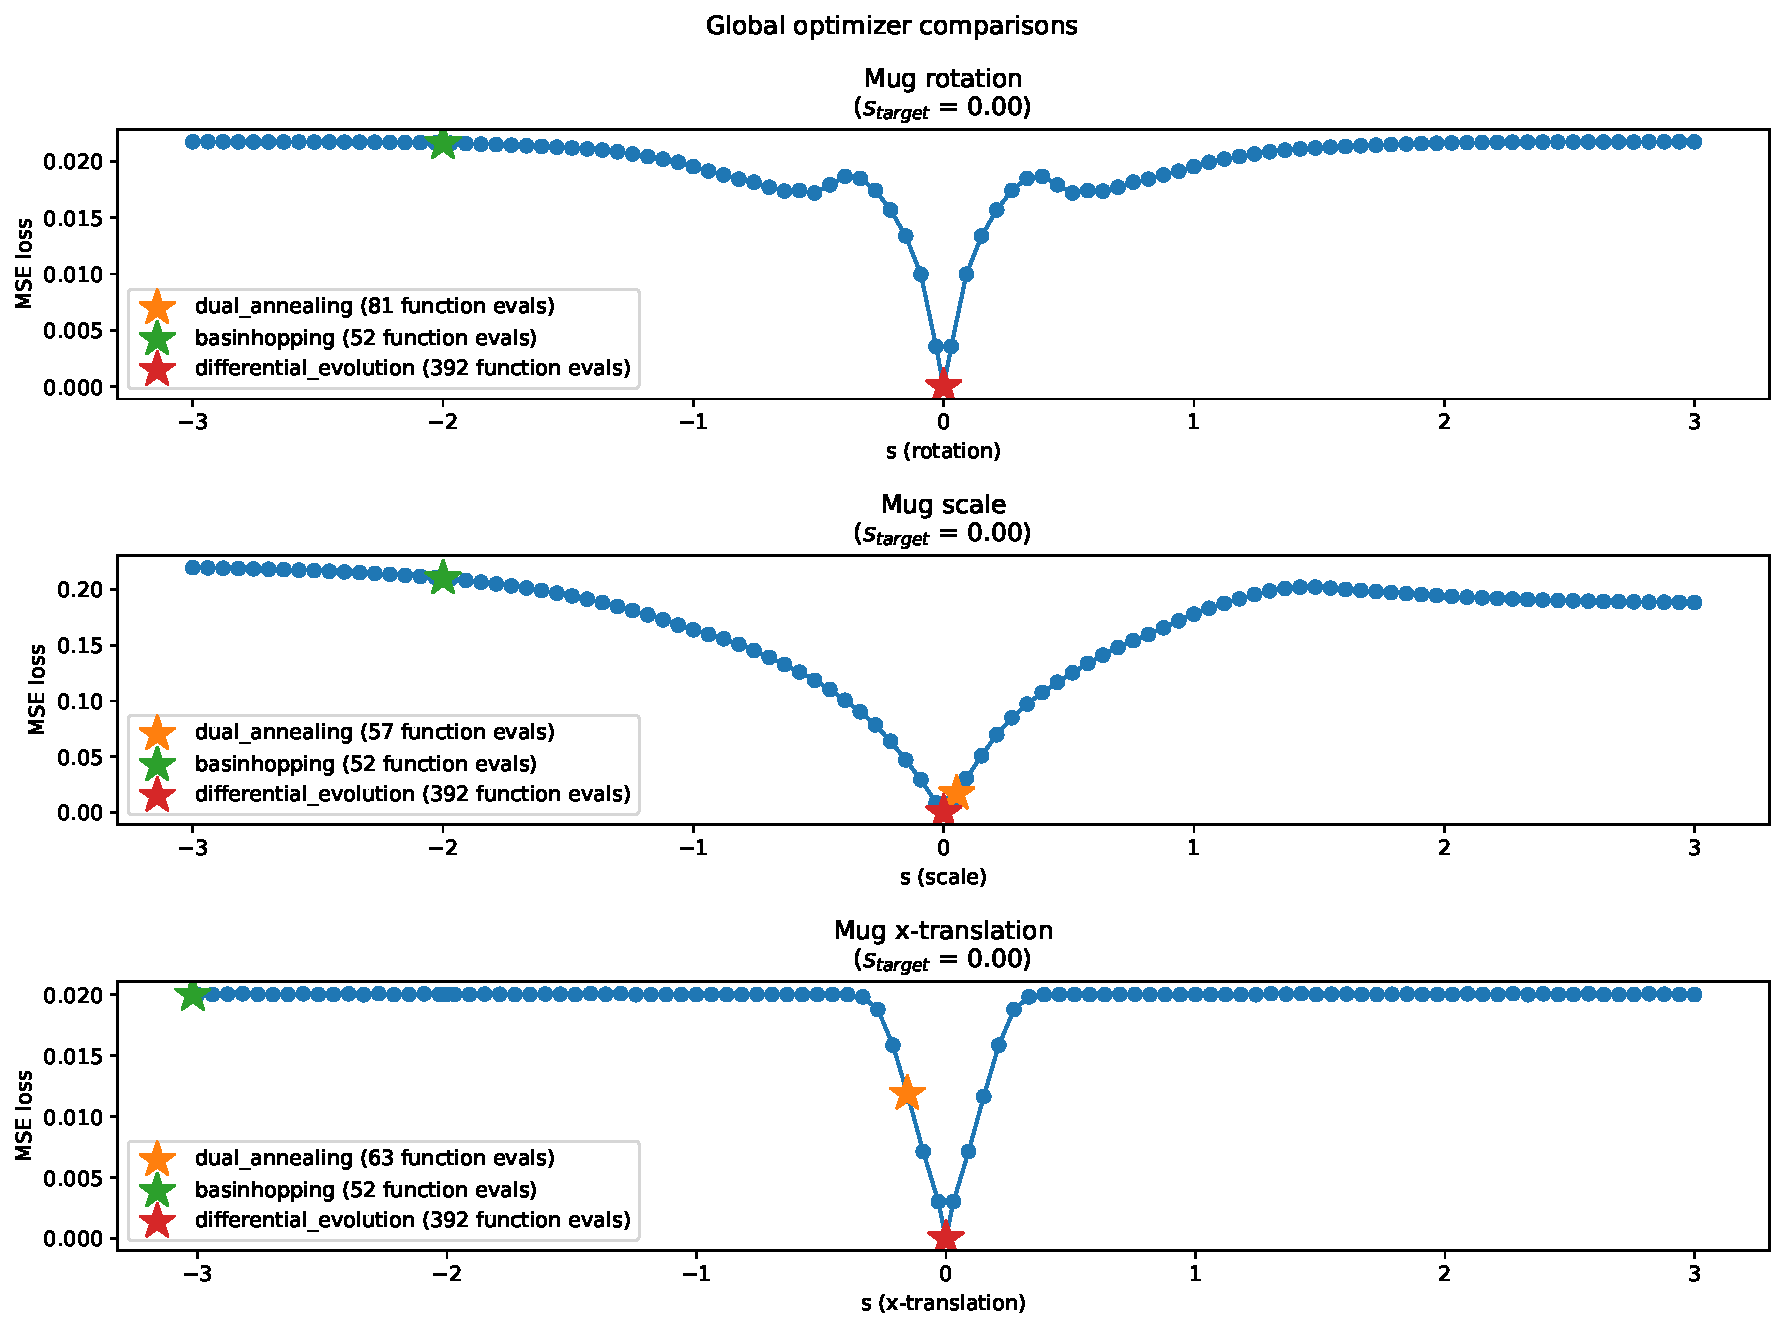
\includegraphics[width=1.0\textwidth]{figures/3_1-global-optimizers.pdf}
    \caption{Comparison of global optimization methods. Each row corresponds to a loss landscape for a certain transformation (respectively rotation, scale, and x-translation). The colored stars correspond to the final solutions obtained from the methods. The legend also denotes the amount of function evaluations performed during optimization.}
    \label{fig:3_1-global-optimizers}
\end{figure}
Figure \ref{fig:3_1-global-optimizers} shows a comparison of the different global optimization methods. When comparing the different optimization methods, it seemed like dual\_annealing had a good balance between speed (i.e. function evaluation count) and quality.

% subchapter recap
To summarize the findings of this subchapter:
\begin{itemize}[noitemsep]
    \item Even for the relatively simple MSE loss, the landscape is still non-convex due to the fundamental ambiguities described. Thus, there will be local minima and plateaus that can be challenging to optimize around.

    \item While it's not impossible for gradient descent to find the optimal solution, it usually requires a considerable amount of hyperparameter tweaking (e.g. optimizer, learning rate, initial guesses, etc.) to do so reliably.
    
    \item Gradient-free global optimization methods can be used as a backup when gradient descent fails. These are usually more expensive than gradient descent in terms of render evaluations, but they aren't quite susceptible to the same issues as gradient descent. Amongst the methods that were experimented with, dual\_annealing seemed to perform best.
\end{itemize}

\section{2D semantic experiments}
\label{sec:2d-semantic}
% subchapter intro
To establish the viability of semantically guided volumetric manipulations, it needs to be proven that CLIP is able to understand the visual effects of the transformations (e.g. scale, translation, rotation). Fortunately, OpenAI has published pre-trained versions of CLIP that are readily available\footnote{\url{https://github.com/openai/CLIP}}. Initially, the chosen CLIP model version is "ViT-L/14". The model is first loaded to the CPU and subsequently moved to the GPU in order to run using 32-bit floating point values (rather than the default optimized 16-bit floating point values).

% intro loss
The image rendering mechanisms from the previous subchapter were reused. However, the loss function was modified. Instead of using the MSE loss between the candidate image and a target image, the loss was now formulated as the negative CLIP similarity between the candidate image and a target text prompt. Formally, it can be formulated as follows:
\begin{equation}
    \mathcal{L}(s) = -E(R(s)) \cdot E(text\ prompt)
    \label{eq:clip_loss}
\end{equation}
In addition to the rendering mechanism $R(s)$ (which was also present in the previous subchapter), there is now $E(...)$, which denotes the CLIP encoder (used synonymously for image and text inputs), and $text\ prompt$, which denotes the given text prompt (i.e. a constant).

% simple scene
First, it might be insightful to see how a few example text prompts relate to the rendered images. For this example, the scaling renderer was used. The following two text prompts were used: ["a tiny coffee mug with no background", "a medium coffee mug with no background", "a huge coffee mug with no background"]. 100 $s$-values were sampled in the range $[-2,2]$. This produced the results seen in figure \ref{fig:3_2-scale-optimal-images}.
\begin{figure}[H]
    \centering
    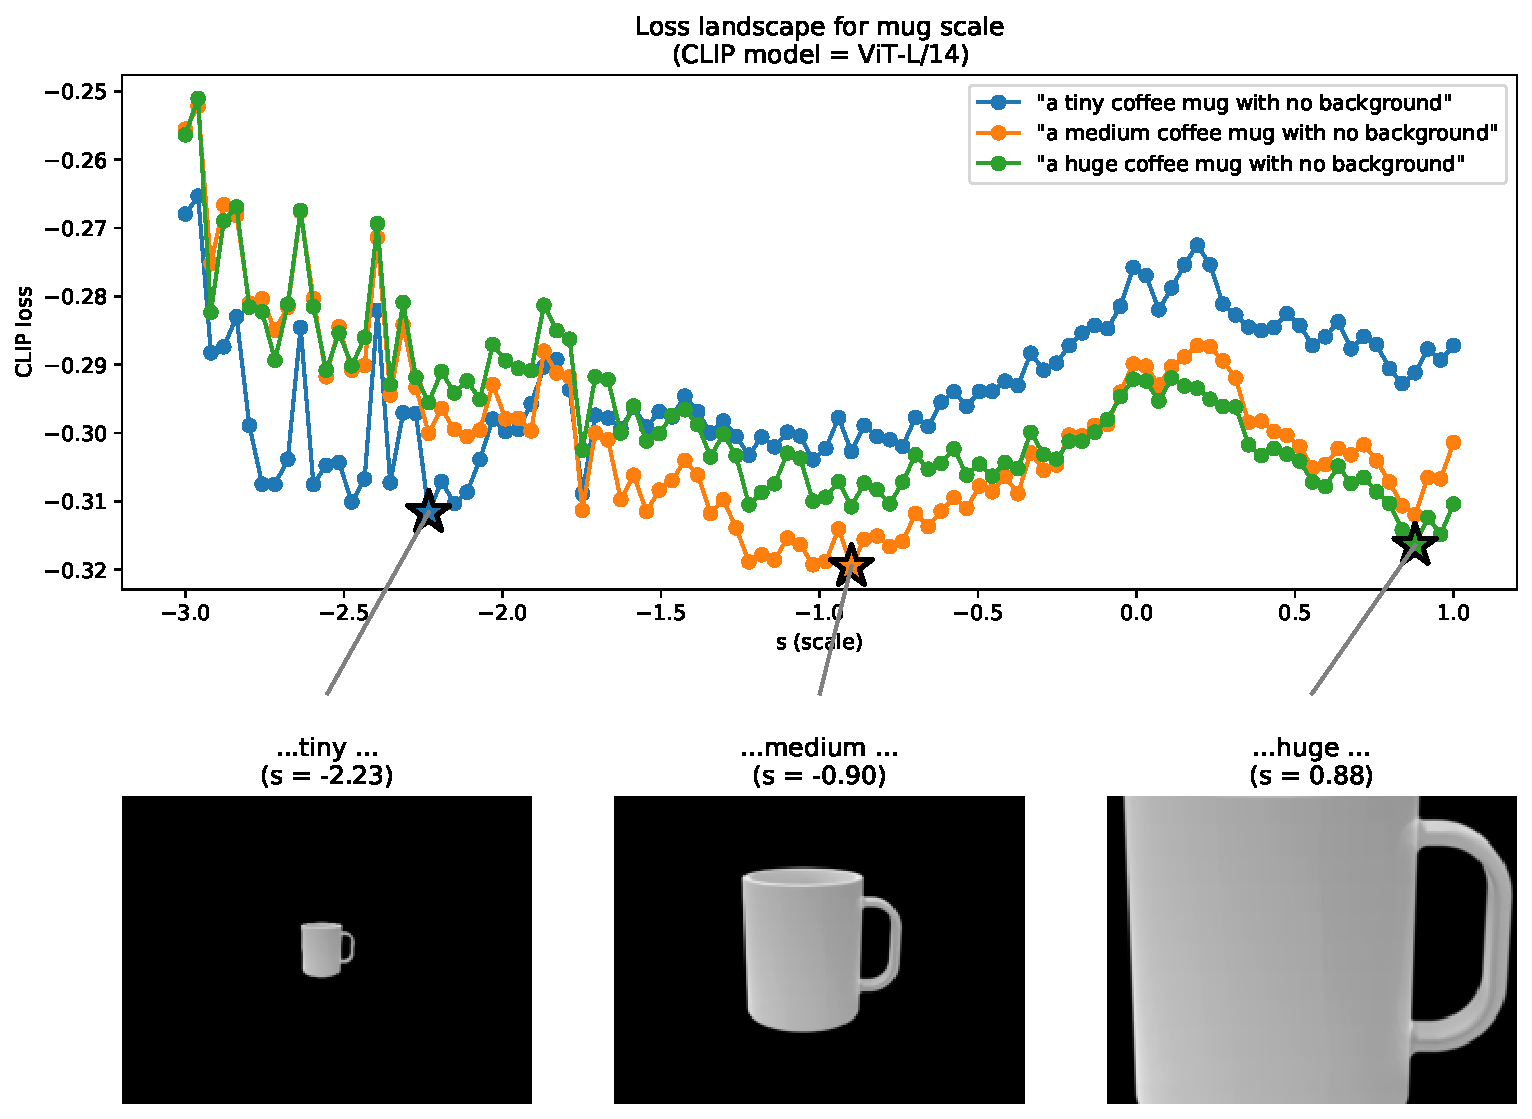
\includegraphics[width=1.0\textwidth]{figures/3_2-scale-optimal-images.pdf}
    \caption{Top row shows the CLIP loss landscape for the different text prompts overlaid with star markers that denote the corresponding minimum. Bottom row shows the resulting images rendered at the various minima.}
    \label{fig:3_2-scale-optimal-images}
\end{figure}
Figure \ref{fig:3_2-scale-optimal-images} demonstrates that CLIP has some understanding of scale-related adjectives in the context of scaling a mug with no background. However, the loss landscapes appear to be much noisier than the MSE loss landscapes seen in the previous subchapter, which could make it difficult for gradient descent to work effectively.


% complex scenes
The mug x-translation renderer was extended to also include a background image of an office (which is actually from a popular NeRF dataset). The idea is to gauge how well CLIP understands an image of a more complex image with several objects present. The text prompts were also changed to ["a coffee mug on the floor of an office", "a coffee mug on a table in an office"]. This produced the results seen in figure \ref{fig:3_2-room-translation-optimal-images}.
\begin{figure}[H]
    \centering
    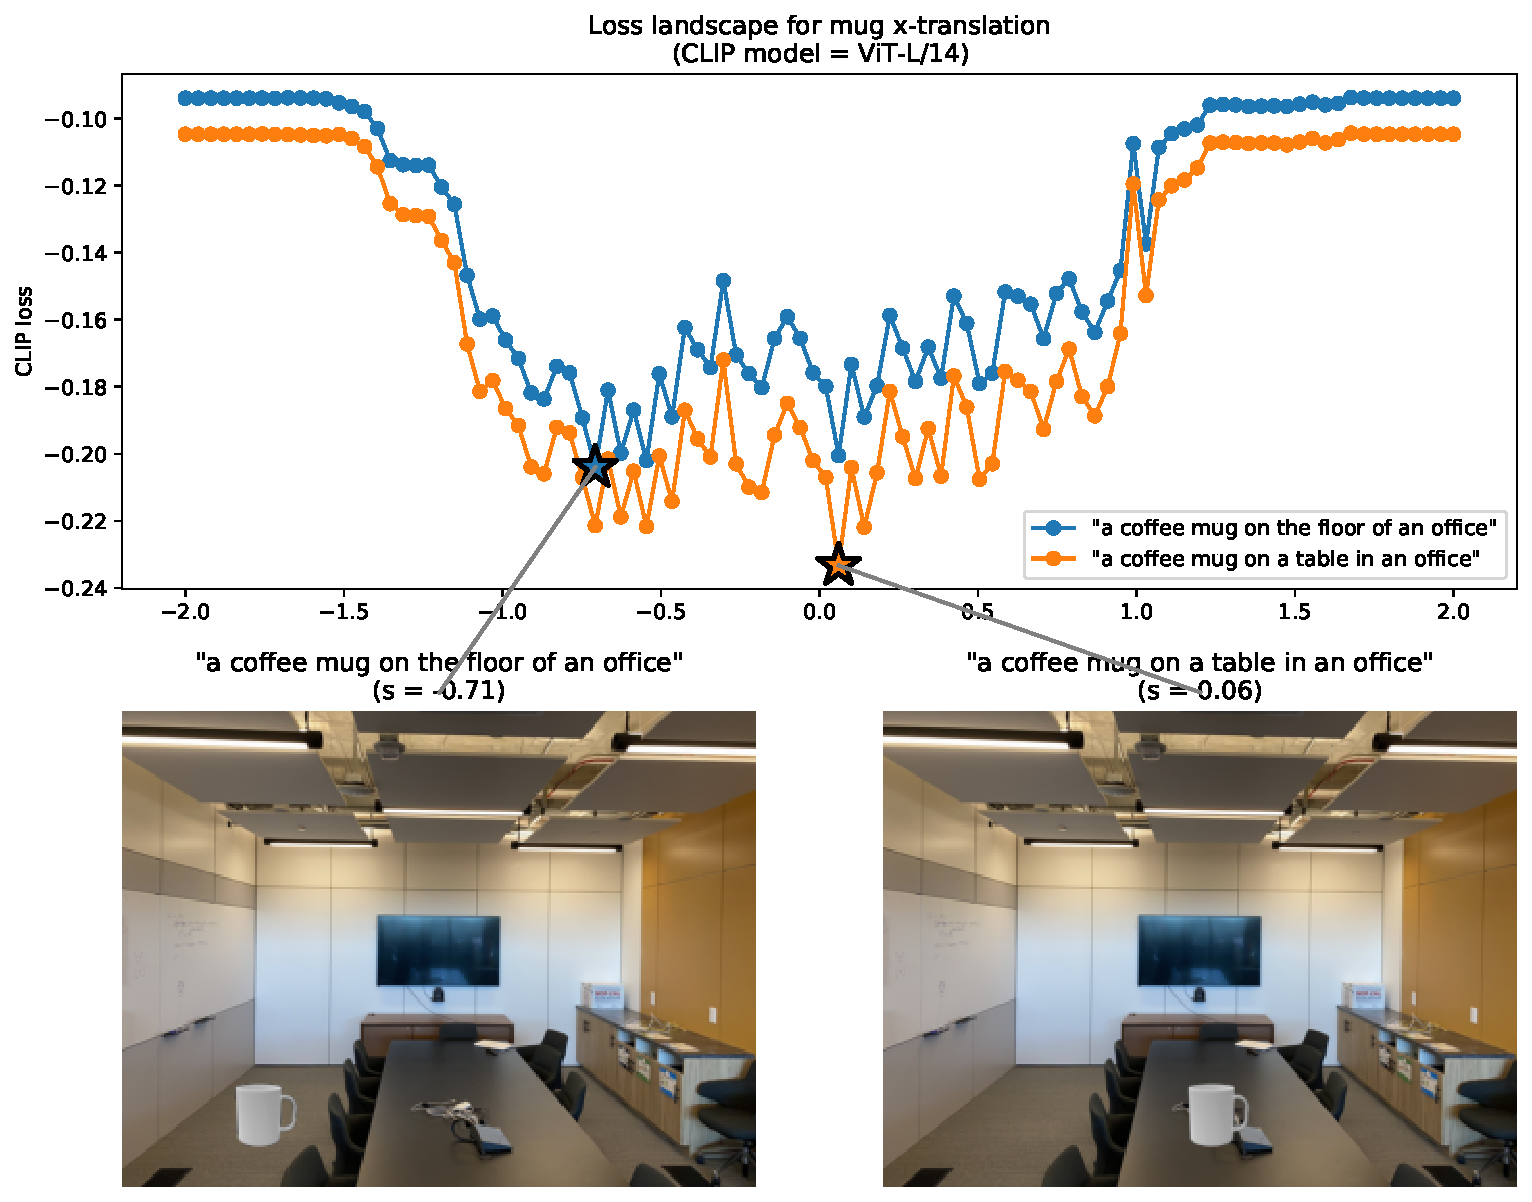
\includegraphics[width=1.0\textwidth]{figures/3_2-room-translation-optimal-images.pdf}
    \caption{Top row shows the CLIP loss landscape for the different text prompts overlaid with star markers that denote the corresponding minimum. Bottom row shows the resulting images for the various minima.}
    \label{fig:3_2-room-translation-optimal-images}
\end{figure}
Figure \ref{fig:3_2-room-translation-optimal-images} shows loss landscapes that are observably even noisier than the ones seen in figure \ref{fig:3_2-scale-optimal-images}. Despite the noise, the  minimum for the prompt "... on the floor of an office" correctly places the mug on the floor to the left, and the minimum for the prompt "... on a table in an office" correctly places the mug center on the table.

% zoomed in loss landscape
Recall that the loss landscapes have been plotted at a granularity of $N=100$ points in the range $[-2,2]$ for the parameter $s$. Perhaps "zooming in" and plotting the landscape at a different scale (i.e. finer resolution) could provide additional insight on how the landscape behaves. The 
\begin{figure}[H]
    \centering
    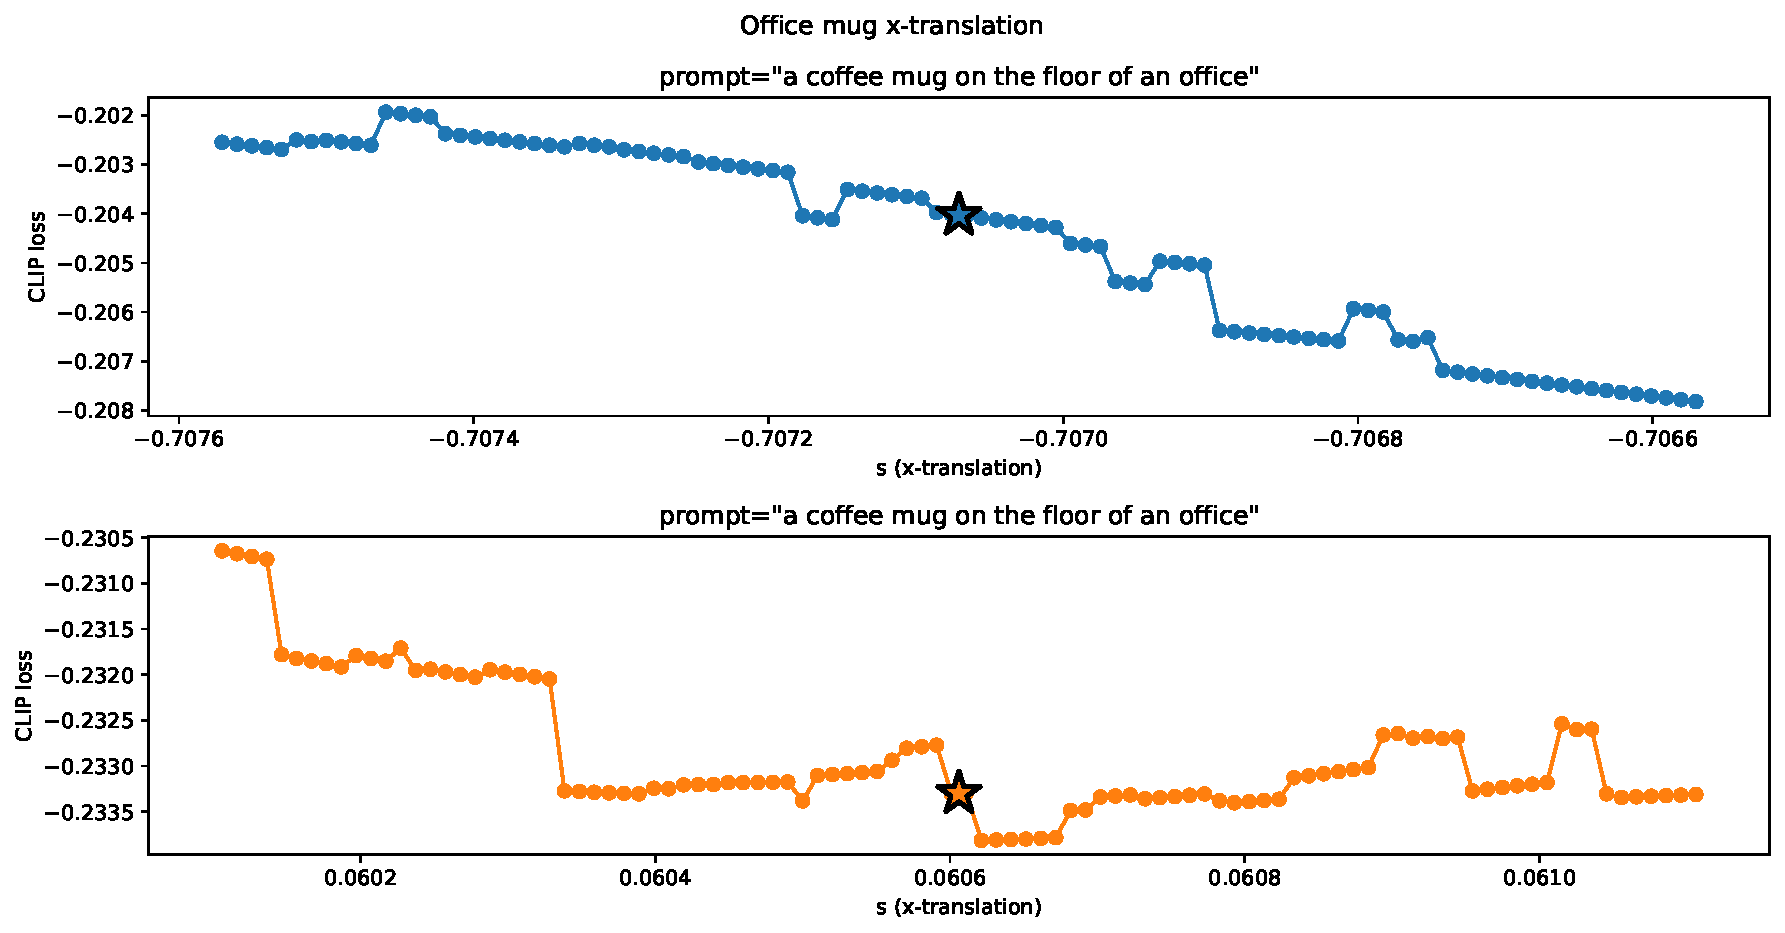
\includegraphics[width=1.0\textwidth]{figures/3_2-room-translation-optimal-images-zoomed.pdf}
    \caption{Zoomed in loss landscape for the example with mug x-translation in an office environment.}
    \label{fig:3_2-scale-optimal-images-zoomed}
\end{figure}
Figure \ref{fig:3_2-scale-optimal-images-zoomed} shows that the previously marked minima are in fact not the true global minima. Sampling the loss landscape at a higher resolution shows that there exists even better values for $s$. Another interesting detail is the fact that a minuscule change in $s$, which a human likely wouldn't notice, leads to a significant change in CLIP loss. This shows that the loss landscape is highly sensitive to $s$.

% basic shitty gradient descent
Ignoring the noisy loss landscape for now, it's time to see how well gradient descent works for optimization. A training loop was set up together with a cosine annealing learning rate scheduler. Running the loop for 300 iterations with an initial learning rate of $0.1$ produced the results seen in figure \ref{fig:3_2-room-vanilla-gd}.

\begin{figure}[H]
    \centering
    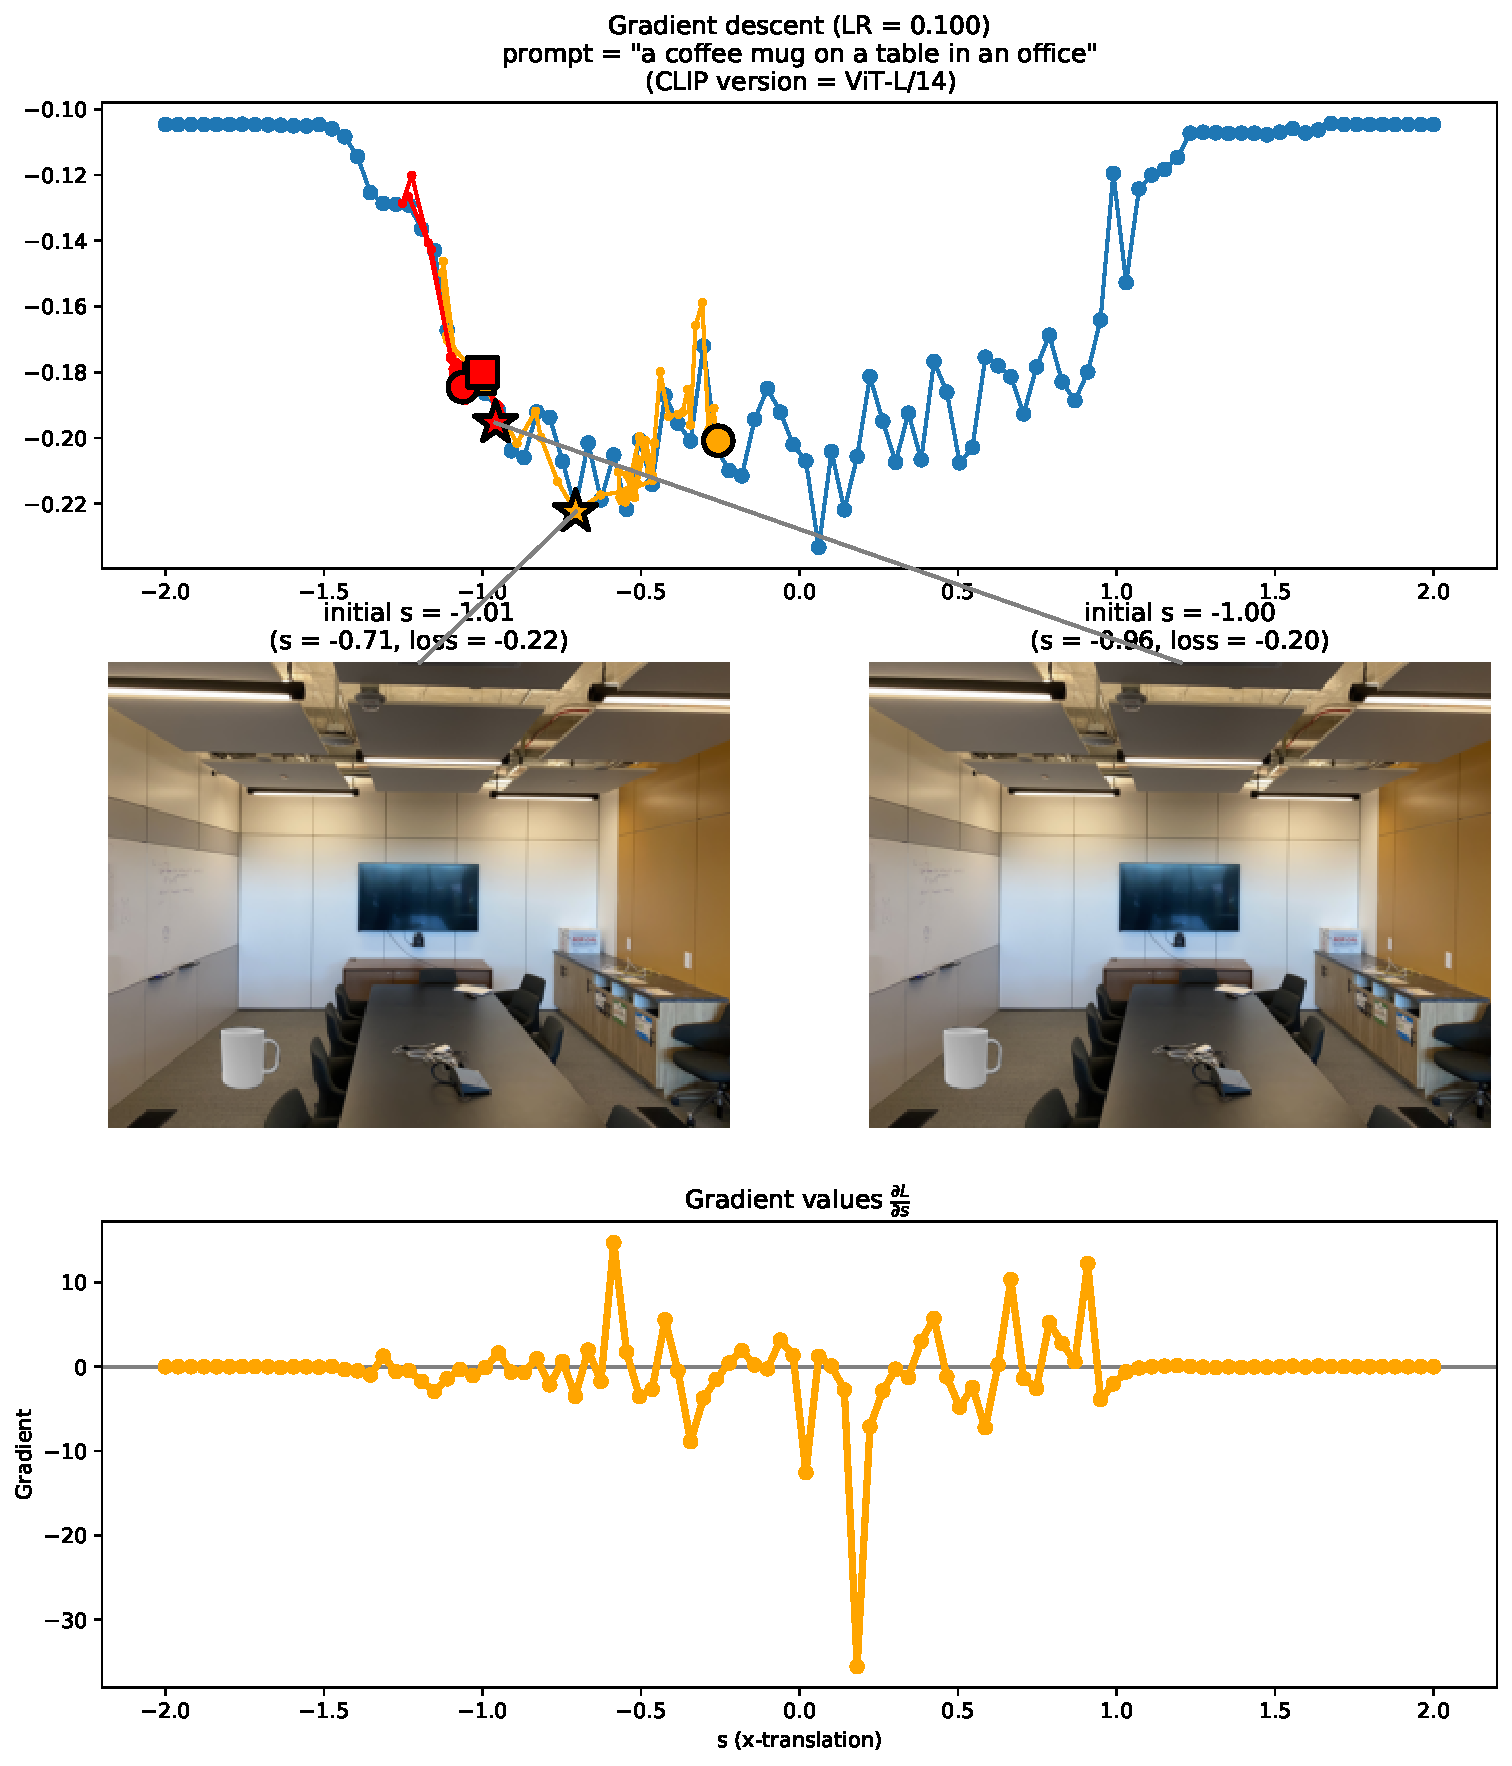
\includegraphics[width=1.0\textwidth]{figures/3_2-room-vanilla-gd.pdf}
    \caption{The top row shows the CLIP loss landscape overlaid with the gradient descent path (the square is the starting point, the circle is the final point, the star is the minimum value encountered during training). The middle row shows the image corresponding to the minimum found during gradient descent. The bottom row shows the gradient values for the sample $s$-values.}
    \label{fig:3_2-room-vanilla-gd}
\end{figure}

Figure \ref{fig:3_2-room-vanilla-gd} shows that gradient descent fails to locate the minimum. It also shows how two very similar initial conditions (i.e. initial $s={-1.01, -1}$) can end up yielding very different paths. The bottom row shows that the gradients are very noisy in the range $[-1,1]$.

% noisy loss pondering (shattered gradients)
So why does the loss function (and gradients, by extension) become so noisy? Recall what was presented in section \ref{sec:shattered-gradients} - essentially, it has a lot to do with the depth of the network used. Also recall that the CLIP model version "ViT-L/14" has been used for the experiments up until this point. Although skip connections are present both in the vision transformer and ResNet architectures, it might still be beneficial to switch the CLIP model to the shallowest ResNet CLIP architecture. Thus, the model was switched to a RN50 version. The results of this modification are shown in figure \ref{fig:3_2-room-vanilla-gd-rn50}.

\begin{figure}[H]
    \centering
    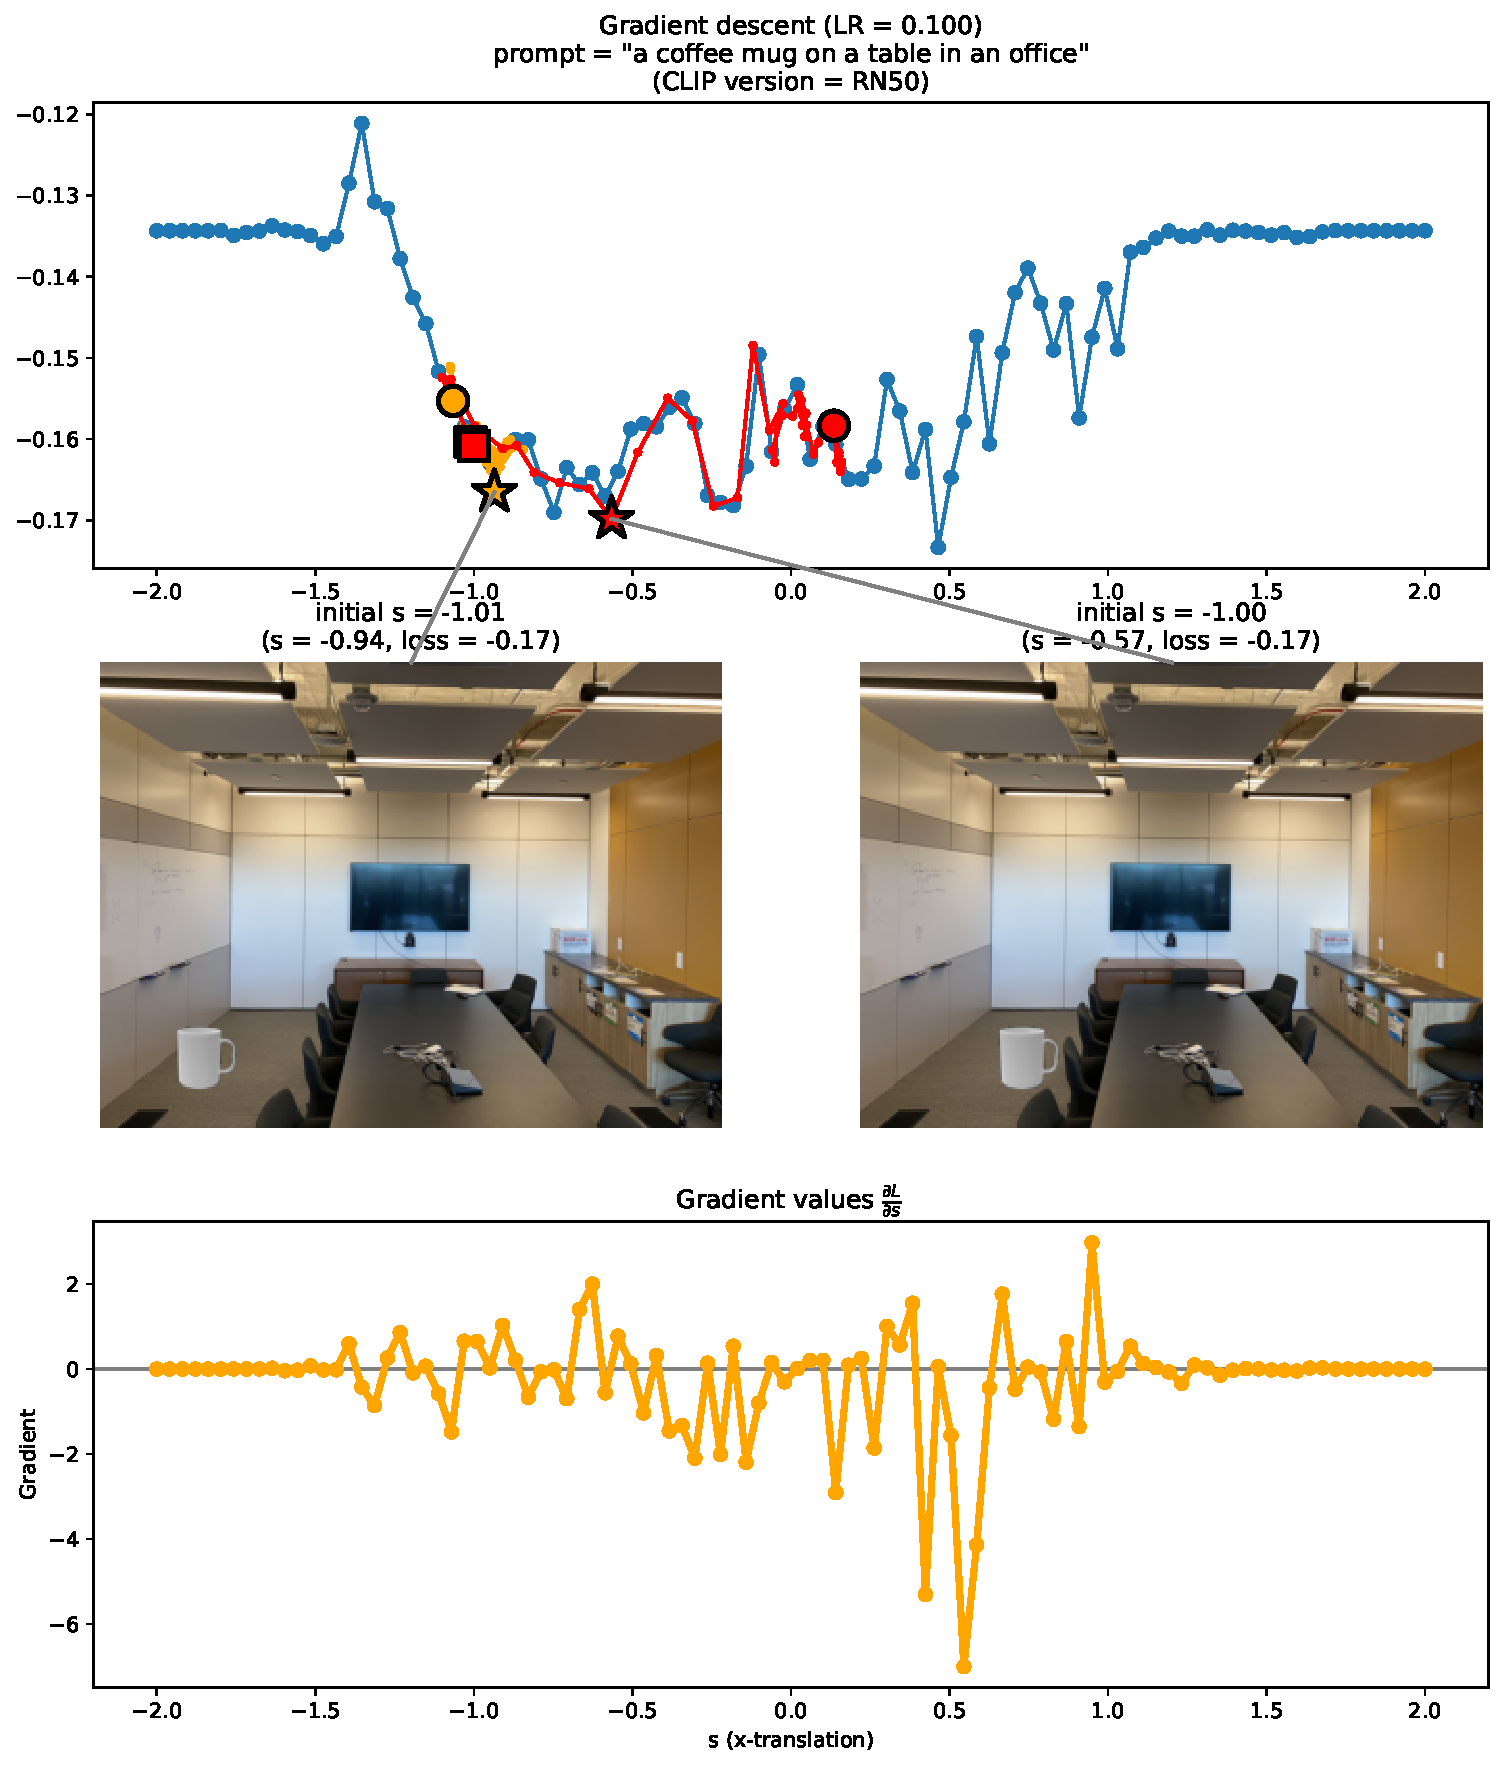
\includegraphics[width=1.0\textwidth]{figures/3_2-room-vanilla-gd-rn50.pdf}
    \caption{The top row shows the CLIP loss landscape overlaid with the gradient descent path (the square is the starting point, the circle is the final point, the star is the minimum value encountered during training). The middle row shows the image corresponding to the minimum found during gradient descent. The bottom row shows the gradient values for the sample $s$-values.}
    \label{fig:3_2-room-vanilla-gd-rn50}
\end{figure}

Figure \ref{fig:3_2-room-vanilla-gd-rn50} shows that the loss landscape is still rather noisy. The magnitude of the gradient extremes seems to have decreased. However, gradient descent still didn't manage to find the minimum. Alas, choosing a shallower CLIP model did not seem to improve things much.

% gradient descent round two!
There exists other techniques which could potentially improve the performance of gradient descent: \noindent
\begin{itemize}[noitemsep]
    \setlength\itemsep{0.5em}
    \item Gradient clipping/scaling
    \item Provide an ensemble of different text prompts
    \item Random image augmentations
    \item Using an ensemble of CLIP models
\end{itemize}
An experiment was performed where all modifications except the last one were implemented. The gradients were clipped at $\pm3$. An additional two text prompts were provided (replacing "coffee mug" with "cup of coffee" and "white mug"). 8 random image augmentations were applied at every render. The image augmentations consisted of different operations from \textit{kornia}: [RandomElasticTransform, ColorJitter, RandomHorizontalFlip, RandomGaussianBlur, RandomGrayscale]. Again, the same learning rate of 0.1 and iteration count of 300 was used. The results can be seen in figure \ref{fig:3_2-room-megaaugment-gd}.

\begin{figure}[H]
    \centering
    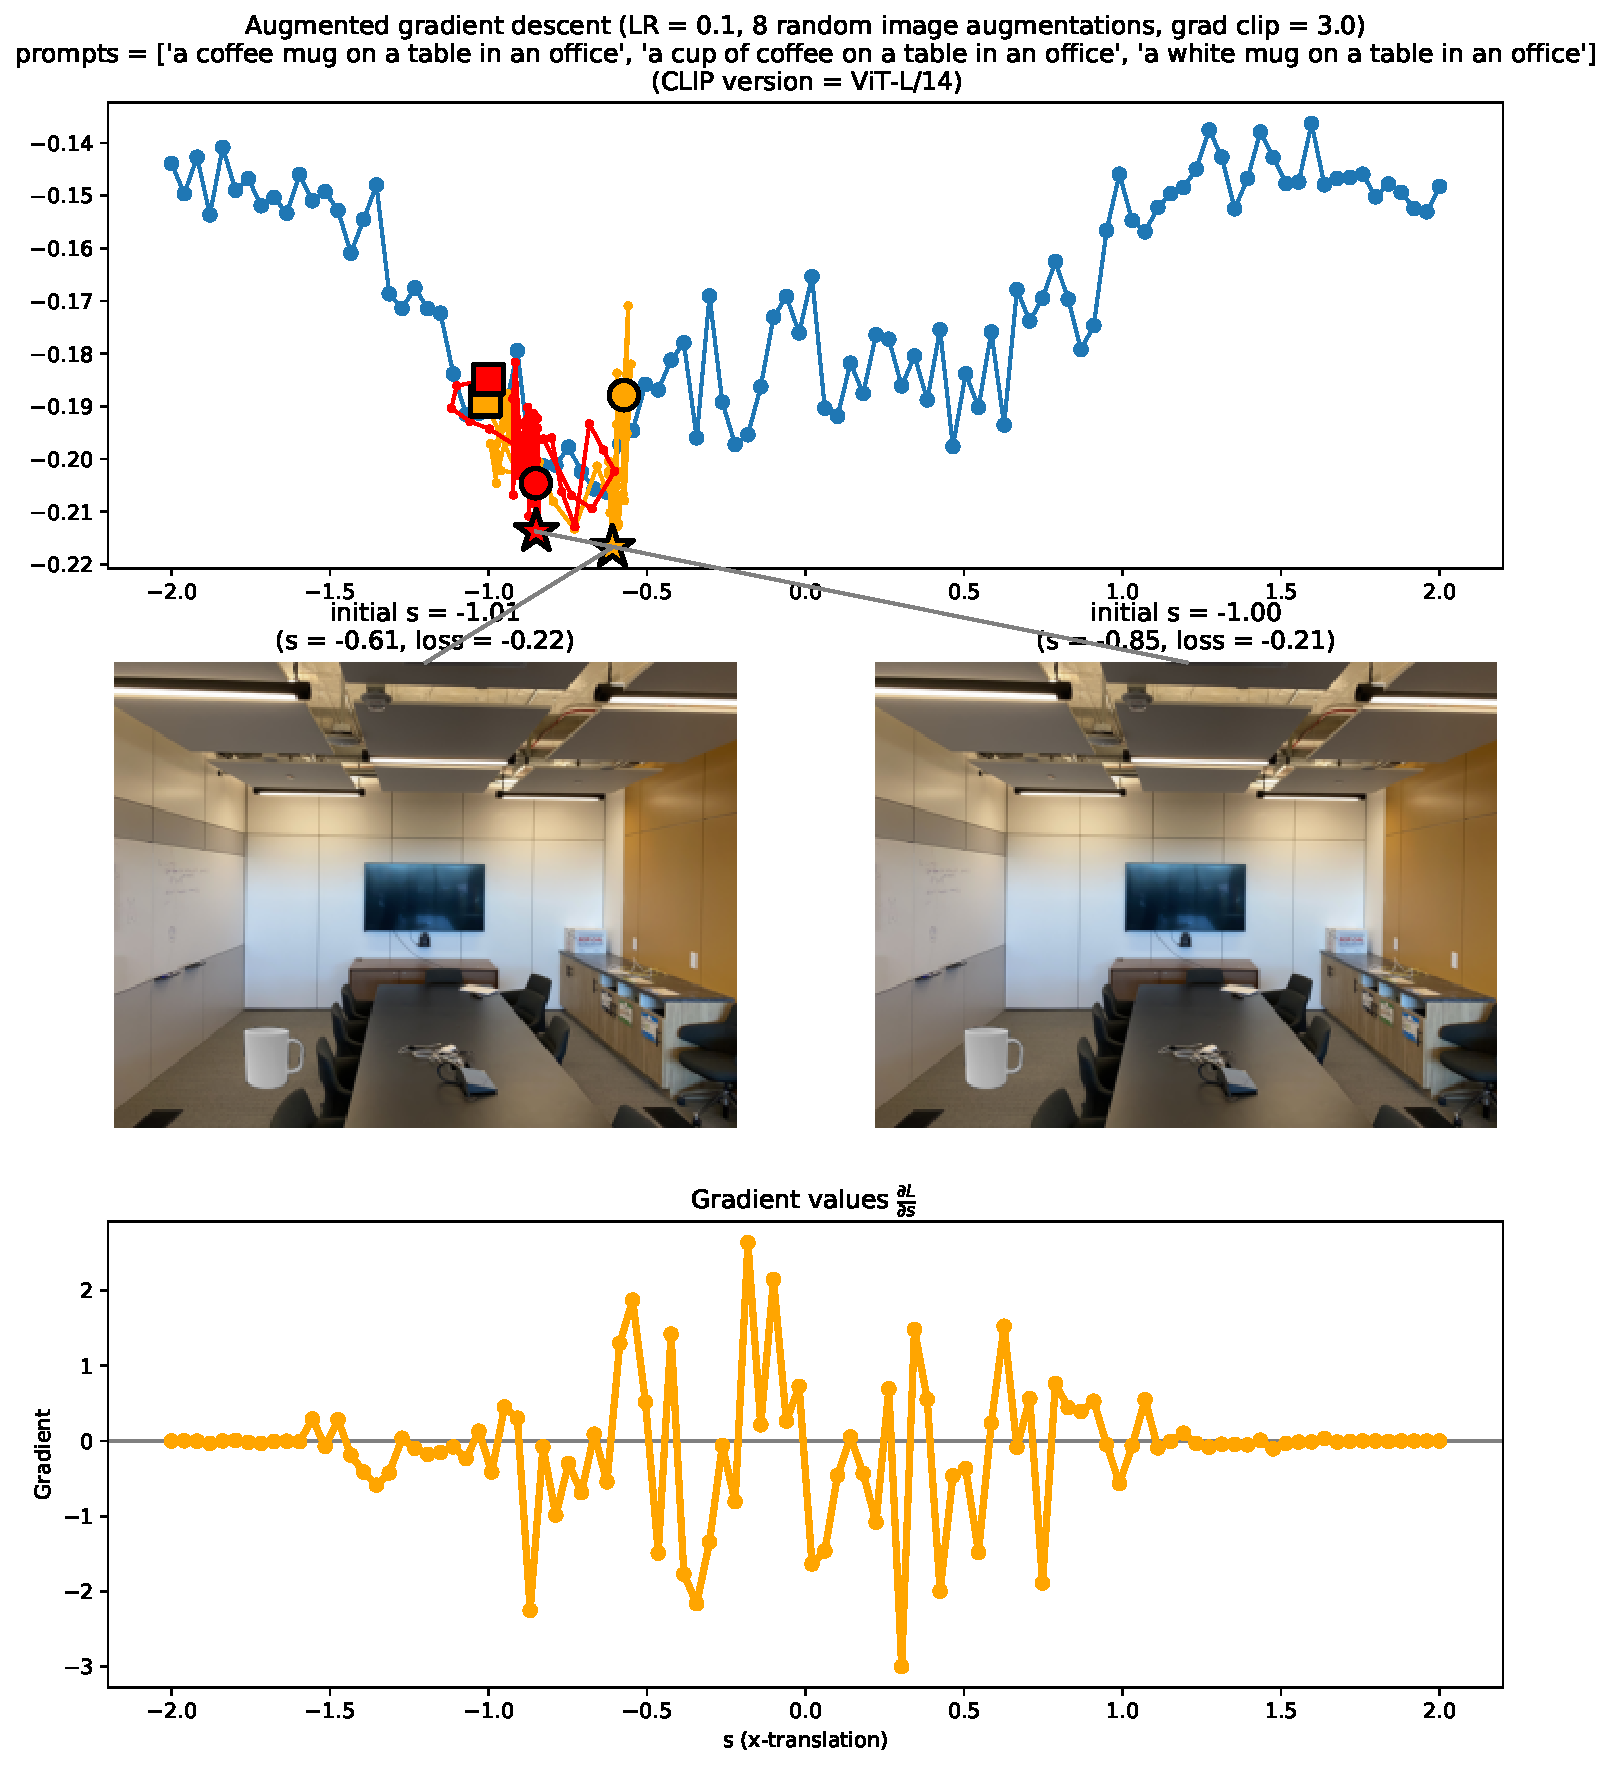
\includegraphics[width=1.0\textwidth]{figures/3_2-room-megaaugment-gd.pdf}
    \caption{Augmented gradient descent. The top row shows the CLIP loss landscape overlaid with the gradient descent path (the square is the starting point, the circle is the final point, the star is the minimum value encountered during training). The middle row shows the image corresponding to the minimum found during gradient descent. The bottom row shows the gradient values for the sample $s$-values.}
    \label{fig:3_2-room-megaaugment-gd}
\end{figure}

Figure \ref{fig:3_2-room-megaaugment-gd} shows that the loss landscape is not dramatically improved. In fact, the minimum seems to have moved away from around $s=0.0$ - it now appears to be between $-1.0$ and $-0.5$. However, the gradient descent final solutions do seem to end up slightly closer this time.


% bg blur augment
Taking a step back, one might notice that when the example was changed from the backgroundless mug scaling renderer to the office mug translation renderer, the loss landscape became even noisier. Perhaps the background is contributing a lot to the noise? An effective augmentation might be to blur the background using something like a Gaussian blur at multiple $\sigma$-values. Examples of this augmentation can be seen in figure \ref{fig:3_2-blur-examples}.
\begin{figure}[H]
    \centering
    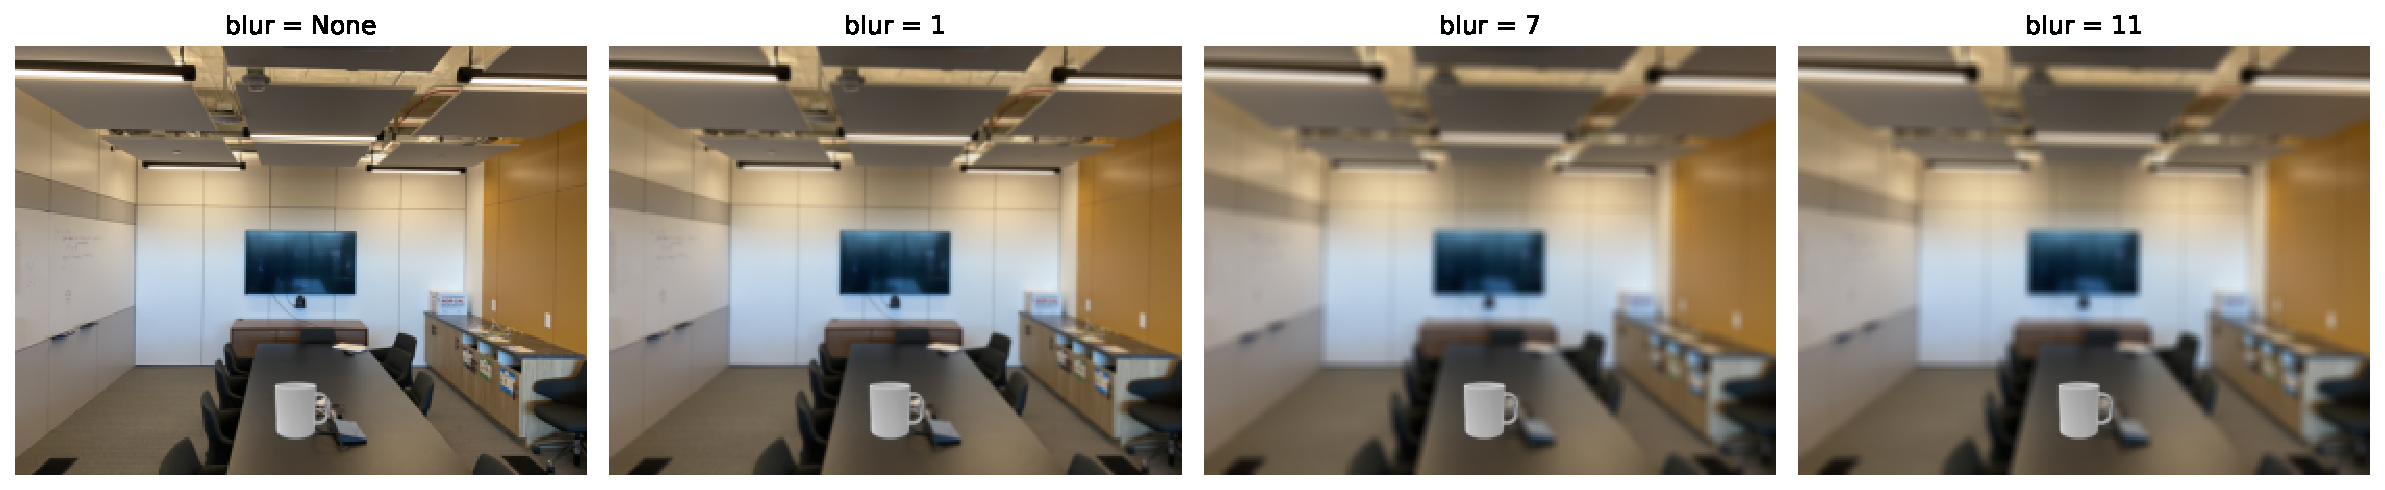
\includegraphics[width=1.0\textwidth]{figures/3_2-blur-examples.pdf}
    \caption{Examples of the described background blur augmentation}
    \label{fig:3_2-blur-examples}
\end{figure}


The augmentation procedure produced 4 images at every render evaluation using $\sigma=[None, 3, 7, 11]$. The same gradient descent training loop is used, except the learning rate is increased to $0.2$. This produced the results seen in figure \ref{fig:3_2-room-augment-gd}.
Figure \ref{fig:3_2-room-augment-gd} shows a less noisy loss landscape. The two different initial conditions also seem to lead to more similar paths than before (i.e. the landscape is less chaotic now). Alas, the augmentation had an arguably positive impact.

\begin{figure}[H]
    \centering
    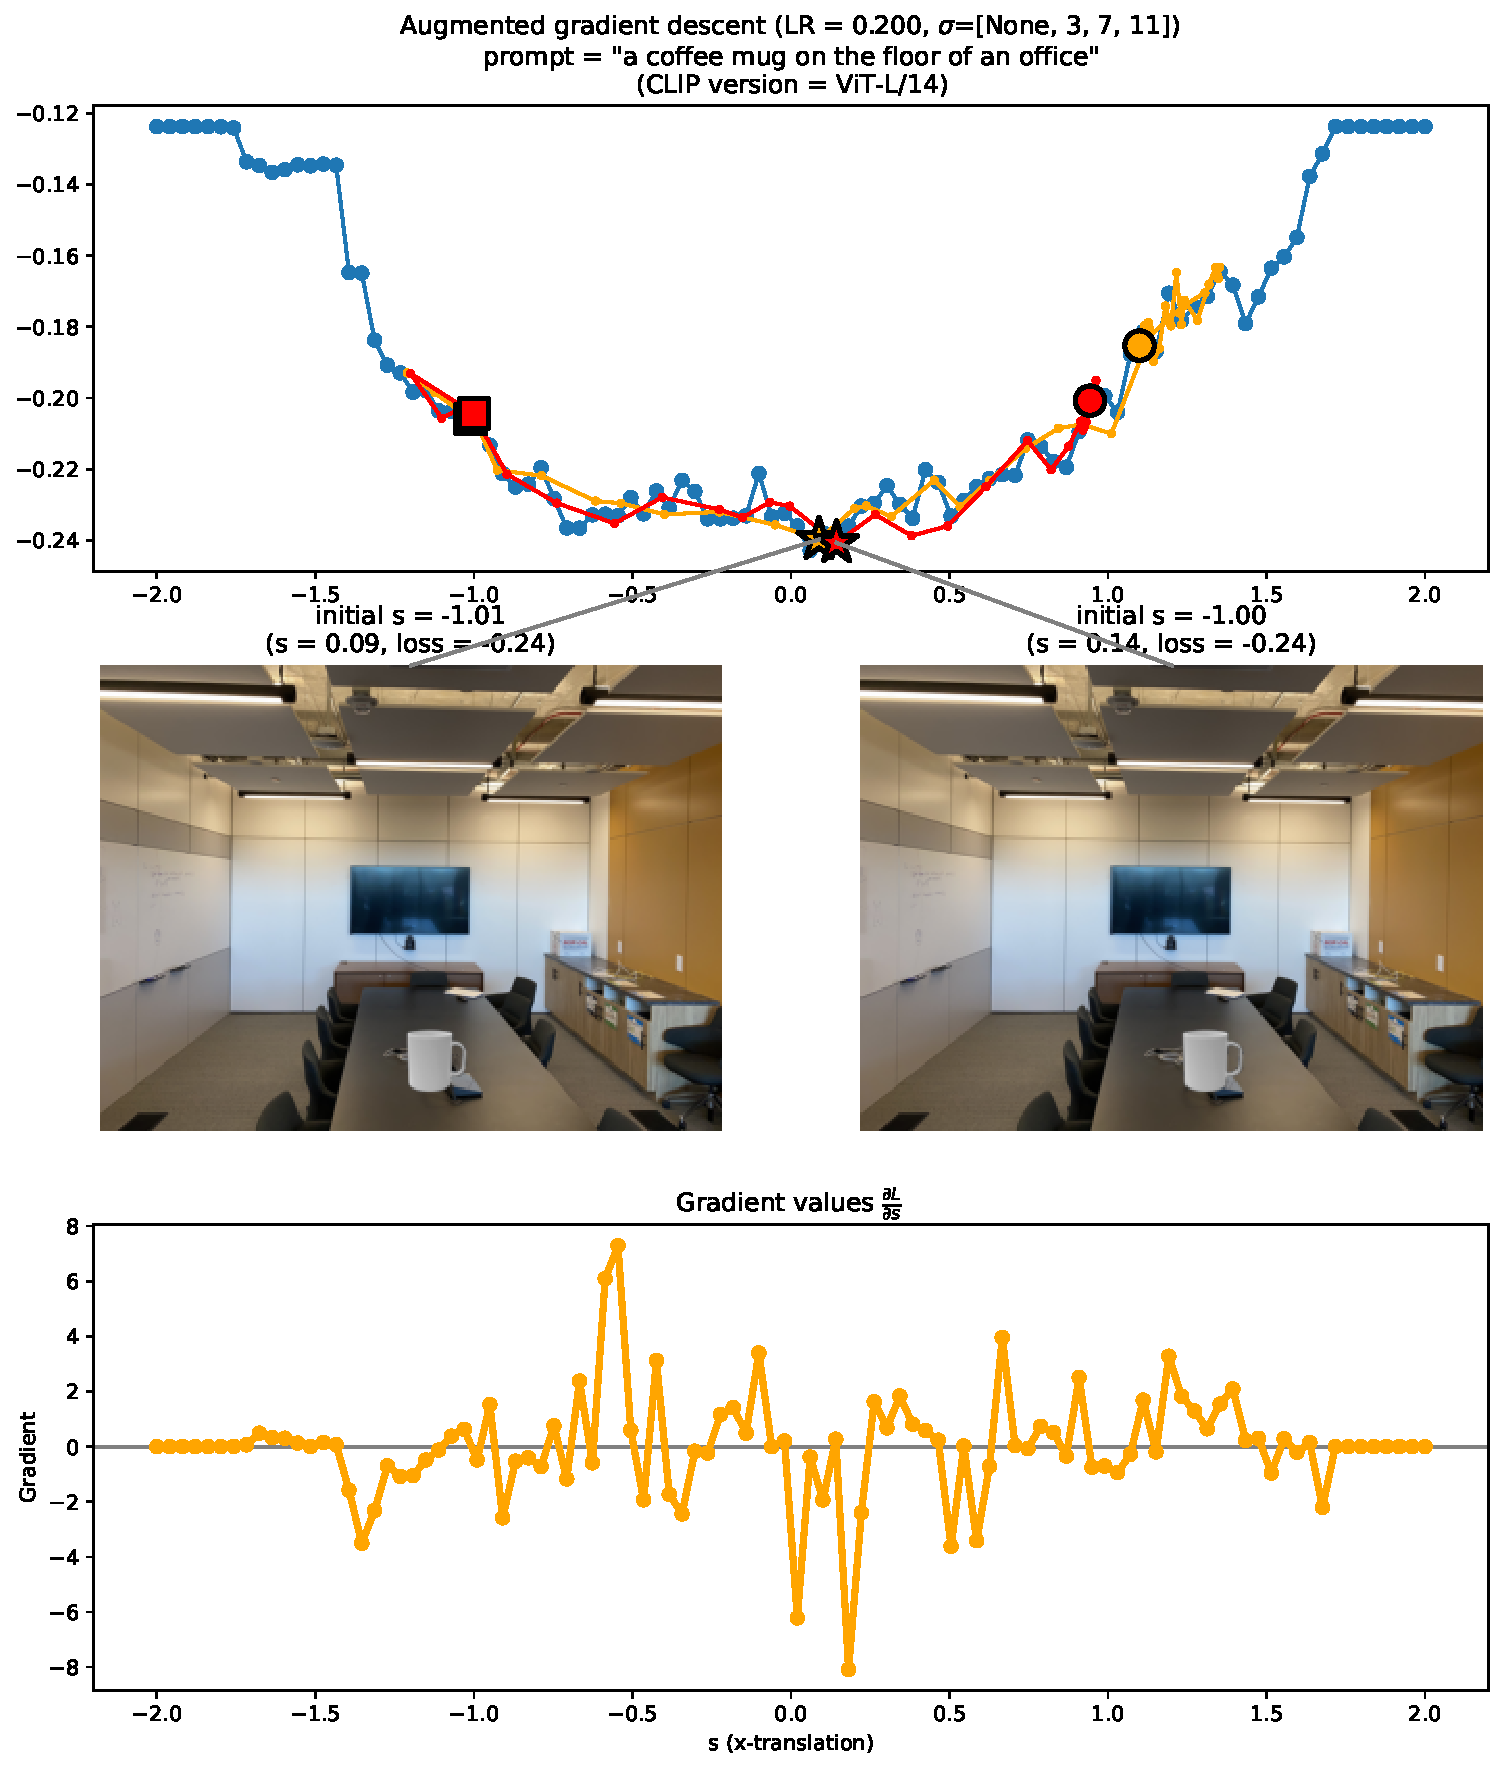
\includegraphics[width=1.0\textwidth]{figures/3_2-room-augment-gd.pdf}
    \caption{Background-blur augmentation gradient descent. The top row shows the CLIP loss landscape overlaid with the gradient descent path (the square is the starting point, the circle is the final point, the star is the minimum value encountered during training). The middle row shows the image corresponding to the minimum found during gradient descent. The bottom row shows the gradient values for the sample $s$-values.}
    \label{fig:3_2-room-augment-gd}
\end{figure}

% gradient analysis
A comparison of the gradients was made in order to validate if the gradients differ in terms of noise. The gradients from the bottom rows of figures \ref{fig:3_2-room-vanilla-gd}, \ref{fig:3_2-room-vanilla-gd-rn50}, \ref{fig:3_2-room-augment-gd} were gathered at a higher resolution this time ($N=100 \rightarrow N=300$ values of $s$). The collected gradients (along with their empirical mean and standard deviation) can be seen in the first row of \ref{fig:3_2-gradients-acf}. As explained in section\ref{sec:shattered-gradients}, the autocorrelation function (ACF) for the gradients can be plotted in order to visually validate noisiness. This can be seen in the bottom row of \ref{fig:3_2-gradients-acf}.
\begin{figure}[H]
    \centering
    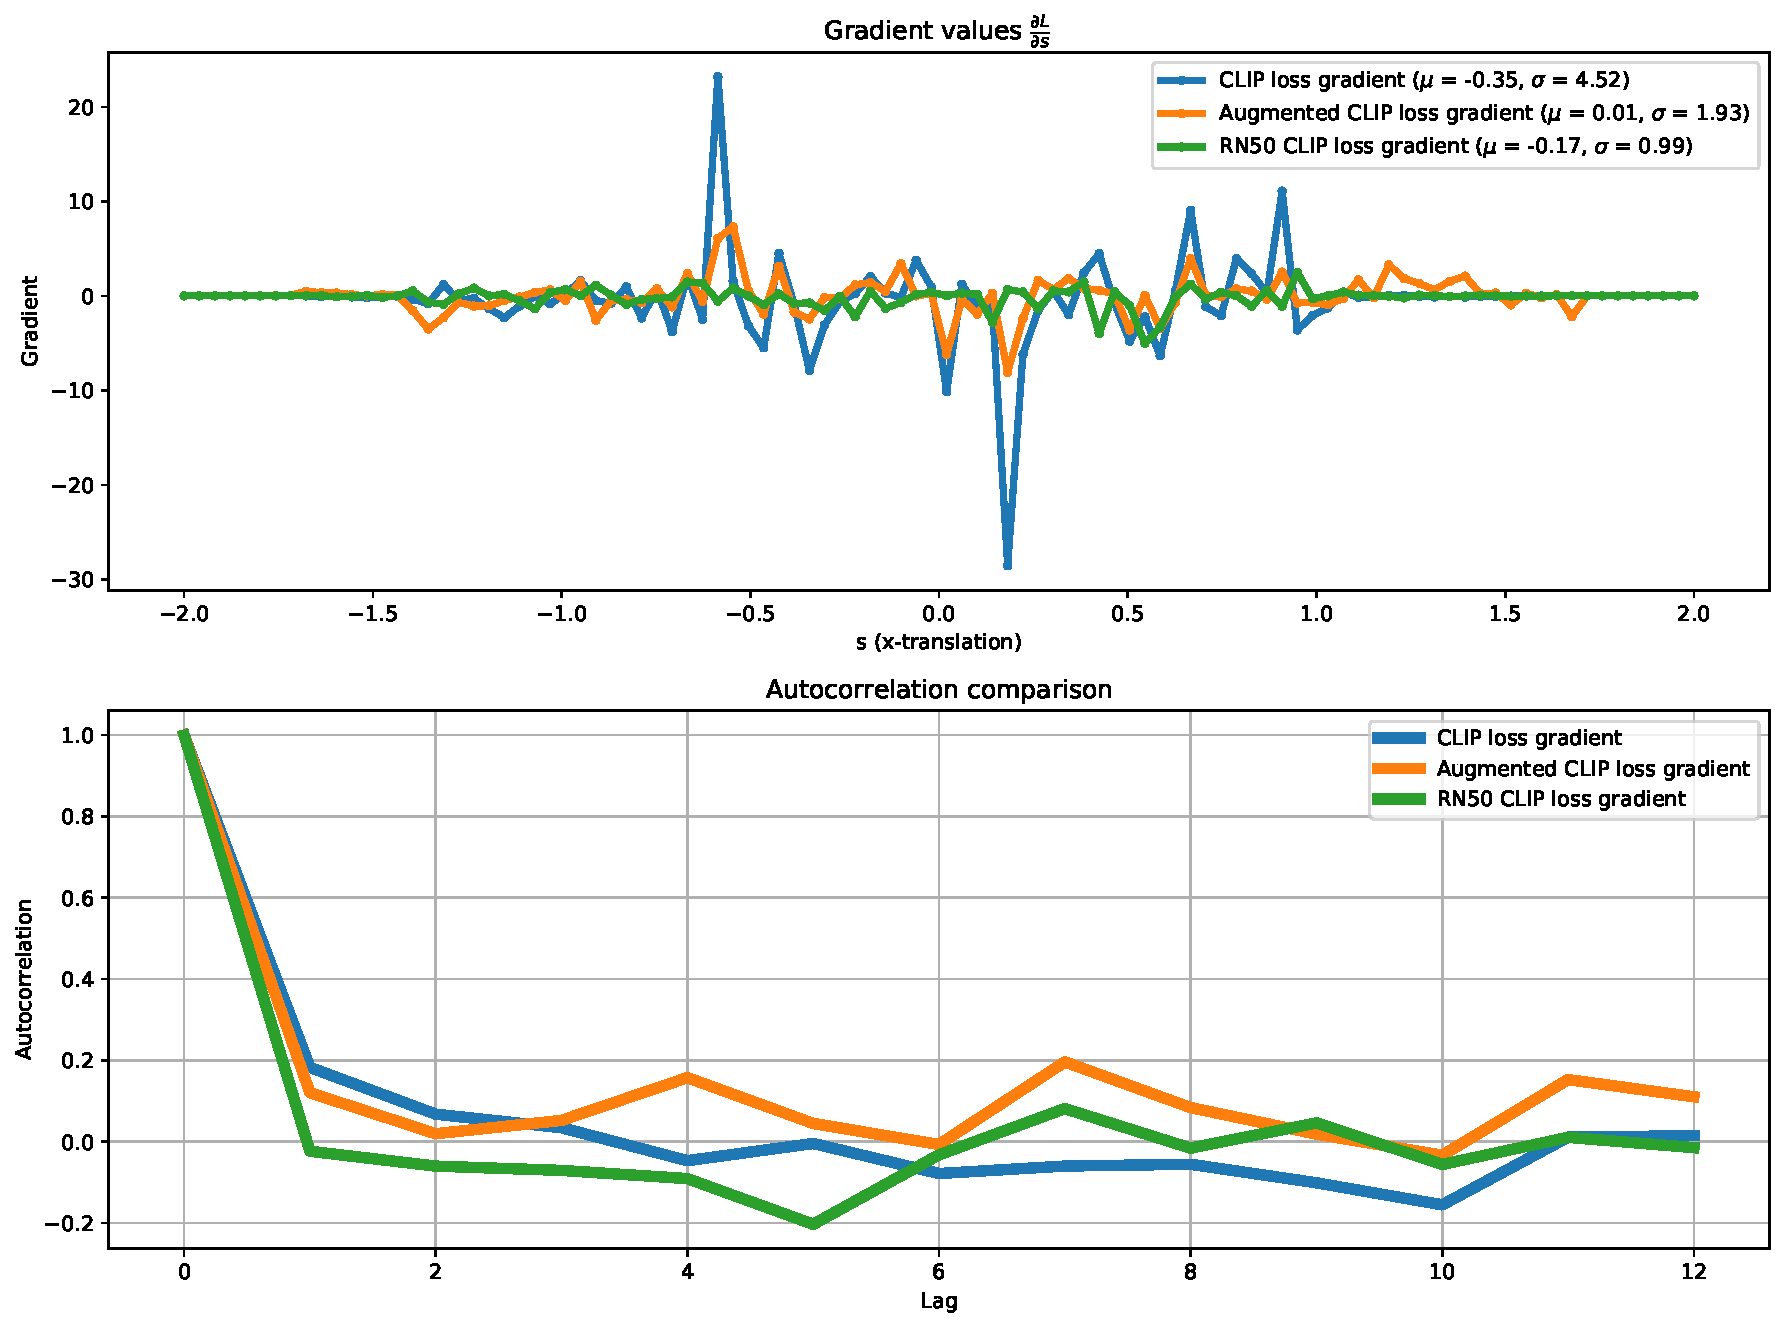
\includegraphics[width=1.0\textwidth]{figures/3_2-gradients-acf.pdf}
    \caption{Top row shows the gradients plotted with each other, with the calculated statistics in the legend. Bottom row shows the autocorrelation function for the various gradients.}
    \label{fig:3_2-gradients-acf}
\end{figure}

The top row of \ref{fig:3_2-gradients-acf} shows that there are quite a few drastic spikes of significant magnitudes in the unmodified gradients. The RN50 and augmented gradients don't exhibit the same spikes. The statistics in the legend also state that the mean values for the gradients are pretty similar (spans from $0.01$ to $-0.35$), but the standard deviation varies significantly between the different gradients (spans from $0.99$ to $4.52$). Alas, it seems that the RN50 gradients and the augmented gradients are pretty close to each other when compared to the unmodified gradients.

The bottom row of \ref{fig:3_2-gradients-acf} shows a comparison of the autocorrelation functions. For context, the ACF for a white noise process will quickly tend towards 0. With that in mind, it seems that every gradient is less random than a white noise process. While there isn't an overwhelming difference between the gradients, it does arguably look like the augmented gradients differ from 0 the most.

% multiparam
A multiparameter renderer was constructed. In addition to x-translation, the renderer also had 3 additional parameters for controlling scale, rotation and y-translation - thus, 4 parameters in total. An analogous gradient descent training loop was set up. The blur augmentation is applied, and the learning rate is decreased to 0.001. The loop is run for 300 iterations, and the results can be seen in figure \ref{fig:3_2-multiparam-loss-graph}.

\begin{figure}[H]
    \centering
    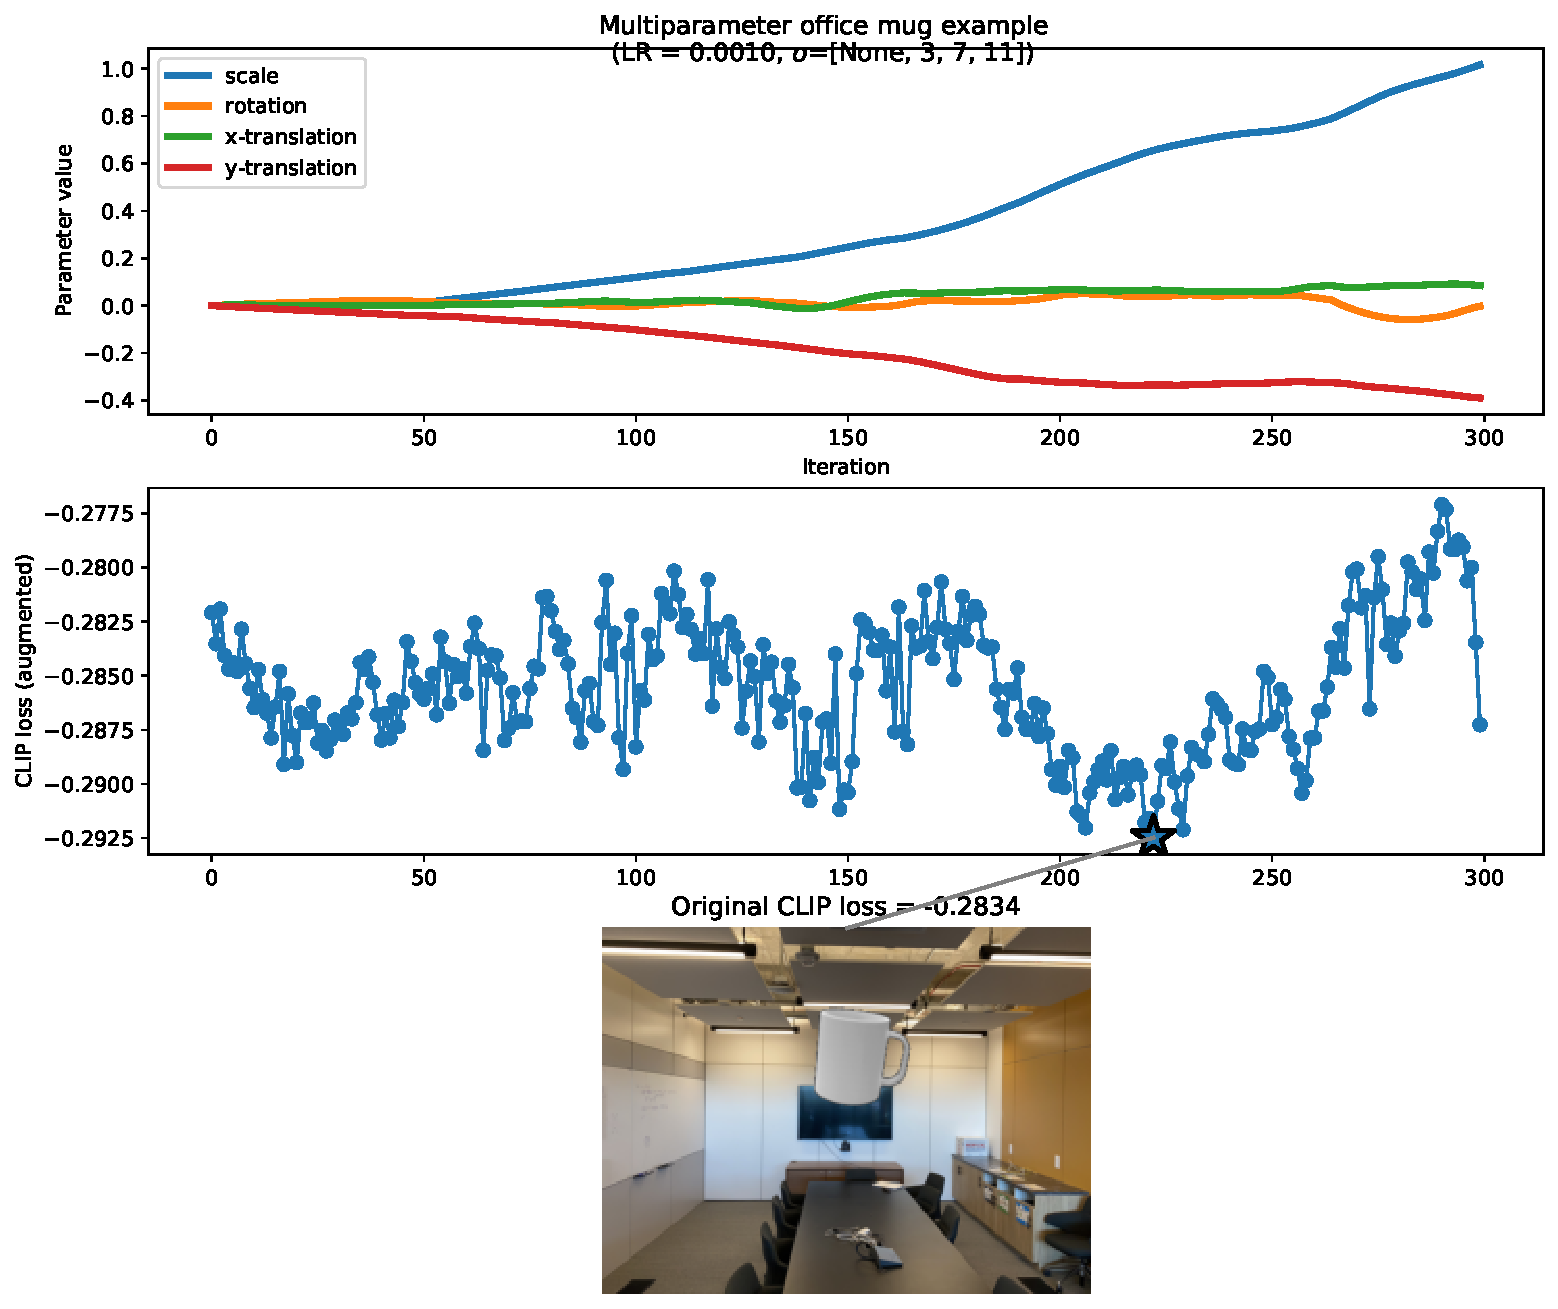
\includegraphics[width=1.0\textwidth]{figures/3_2-multiparam-loss-graph.pdf}
    \caption{Top row shows how the renderer parameters evolve over time. The middle row shows how the augmented CLIP loss evolves over time. The bottom row shows the image for the minimum encountered augmented CLIP loss, with the original CLIP loss written on top.}
    \label{fig:3_2-multiparam-loss-graph}
\end{figure}


% compare to brute force
A brute force search grid was constructed for the multiparameter renderer with a granularity of 20 for each parameter. Thus, the entire search space consists of $20^4=160.000$ parameter combinations. The brute force search took just under 2 hours to finish. The top three resulting images from the brute force search can be seen in \ref{fig:3_2-brute-force}

\begin{figure}
    \centering
    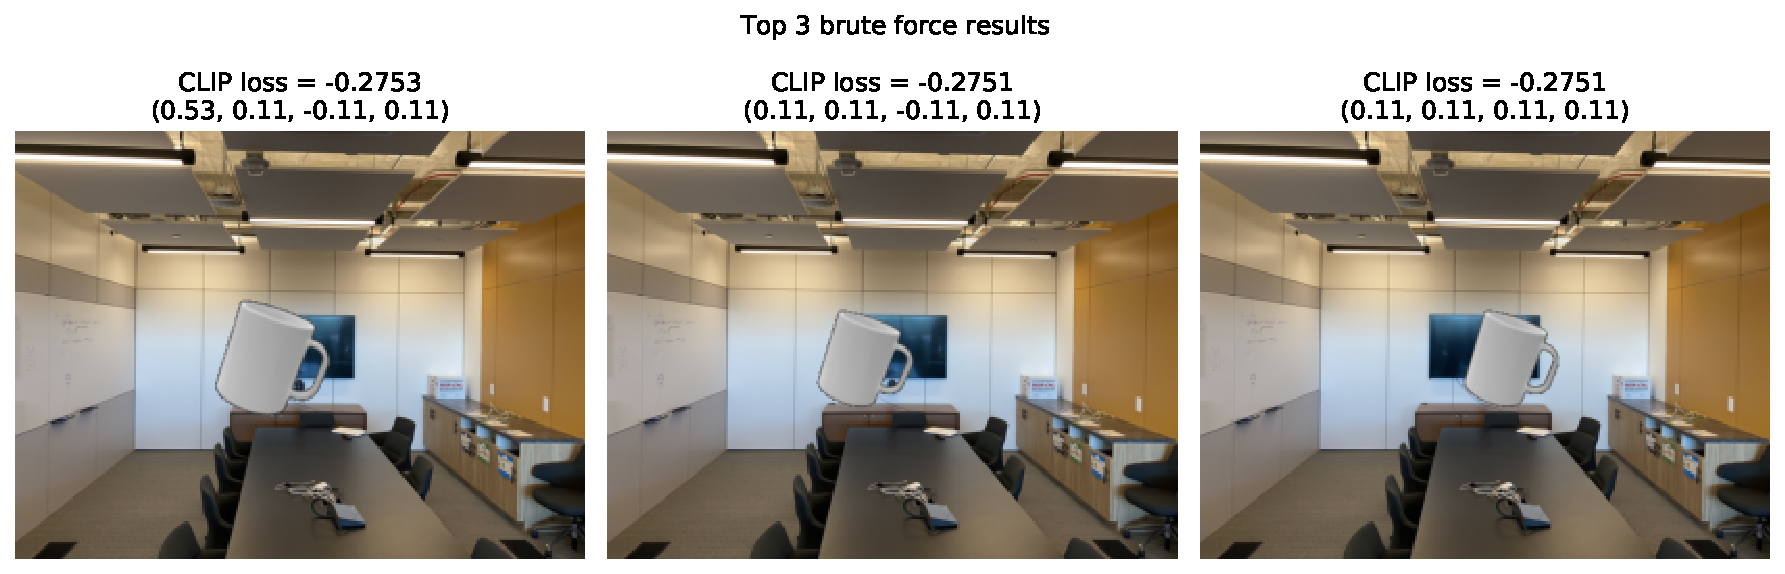
\includegraphics[width=1.0\textwidth]{figures/3_2-brute-force.pdf}
    \caption{Top three results from the brute force search. The corresponding CLIP losses have been written on top of each image.}
    \label{fig:3_2-brute-force}
\end{figure}

From figure \ref{fig:3_2-brute-force}, it appears that best results from the brute force search yield losses of $-0.2753, -0.2751, -0.2751$. These losses are all higher than the minimum loss found during gradient descent ($0.2834$). Alas, the brute force fails to find a more optimal solution than gradient descent for the multiparameter case.


To summarize the findings of this subchapter:
% subchapter recap
\begin{itemize}[noitemsep]
    \item CLIP loss is very noisy and non-convex - even for simple images such as the mug with no background.

    \item CLIP loss is very sensitive to the rendering parameters $s$ - i.e. very minuscule changes in $s$ can result in significant changes in CLIP loss.

    \item Gradient descent is very sensitive to initial conditions (e.g. initial $s$, learning rate, etc.)
    
    \item The most effective form of augmentation appeared to be the background blur augmentation. By observing the autocorrelation functions (ACF), it appears to slightly improve gradient noise.

    \item Determining the true global minimum for the CLIP loss is very difficult even for a brute force search. For the example with just 4 transformation parameters, gradient descent seems to win over brute force, both in regard to time complexity and loss minimization.
\end{itemize}


\section{3D semantic experiments}
Now it's time to move on to using a 3D rendering mechanism. There are many solutions that could be used here - NeRFs are just one possibility in this regard. Due to time constraints, an alternative differentiable rendering mechanism was used. The library pytorch3d\footnote{\url{https://pytorch3d.org/}} provides a differentiable renderer which works using meshes and textures. For the experiments, I found meshes and textures for a small toy cow and a wooden table.

% single param intro
Initially, a single-parameter 3D renderer was set up such that the parameter controls the y-translation of the cow (i.e. moves the cow vertically). The parameter is "bounded" using a $\tanh$ function, such that the cow never leaves the rendered image, even as $s \rightarrow \pm \infty$. Similar to the 2D mug translation example, a "sanity check" to see how a couple of example text prompts relate to the rendered image in terms of CLIP loss. Again, for the $s$-values, 100 linearly spaced samples from $[-2,2]$ are taken. The results can be seen in figure \ref{fig:3_3-cow-translation-optimal-images}.
\begin{figure}[H]
    \centering
    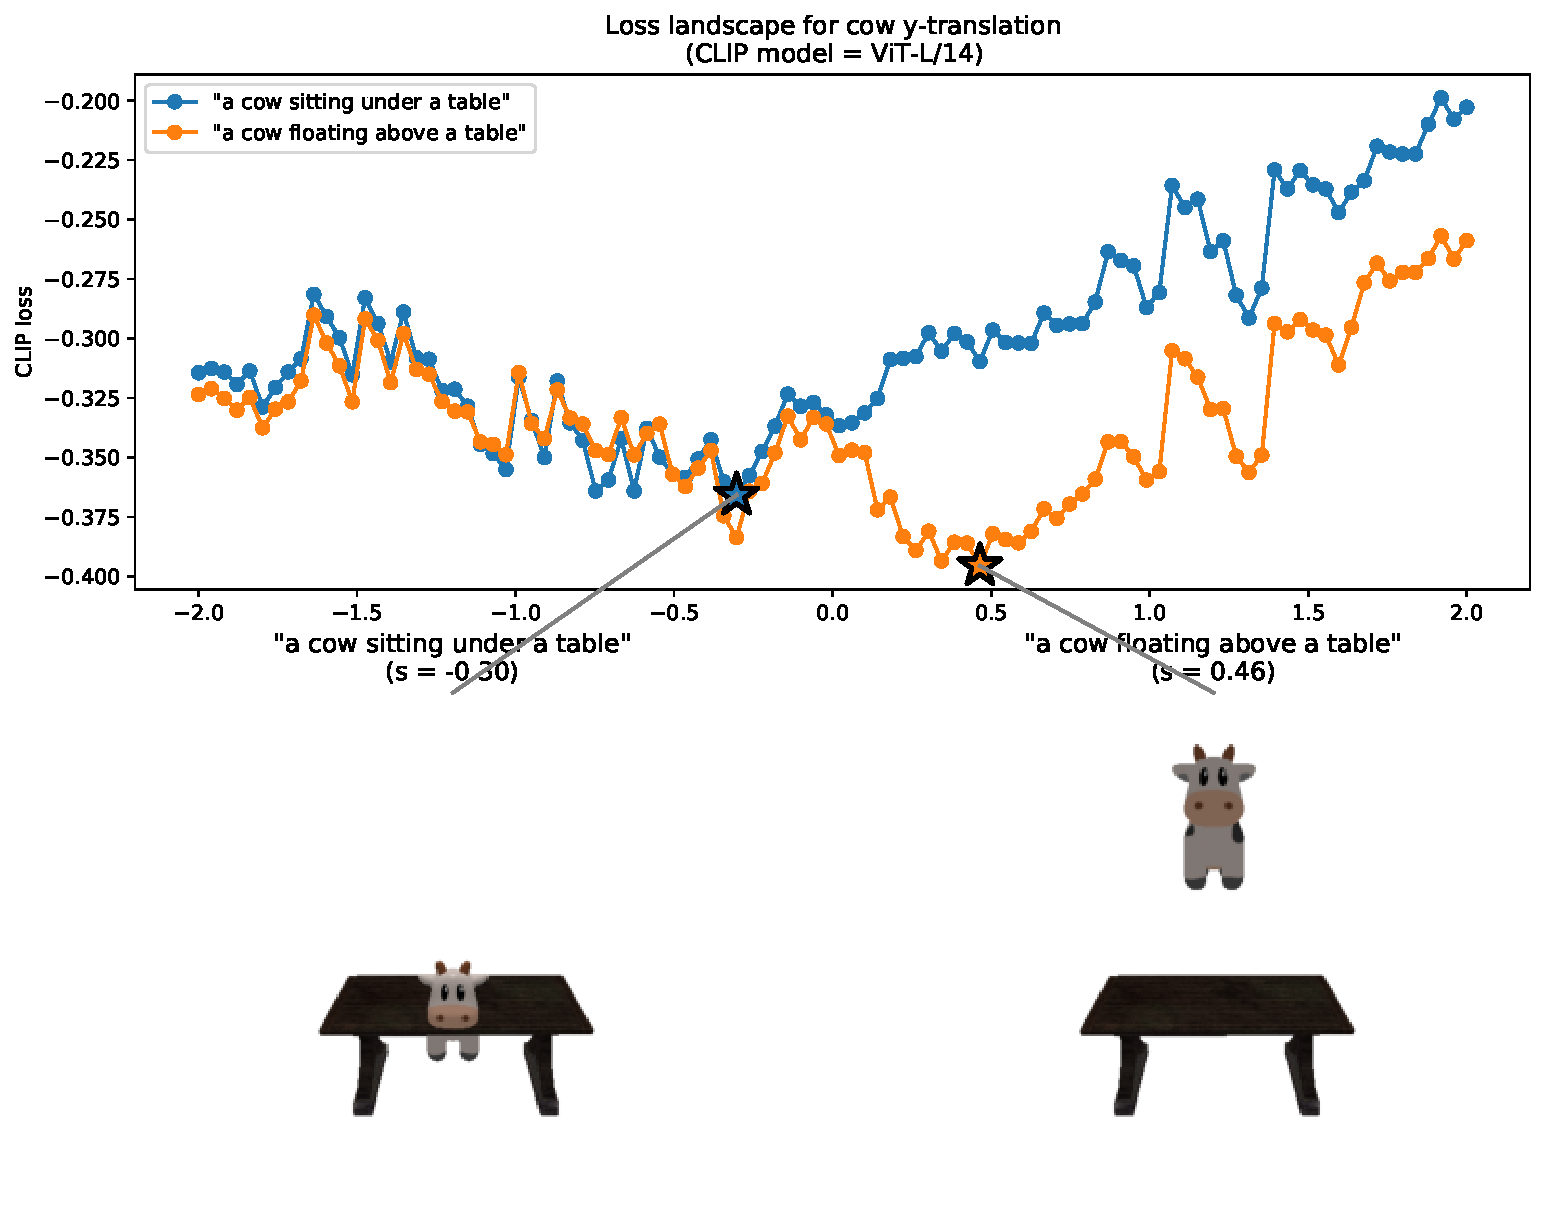
\includegraphics[width=1.0\textwidth]{figures/3_3-cow-translation-optimal-images.pdf}
    \caption{Top row shows the CLIP loss landscape for the different text prompts (star denotes the lowest encountered loss value for the corresponding text prompt). Bottom row shows how the rendered image looks for the corresponding parameter value.}
    \label{fig:3_3-cow-translation-optimal-images}
\end{figure}

Remarkably, the losses obtained in figure \ref{fig:3_3-cow-translation-optimal-images} are significantly lower than those for the mug examples from last subchapter (e.g. fig \ref{fig:3_2-room-translation-optimal-images}). The cow example reaches losses of almost $-0.40$, whereas the mug examples merely reached losses of about $-0.23$.

% single param - no augment
Now, the transformation is changed to z-translation (instead of y-translation). As the parameter value decreases, the z-translation will move the cow towards the camera, and, inversely, further away from the camera as the value increases.

An experiment is set up to see how well gradient descent performs for the single-parameter cow z-translation example. A training loop was constructed using Adam with initial LR = $0.05$ and a cosine annealing LR schedule. The loop is run for 300 iterations for each of the two starting points. The results can be seen in figure \ref{figs:3_3-cow-vanilla-gd}.

\begin{figure}[H]
    \centering
    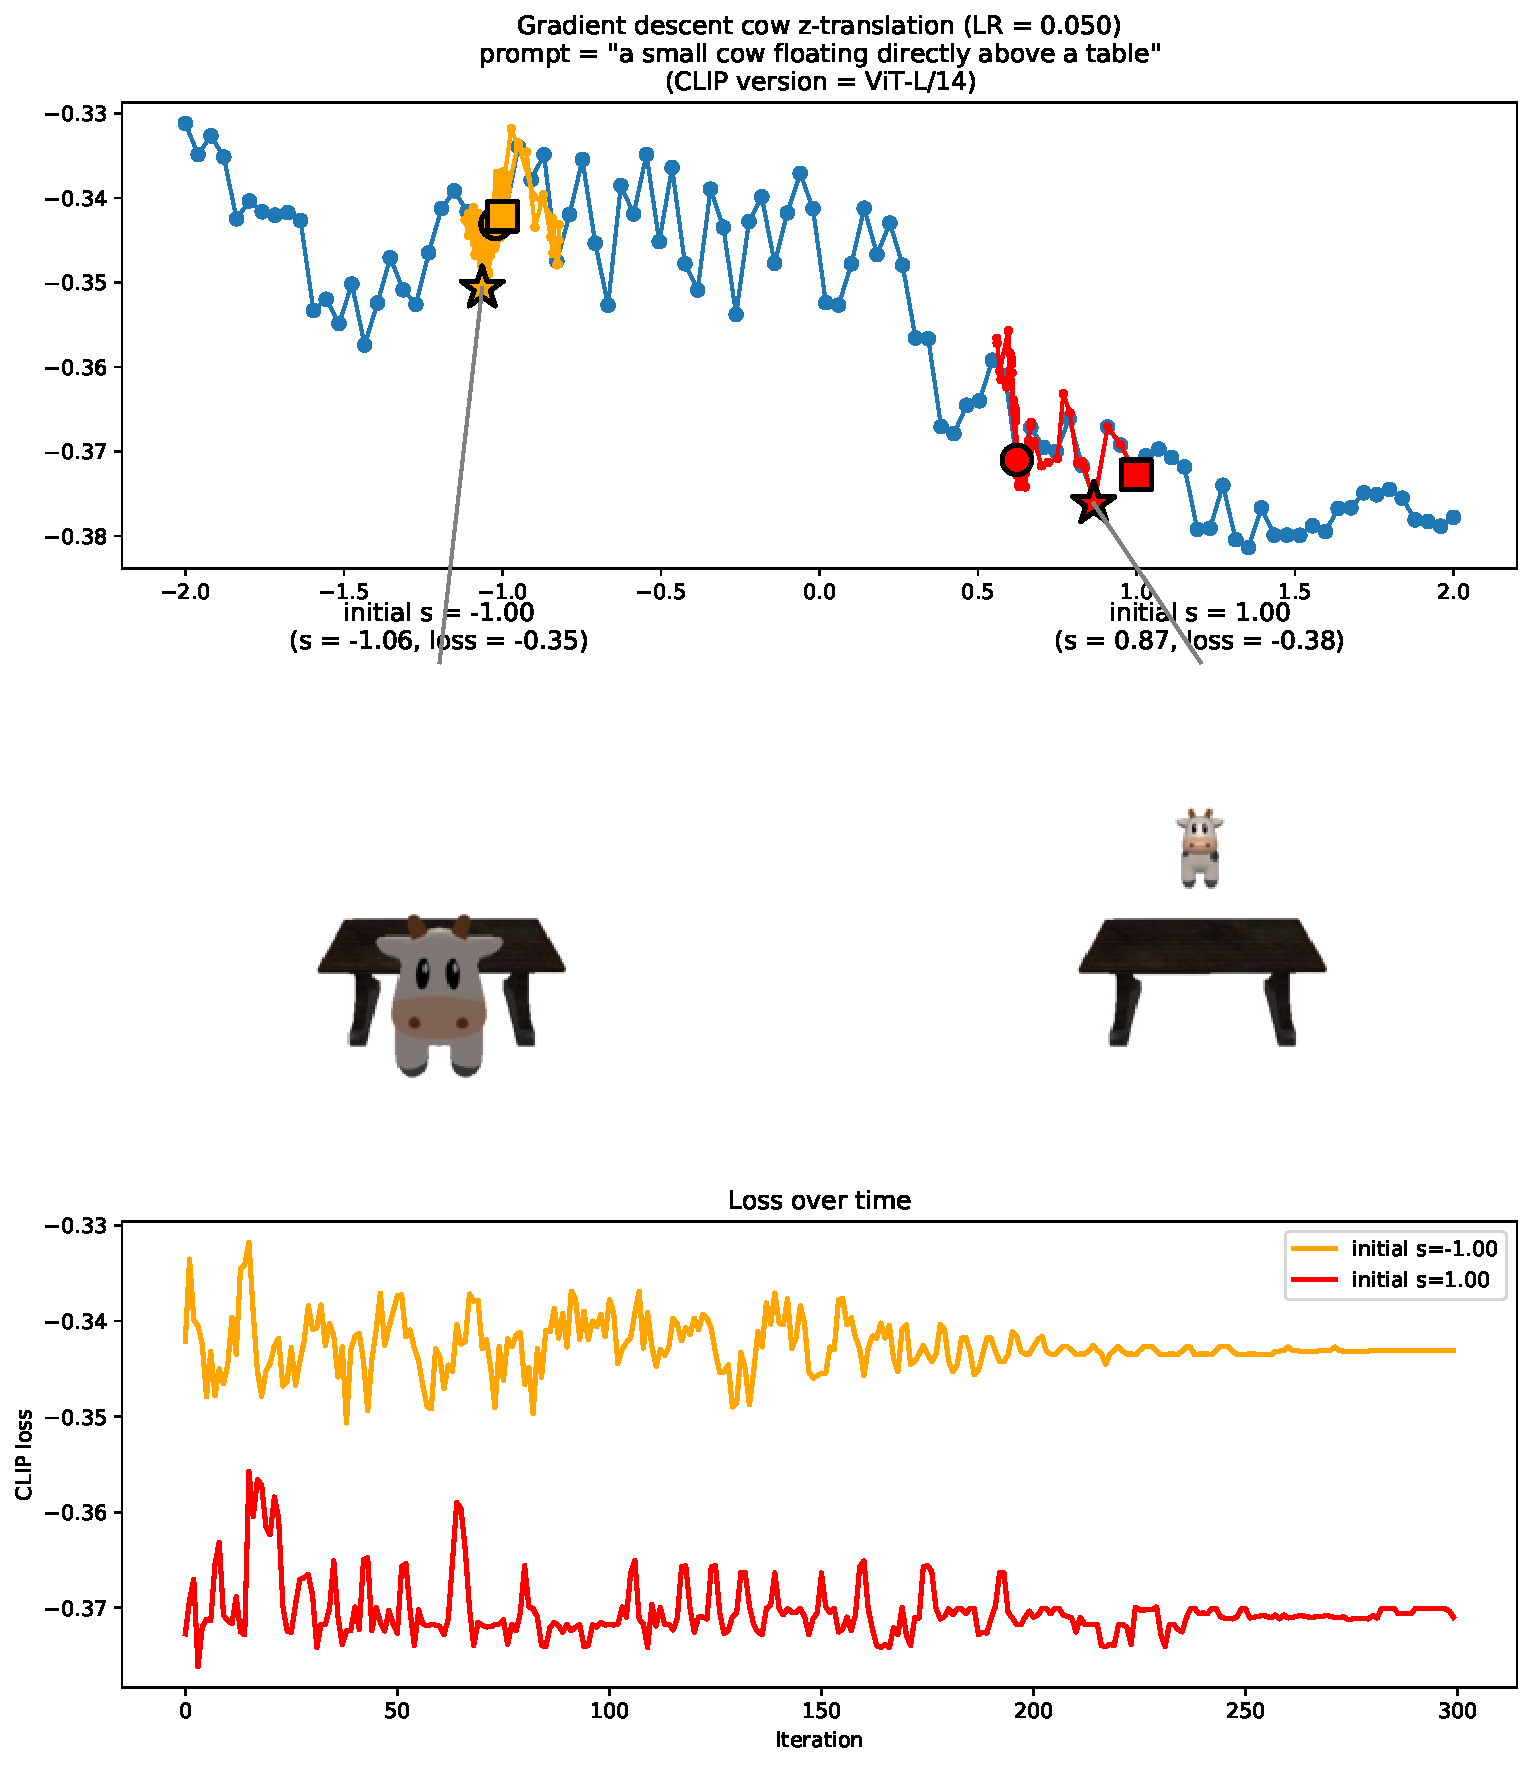
\includegraphics[width=1.0\textwidth]{figures/3_3-cow-vanilla-gd.pdf}
    \caption{Gradient descent for cow z-translation. Top row shows the loss landscape overlaid with the two gradient descent paths (square denotes starting point, circle denotes final iteration, star denotes lowest loss encountered). Middle row shows the produced images for the encountered minima. Bottom row shows the learning curve (i.e. loss over time) for the two runs.}
    \label{figs:3_3-cow-vanilla-gd}
\end{figure}

Figure \ref{figs:3_3-cow-vanilla-gd} shows that the gradient descent solutions don't end up in the global minimum. An important detail here is the fact that the loss landscape shows the most optimal $s$-value being around $s\approx1.5$. However, the value which actually places the cow directly above the table is $s=0$. This illustrates an underlying issue that has to do with the perspective from which the scene is observed. It appears that the scene needs to be rendered from multiple perspectives in order to obtain sufficient information about the cow's z-translation. The issue is illustrated in figure \ref{fig:3_3-cow-perspectives}.

\begin{figure}[H]
    \centering
    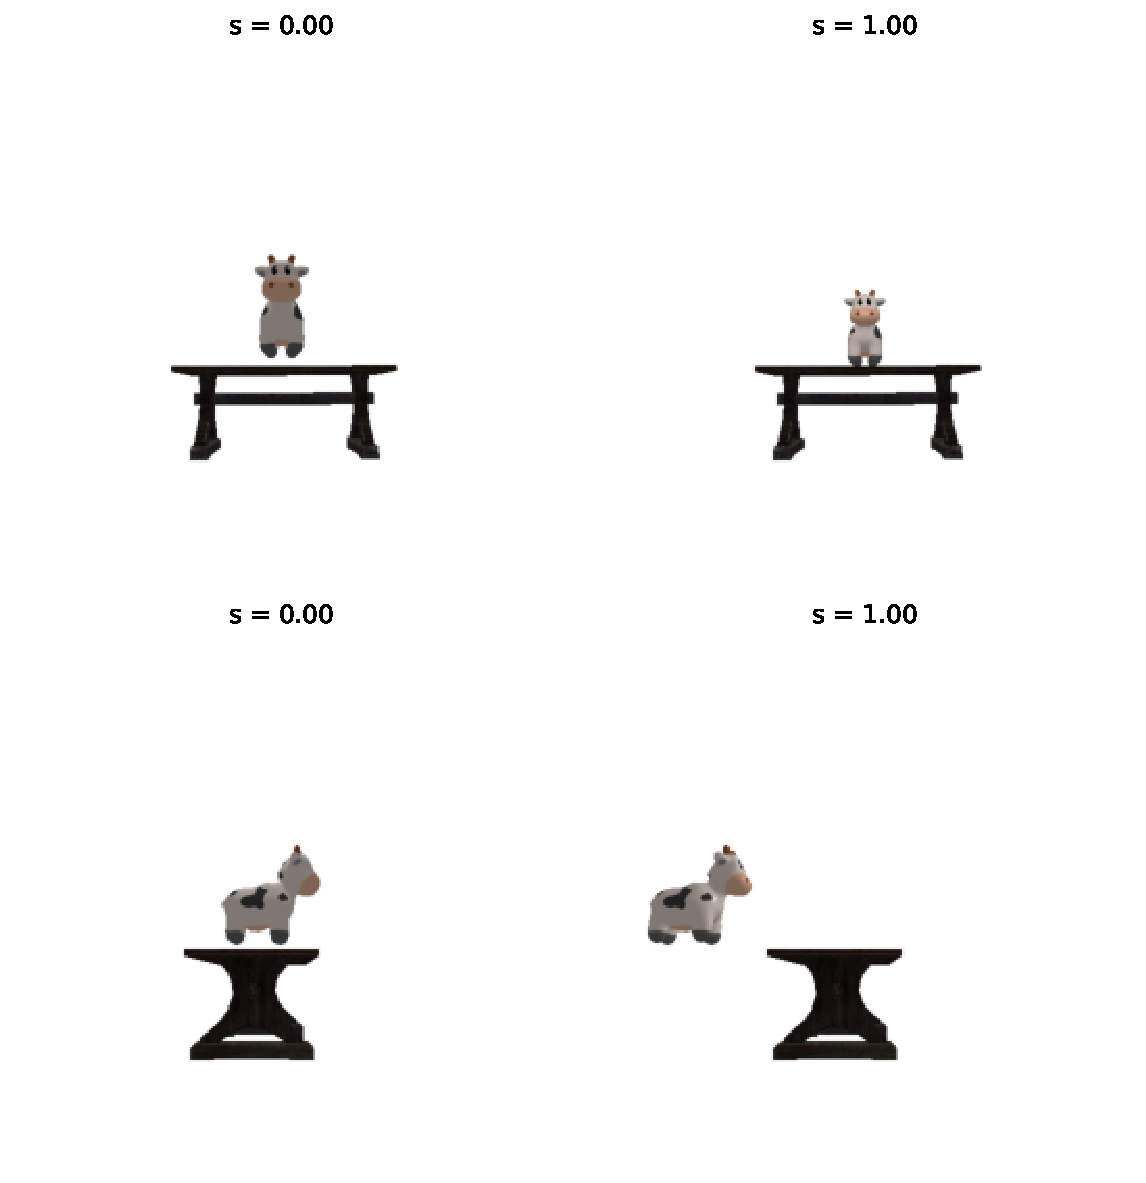
\includegraphics[width=0.75\textwidth]{figures/3_3-cow-perspectives.pdf}
    \caption{A demonstration of how perspectives can be confusing in 3D. The extent of the z-translation is not really clear from the perspective in the first row. The alternate perspective in the second makes it much easier to judge how far back the cow was moved.}
    \label{fig:3_3-cow-perspectives}
\end{figure}


% novel view augment intro
As a means of mitigating the issue of confusing perspectives in 3D, the next experiment attempts to explore the capabilities of novel view augmentation. The idea is to render multiple images of the scene seen from different perspectives, which can effectively be used as image augmentations. The exact process is illustrated in figure \ref{fig:3_3-novel-view-aug}.


\begin{figure}[H]
    \centering
    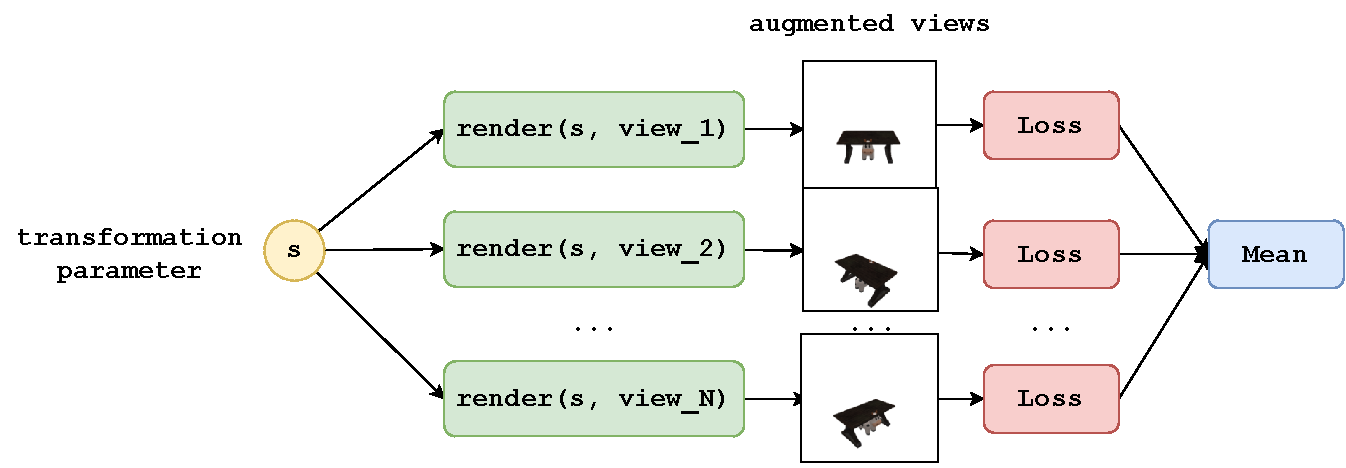
\includegraphics[width=1.0\textwidth]{figures/3_3-novel-view-aug.pdf}
    \caption{Overview of the novel view augmentation process}
    \label{fig:3_3-novel-view-aug}
\end{figure}


% single param - novel view augment
The training loop was replicated from the previous experiment (i.e. the experiment that produced fig \ref{figs:3_3-cow-vanilla-gd}), but it has the novel view augmentation this time. The alternate perspectives all had the same distance to the origin and the same elevation angle. The azimuth angle, however, was modulated by adding to it the degrees $[45, 90, 135, 180, 225, 270, 315]$ - this yielded a total of 8 rendered images per iteration. The results from running gradient descent are shown in figure \ref{fig:3_3-cow-aug-gd}.

\begin{figure}[H]
    \centering
    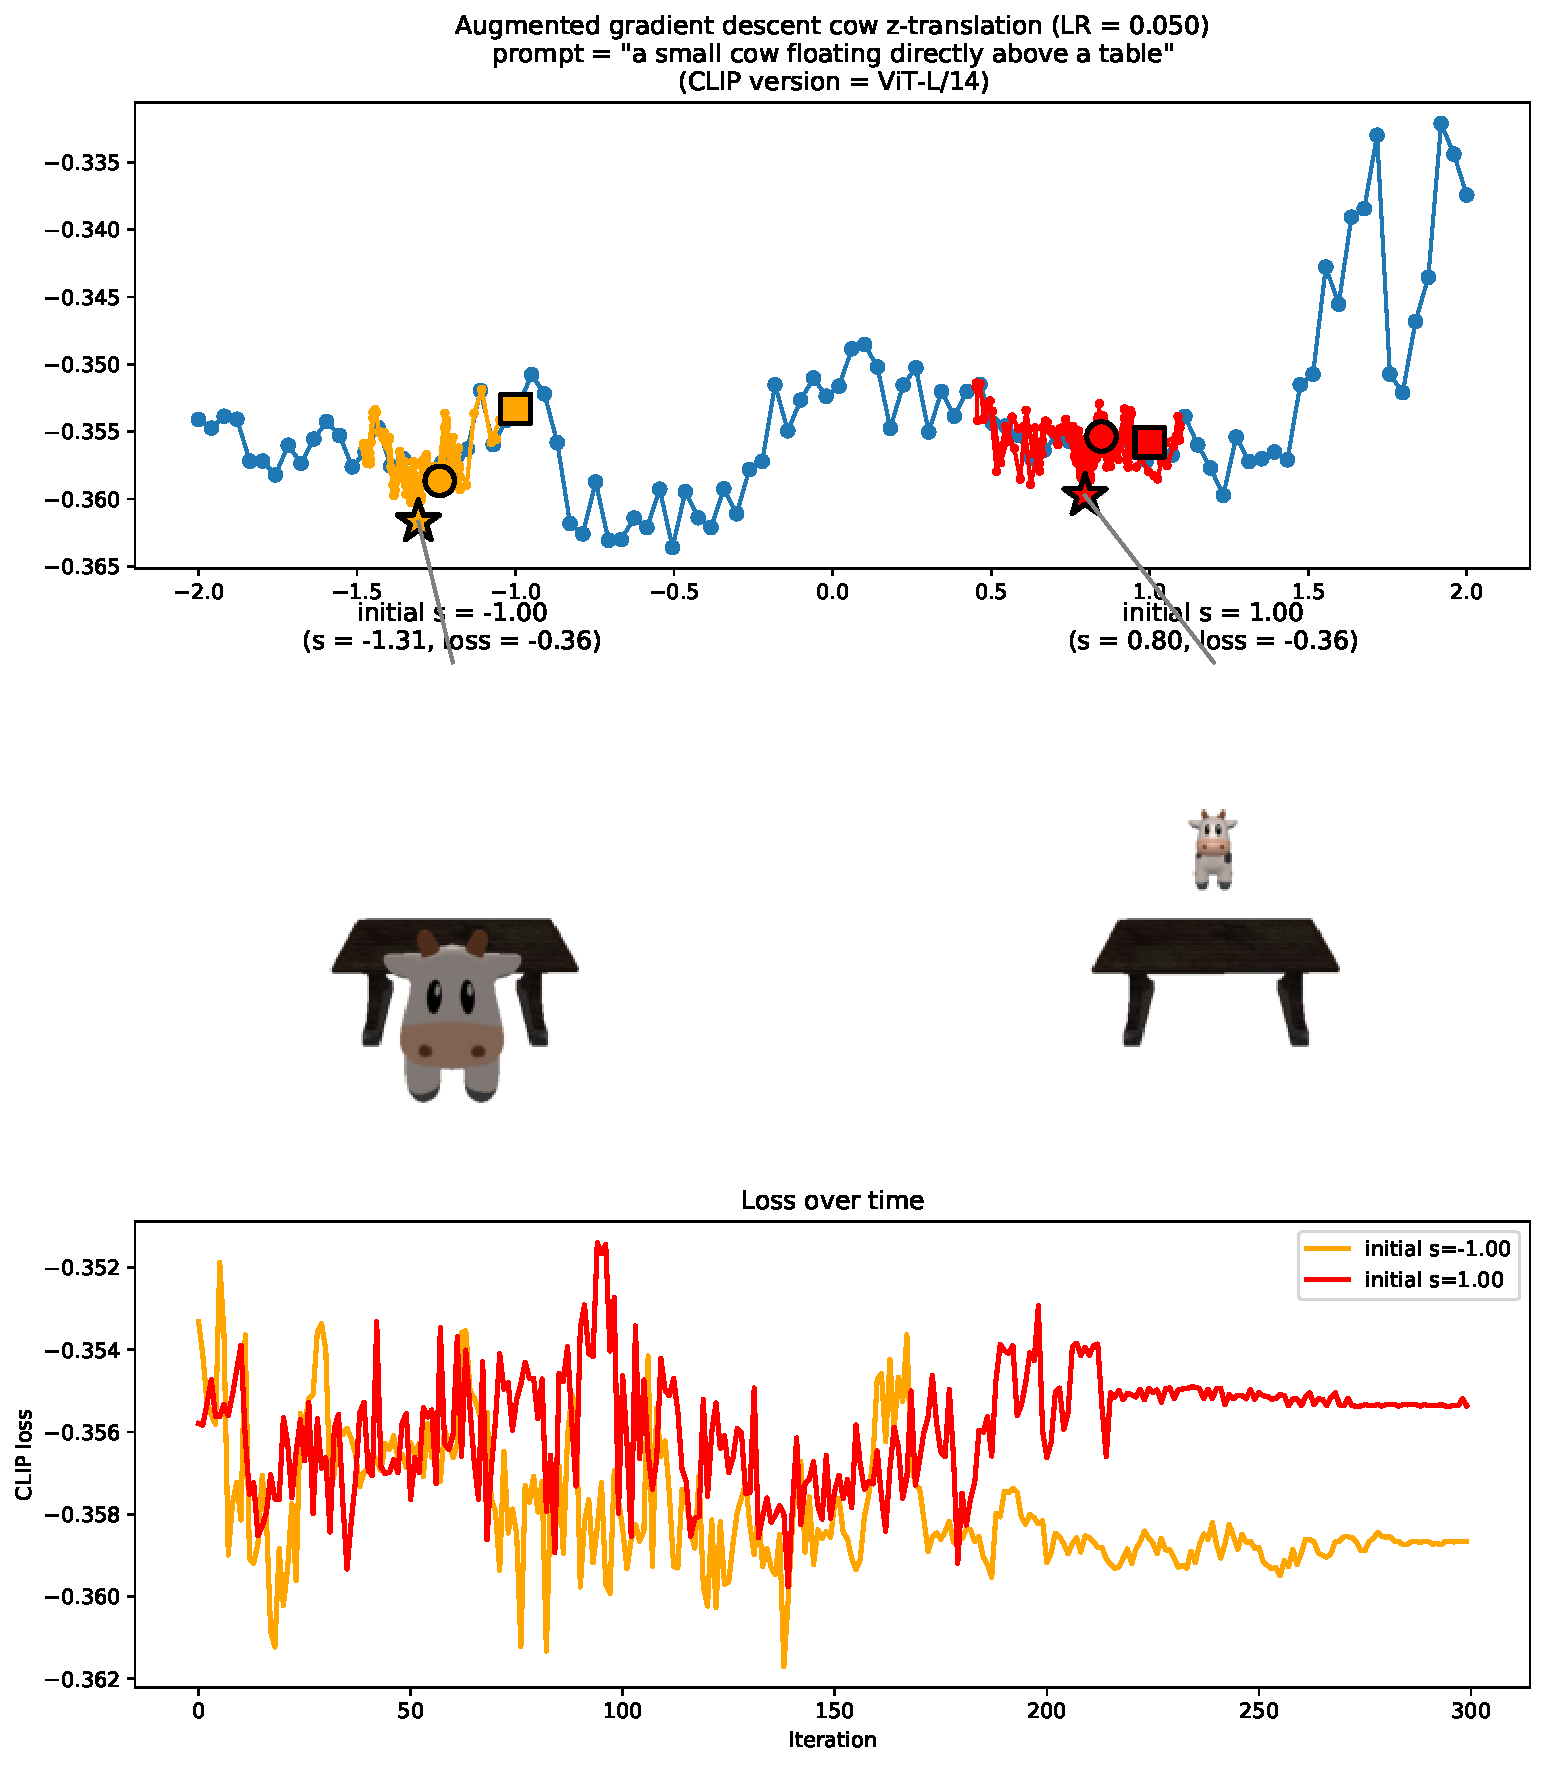
\includegraphics[width=1.0\textwidth]{figures/3_3-cow-aug-gd.pdf}
    \caption{Augmented gradient descent for cow z-translation. Top row shows the loss landscape overlaid with the two gradient descent paths (square denotes starting point, circle denotes final iteration, star denotes lowest loss encountered). Middle row shows the produced images for the encountered minima. Bottom row shows the learning curve (i.e. loss over time) for the two runs.}
    \label{fig:3_3-cow-aug-gd}
\end{figure}

Figure \ref{fig:3_3-cow-aug-gd} shows that the loss landscape has changed quite drastically compared to the non-augmented results in fig \ref{figs:3_3-cow-vanilla-gd}. The minimum is no longer located around $s=1.5$, but has instead shifted towards $s=-0.5$. This isn't exactly $s=0$, but it's a step in the right direction.  As for the quality of the gradient descent solutions, not much has improved. Neither of the two starting points end up yielding a solution near the global minimum. In fact, the loss over time (i.e. training curve) appears seems a bit more noisy this time.


% multiparam intro
Now it's time to introduce additional transformation parameters. Respectively, the new parameters are: [scale, x-rotation, y-rotation, z-rotation, x-translation, y-translation, z-translation]. Similar to the 2D example, all the parameters are "bounded" using the sigmoid function for scale, and $\tanh$ for all other parameters. Examples of rendered images using various parameters can be seen in figure \ref{fig:3_3-example-images}.

% multiparam - no augment
The problem can effectively be treated the same as the 2D multiparameter mug renderer from the previous subchapter, where instead of 4 parameters, there is now 7 in total. A training loop was set up for 300 iterations with Adam, initial LR = 0.01, a cosine annealing learning rate scheduler, and the starting point $\textbf{s} = \textbf{0}$. The novel view augmentation technique is \textit{not} included for this experiment. The results can be seen in figure \ref{fig:3_3-loss-graph}.
\begin{figure}[H]
    \centering
    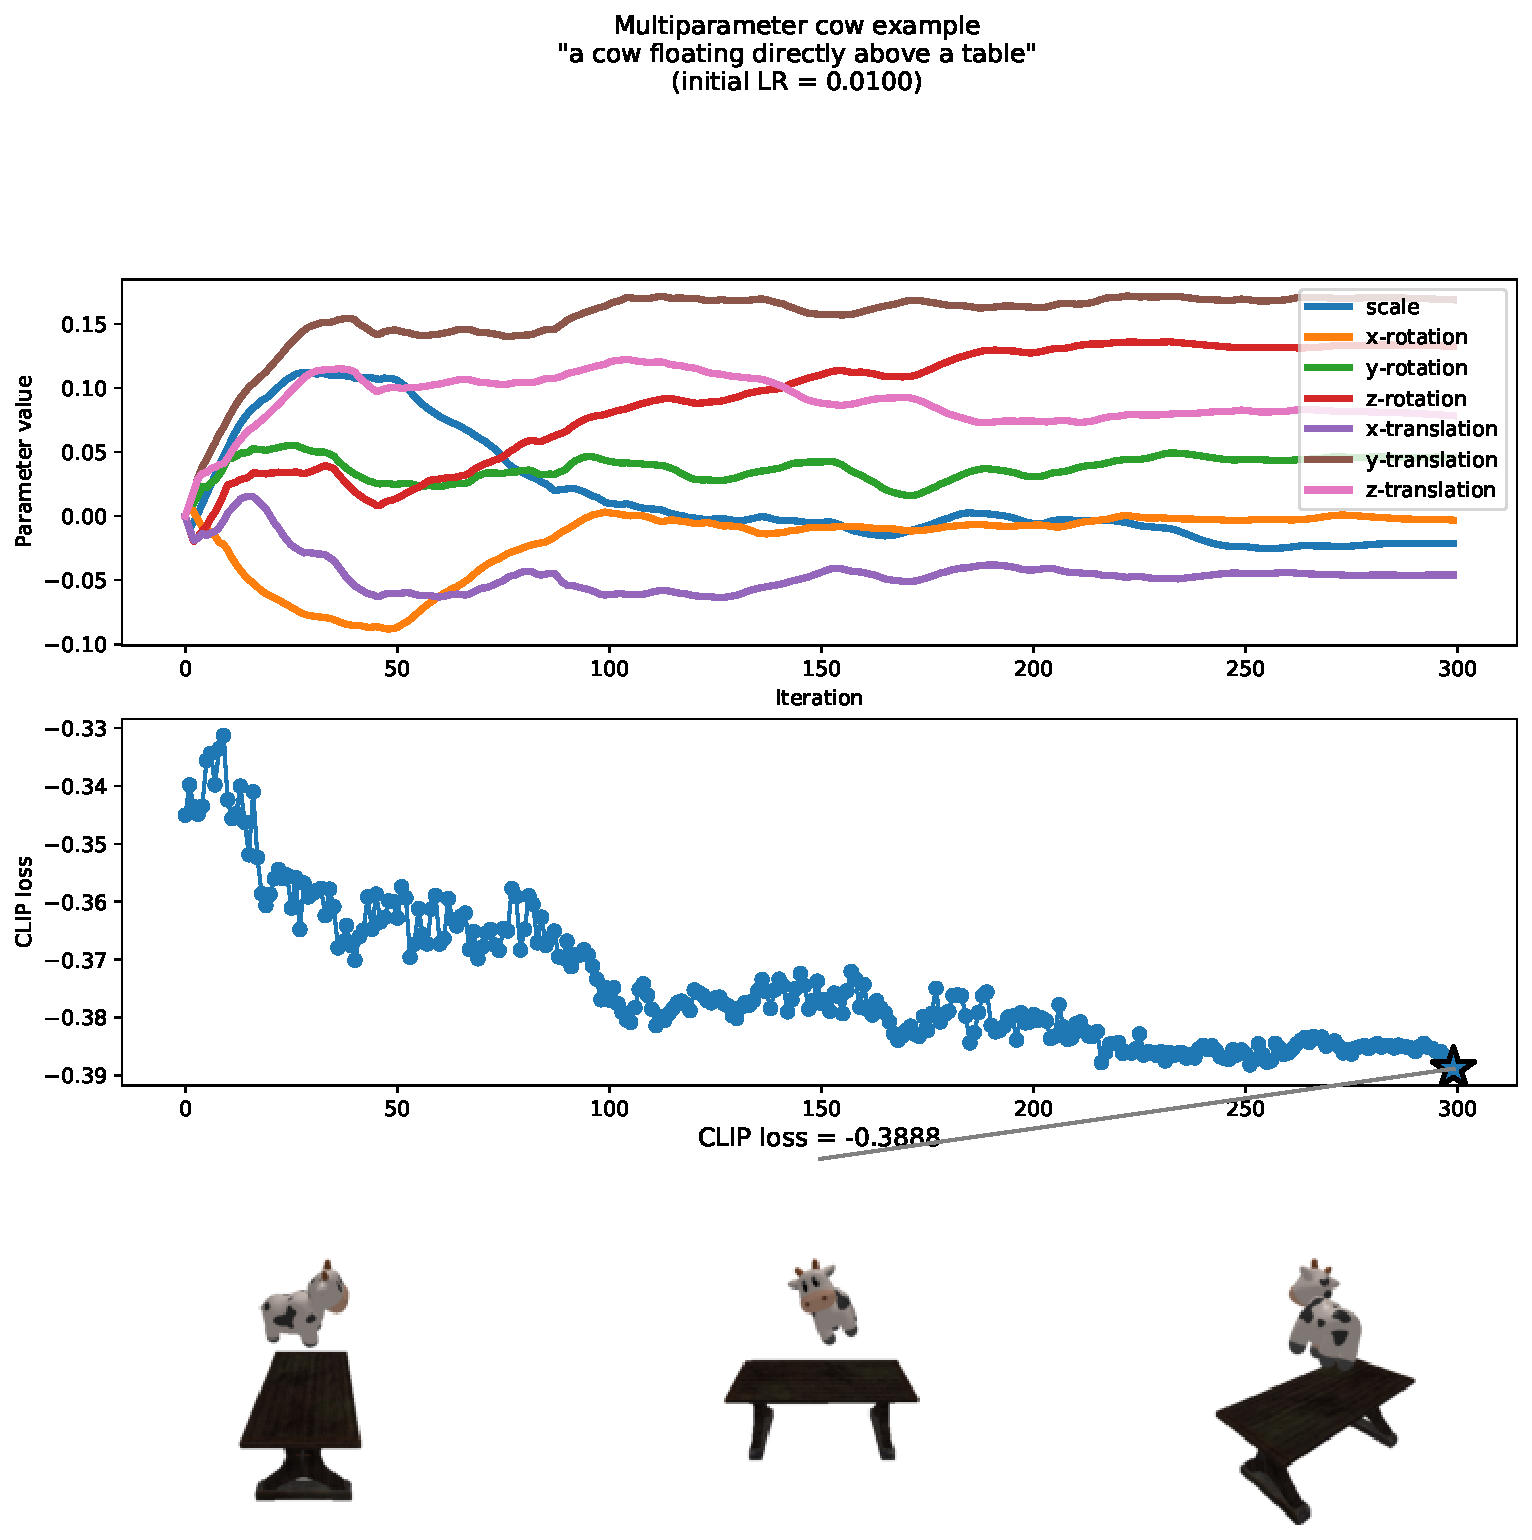
\includegraphics[width=1.0\textwidth]{figures/3_3-loss-graph.pdf}
    \caption{Non-augmented gradient descent for the multiparameter cow renderer. Top row shows how the transformation parameter evolve over time. Middle row shows how the CLIP loss evolves over time. Bottom row shows three rendered perspectives of the optimal solution.}
    \label{fig:3_3-loss-graph}
\end{figure}
Figure \ref{fig:3_3-loss-graph} shows that the loss seems to converge to a minimum over time. Also, the values of the parameters $\textbf{s}$ appear to lie in the range of $[-0.10, 0.15]$. Despite their magnitude, these small parameter values are apparently capable of reducing the loss from the initial $-0.345$ to about $-0.39$. Also, the fact that the y-translation parameter goes from $0$ to a bit over $0.15$ is interesting, since this is what actually makes the cow float above the table. It also seems to slightly rotate the cow.


% multiparam - augment
For the next experiment, the same training loop for the multiparameter cow renderer is used. However, this time, the novel view augmentations are added. This produced the results seen in figure \ref{fig:3_3-loss-graph-aug}

\begin{figure}[H]
    \centering
    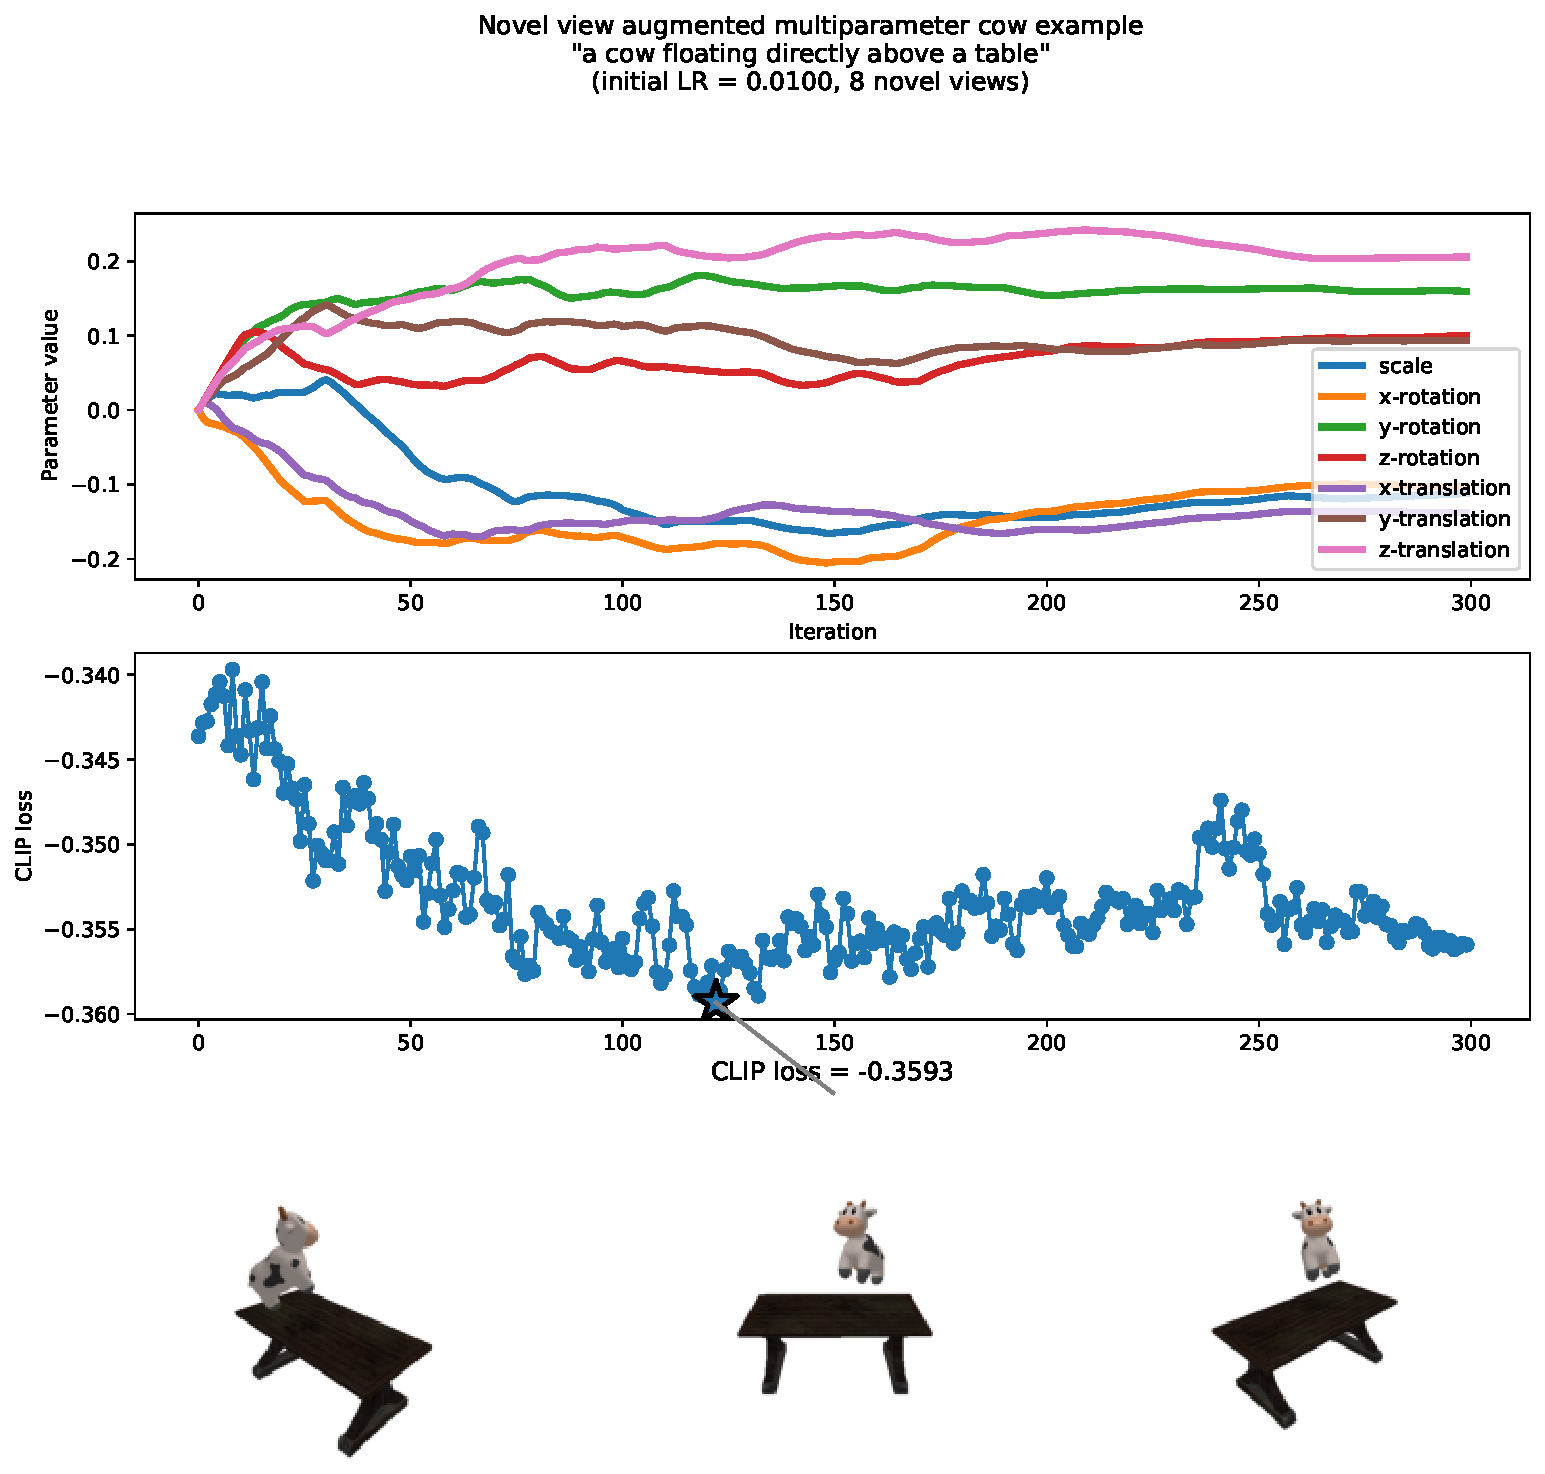
\includegraphics[width=1.0\textwidth]{figures/3_3-loss-graph-aug.pdf}
    \caption{Novel view augmented gradient descent for the multiparameter cow renderer. Top row shows how the transformation parameter evolve over time. Middle row shows how the CLIP loss evolves over time. Bottom row shows three rendered perspectives of the optimal solution.}
    \label{fig:3_3-loss-graph-aug}
\end{figure}
Figure \ref{fig:3_3-loss-graph-aug} shows that the transformation still puts the cow slightly above the table (i.e. increases y-translation). The loss does not seem to converge as nicely as in the previous experiment. The cow seems to be translated to the side of the table, and, again, is slightly rotated. Thus, it's hard to say that the novel view augmentations improved things much for the multiparameter cow renderer.

% brute force
Recall the brute force example from the previous subchapter. The search space consisted of $20^4 = 160.000$ parameter combinations, which took just under 2 hours to search through. Since we now have 7 parameters, a grid of the same resolution would result in $20^7 = 1.280.000.000$ combinations, which, by extrapolation, would take around $16.000$ hours to search through. Considering the fact that brute force searching a grid of similar granularity is pretty much computationally infeasible, a brute force experiment was not carried out.

% subchapter recap
To summarize the findings of this subchapter:
\begin{itemize}[noitemsep]
    \item When performing manipulations in 3D, sometimes rendered images from additional perspectives are required in order to gain more visual information of the effect of the manipulation (see figure \ref{fig:3_3-cow-perspectives}).
    
    \item Novel view augmentation had the effect of drastically changing the shape of the loss landscape. When applying the novel view augmentations to the multiparameter cow example, it did not seem to have a significantly positive impact.
    
    \item Even though the image and text embeddings are very similar for the cow renderer example (i.e. losses of almost $-0.40$), it's still difficult for gradient descent to reach the global minimum.
\end{itemize}


\section{Disentangled NeRFs}
% disentangled nerf intro
Neural Radiance Fields (NeRFs) are capable of rendering photorealistic images from arbitrary perspectives. An essential part of the full pipeline is being able to sufficiently disentangle a foreground object from a NeRF scene. This is where \cite{benaim2022} will be applied. Once this disentanglement has been obtained, it becomes possible to perform 3D manipulations on the foreground object before re-inserting the object into the original scene.

% faster nerfs
At the beginning of the project, a lot of effort was put into finding a faster way to train new NeRFs. Traditionally, the training time is $\approx 12$ hours for a single scene, and the training has to be done twice per scene (once masked, once unmasked).

% office example
After trying out a couple of different implementations, a fork was made of \url{https://github.com/ashawkey/torch-ngp}, which is based on \cite{mueller2022}. It is written in PyTorch with bindings to some CUDA kernels. The goal was to modify the code to replicate the example from \cite{benaim2022} which disentangles the TV from the back wall of the office. To this end, two NeRFs were trained (with/without masking the TV). The results from training can be seen in figure \ref{fig:3_4-room-learning-curves}.
\begin{figure}[H]
    \centering
    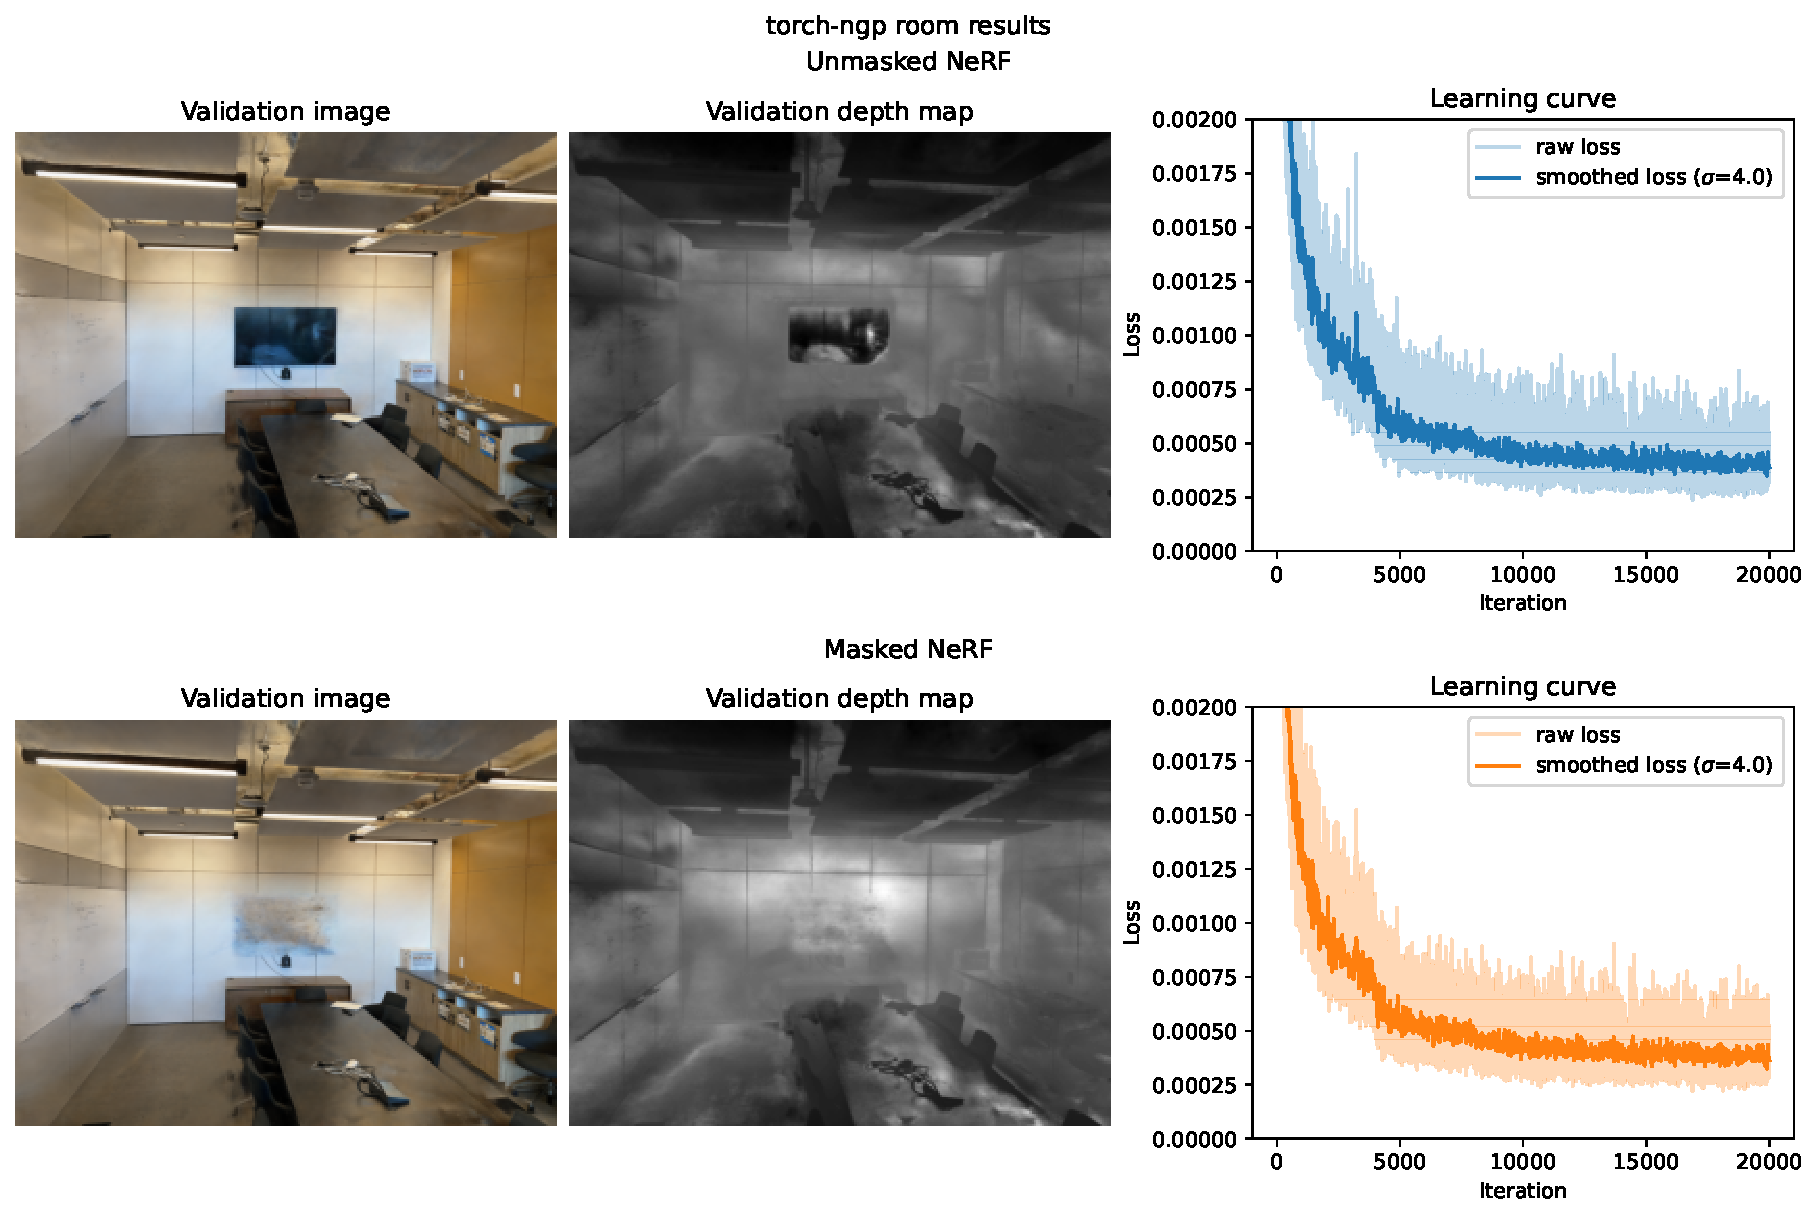
\includegraphics[width=1.0\textwidth]{figures/3_4-room-learning-curves.pdf}
    \caption{Results from training two NeRFs. Top row shows results from the unmasked example. Bottom row shows results from the masked example. First column shows an image rendered for a validation pose (i.e. not seen in the training data). Second column shows the associated depth map generated for the same validation pose. The last row shows the learning curves obtained from the training process.}
    \label{fig:3_4-room-learning-curves}
\end{figure}

Figure \ref{fig:3_4-room-learning-curves} shows that the loss curves have somewhat converged after 20k iterations. However, the depth maps are not looking very clear considering what a traditional NeRF is usually capable of producing.
Disregarding the noisy depth maps for now, a couple of disentanglement operations were performed for the two NeRFs. The first operation should only show the disentangled foreground object. The second operation should re-insert the disentangled foreground object into the background scene. The results can be seen in figure \ref{fig:3_4-room-disentanglement}.
\begin{figure}[H]
    \centering
    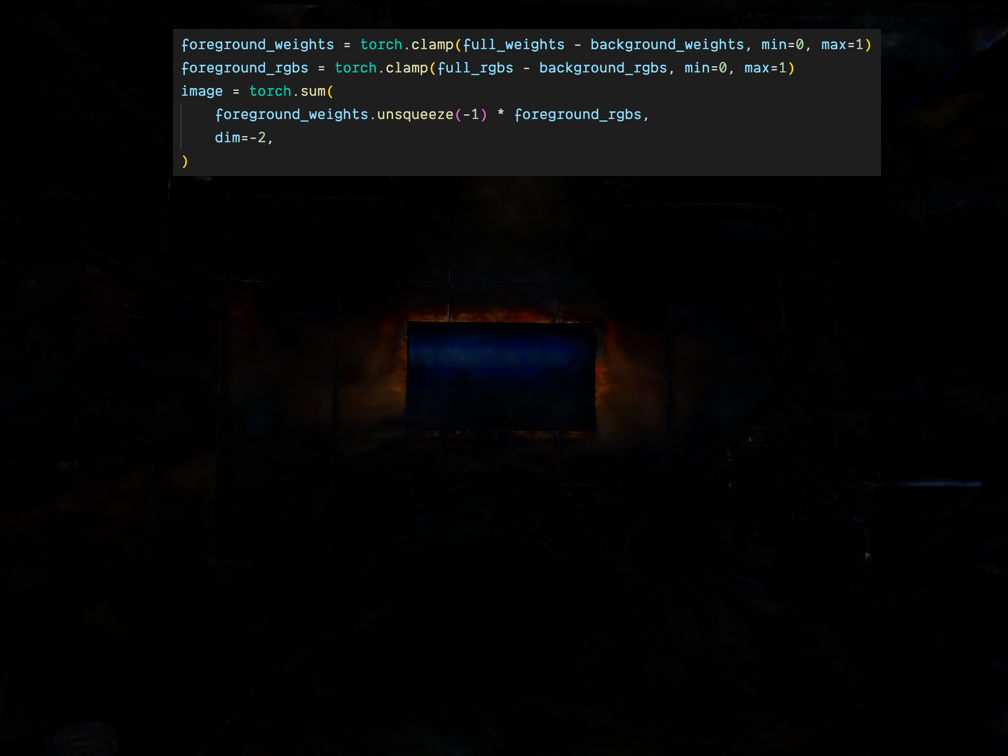
\includegraphics[width=1.0\textwidth]{figures/3_4-room-fg.png}
    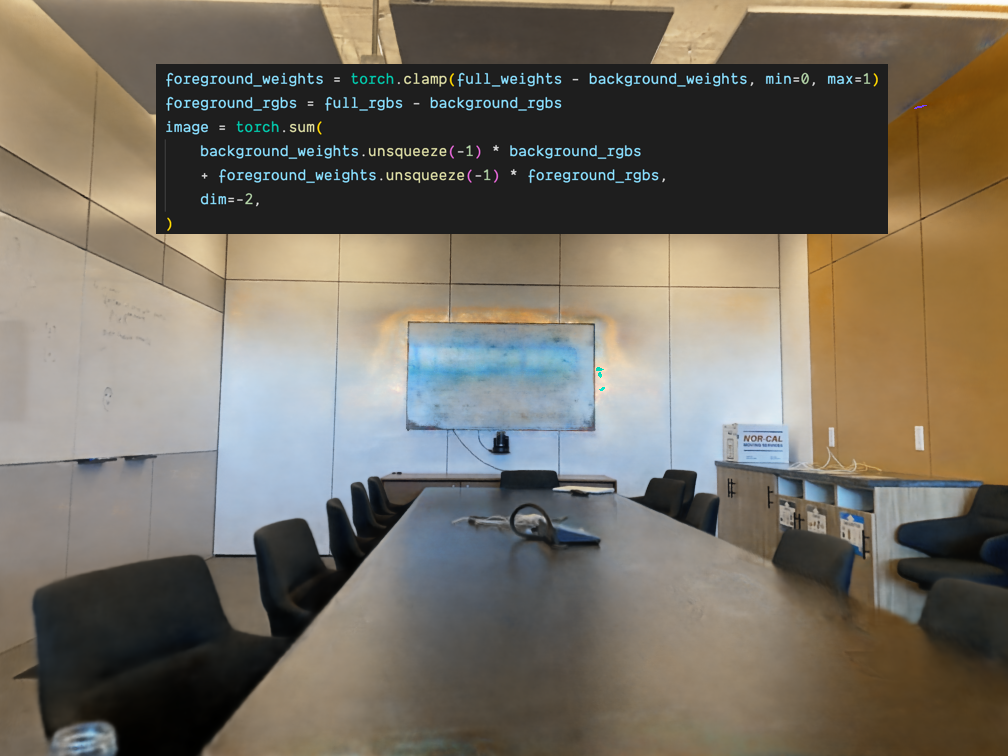
\includegraphics[width=1.0\textwidth]{figures/3_4-room-recombined-no-rgbclamp.png}

    \caption{TV disentanglement results. The exact equation used (in code form) for making each image is shown at the top.}
    \label{fig:3_4-room-disentanglement}
\end{figure}

Figure \ref{fig:3_4-room-disentanglement} shows some rather underwhelming results for the disentanglement operations. It was a bit unclear why this was happening - below is a list of suspected reasons:
\begin{itemize}[noitemsep]
    \item Code error (pretty likely, considering the fact that an entirely different codebase is used)
    \item Scenes weren't trained for long enough (poor depth maps could be a symptom of this)
    \item Too many collisions are happening with the multiresolution hash encoding, which makes disentanglement difficult (again, poor depth maps could be a symptom of this)
\end{itemize}

% flower example
Instead of going too far down the debugging rabbit hole, a different set of pre-trained vanilla NeRFs was obtained. These NeRFs were trained on images of a red flower. The results from training these vanilla NeRFs can be seen in figure \ref{fig:3_4-flower-learning-curves}.

\begin{figure}[H]
    \centering
    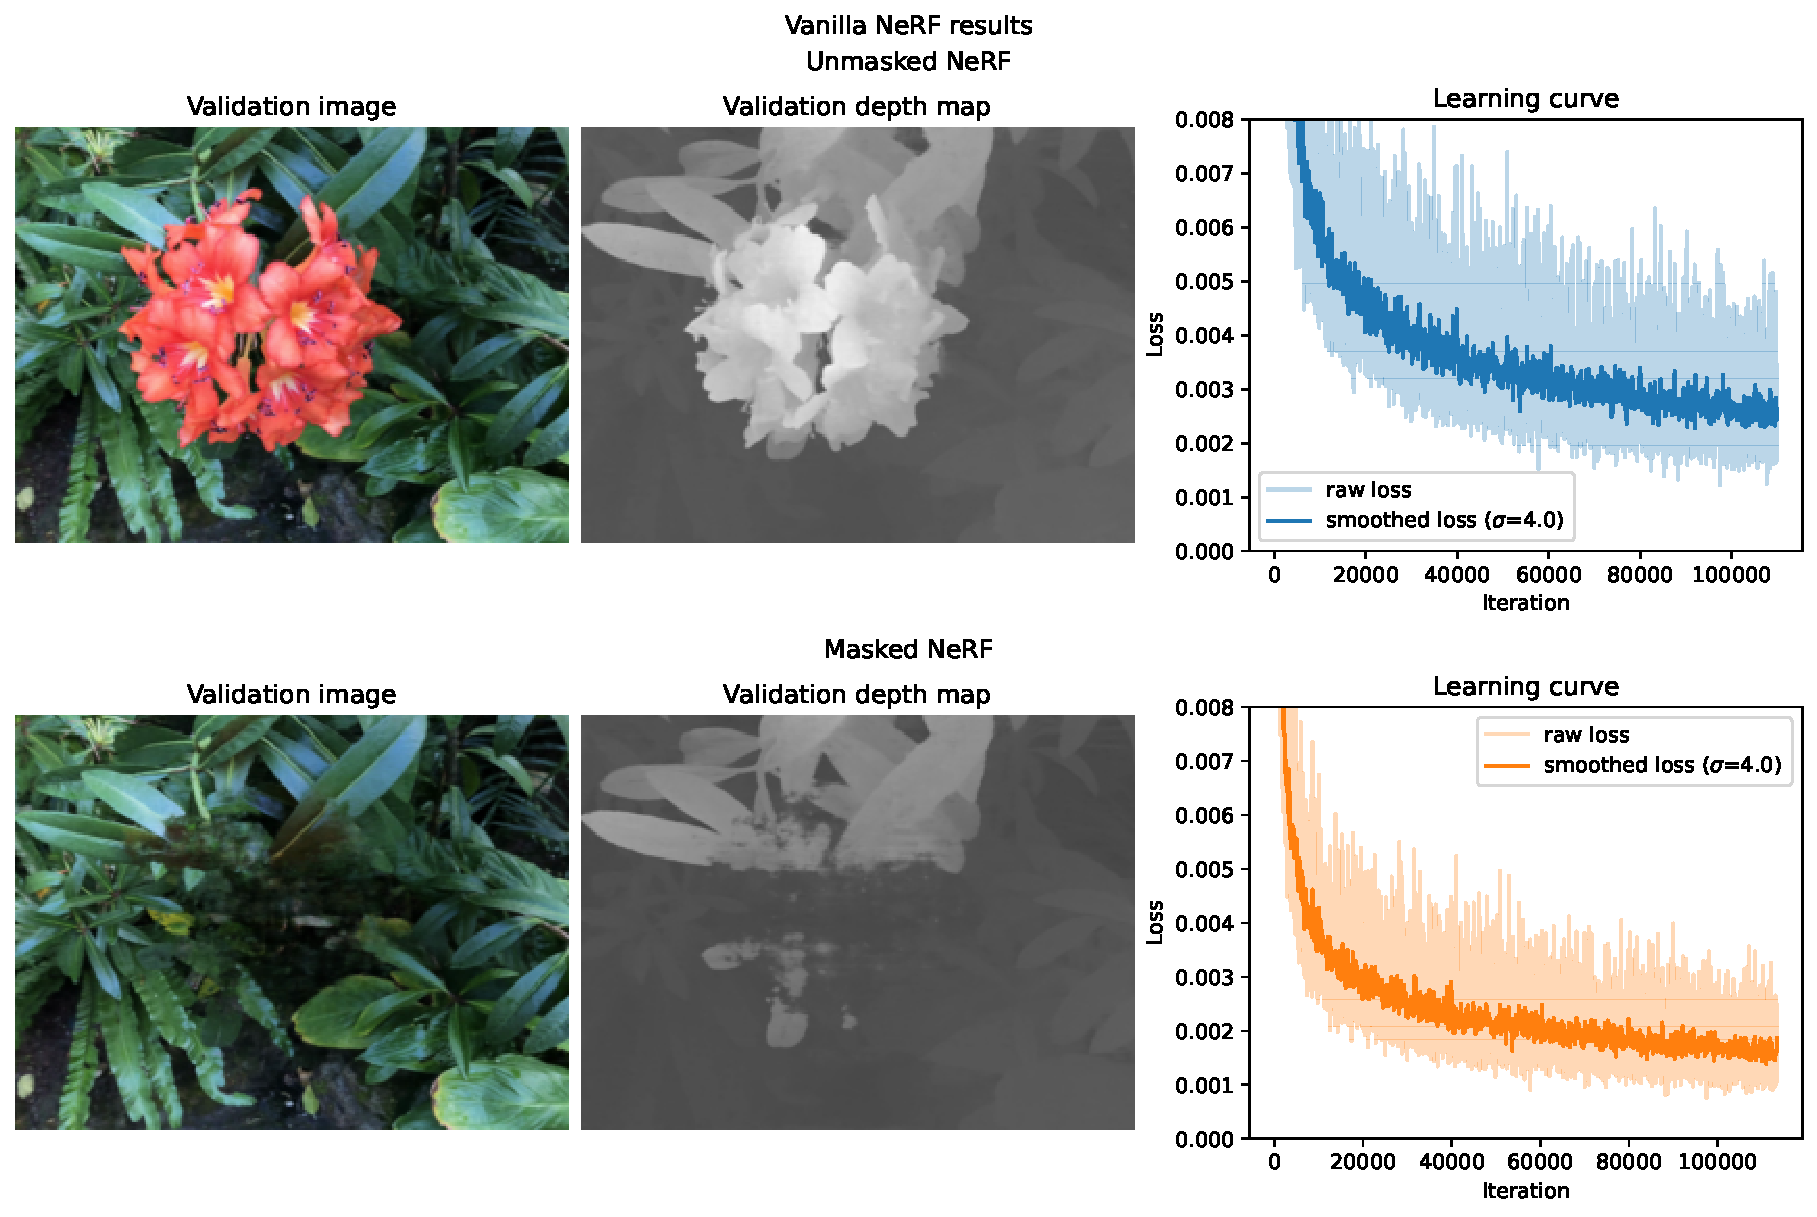
\includegraphics[width=1.0\textwidth]{figures/3_4-flower-learning-curves.pdf}
    \caption{Results from training two vanilla NeRFs. Top row shows results from the unmasked example. Bottom row shows results from the masked example. First column shows an image rendered for a validation pose (i.e. not seen in the training data). Second column shows the associated depth map generated for the same validation pose. The last row shows the learning curves obtained from the training process.}
    \label{fig:3_4-flower-learning-curves}
\end{figure}

Figure \ref{fig:3_4-flower-learning-curves} shows much clearer depth maps compared to those seen in figure \ref{fig:3_4-room-learning-curves}. The learning curves seem to be a bit more noisy this time, as well - in fact, it seems that the previous learning curves were a bit more stable towards the end.


The same two disentanglement operations were performed for the flower example - i.e. first operation only shows the disentangled object, and the second operation shows the foreground object re-inserted into the background scene. The results can be seen in figure \ref{fig:3_4-flower-disentanglement}.
\begin{figure}[H]
    \centering
    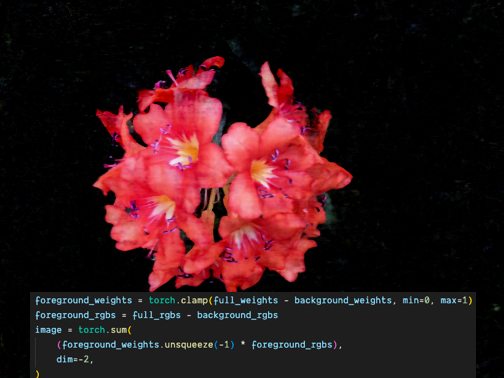
\includegraphics[width=1.0\textwidth]{figures/3_4-flower-fg.png}
    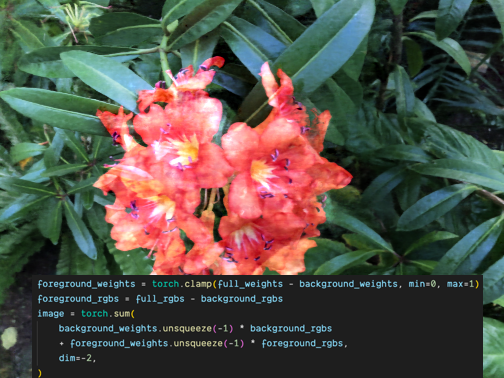
\includegraphics[width=1.0\textwidth]{figures/3_4-flower-recombined-no-rgbclamp.png}

    \caption{Flower disentanglement results. The exact equation used (in code form) for making each image is shown at the top.}
    \label{fig:3_4-flower-disentanglement}
\end{figure}

The results from figure \ref{fig:3_4-flower-disentanglement} are significantly better than those obtained for the TV disentanglement. However, some visual artifacts can still be observed - especially for the re-insertion example on the bottom row. The flower becomes a bit "translucent" in its appearance, as if it has lost some of its density.

The exact reason behind the artifacts was never quite understood. Trying different formulas for the disentanglement (e.g. adding/removing clamp operations, adding expanded terms, etc.) did not improve the results either. Again, instead of going too far down the debugging rabbit hole, the artifacts were ignored in order to continue with the transformations.

% transformations
The methodology for disentangled NeRF manipulations (described in section \ref{sec:nerf-manipulation}) can now be applied to the disentangled flower. This produced the results seen in figure \ref{fig:3_4-flower-transformations-successful}.

% successful flower transformations
\begin{figure}[H]
    \centering
    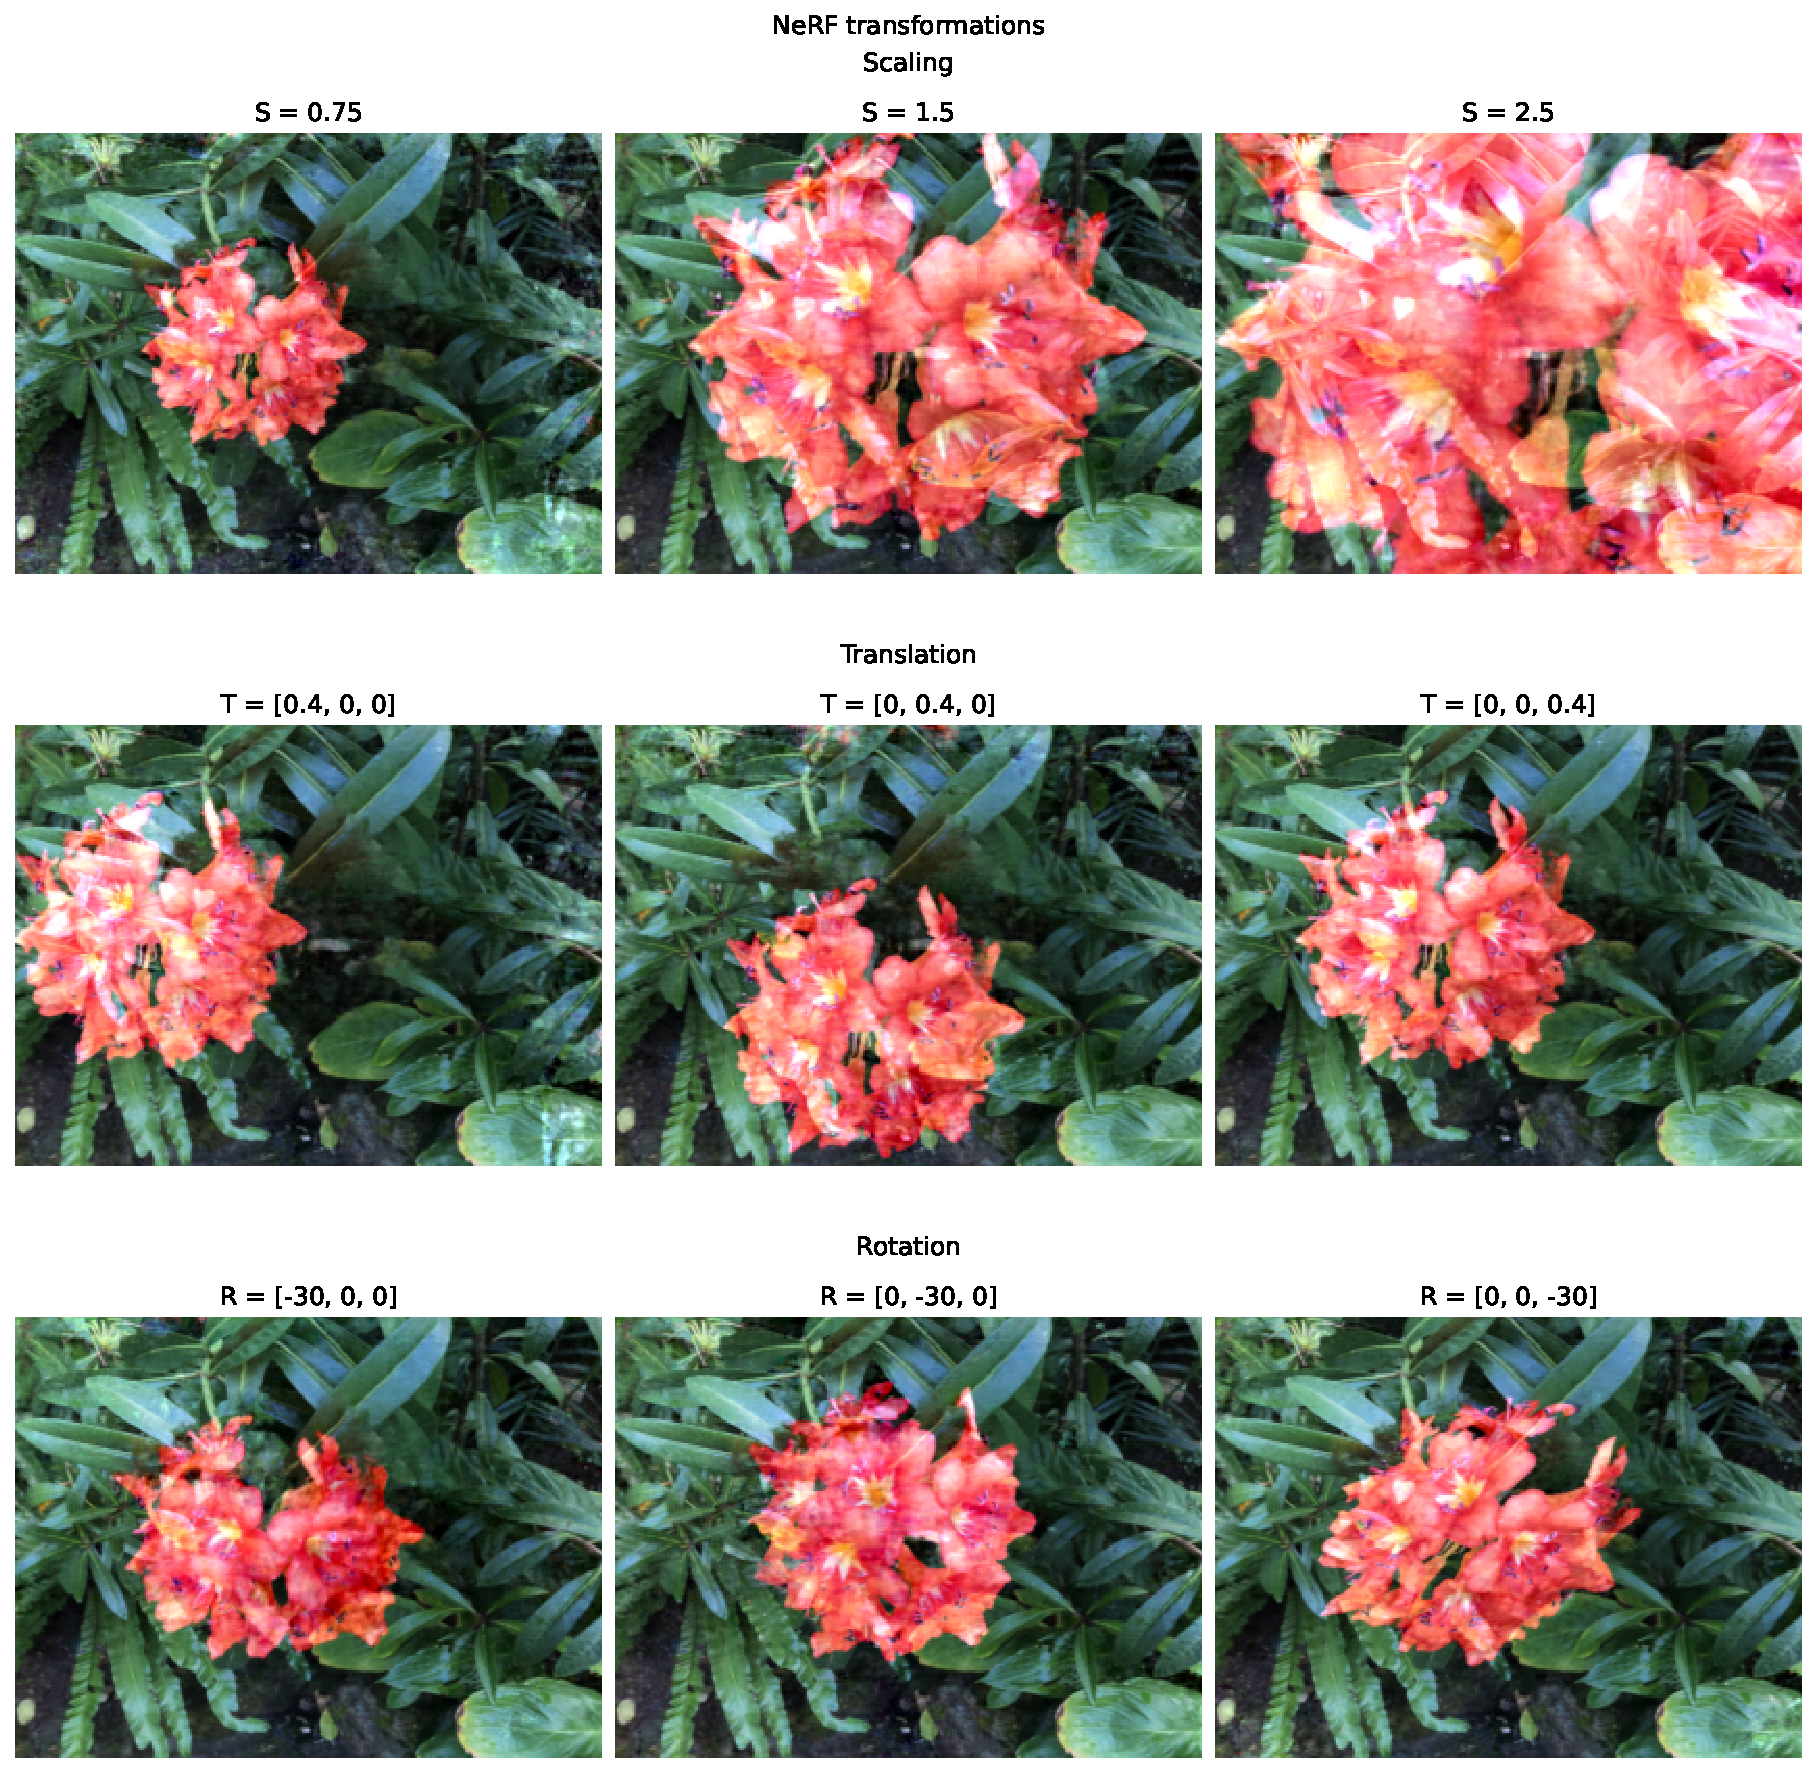
\includegraphics[width=1.0\textwidth]{figures/3_4-flower-transformations-successful.pdf}
    \caption{Flower transformations. First row shows scaling operations. Second row shows translation operations stated as [x,y,z]. Third row shows rotation operations stated as [x,y,z] (in degrees)}
    \label{fig:3_4-flower-transformations-successful}
\end{figure}
Figure \ref{fig:3_4-flower-transformations-successful} shows that the transformation parameters work to a certain extent. It seems to be possible to manipulate the foreground object while keeping the background intact. There is some visible noise that can be seen on the background - the intensity of which depends on the extent of the manipulation. Also, the z-rotation seems to skew the flower, which is not ideal.

% failed flower transformations
However, there is a limit to how much the foreground object can be transformed without starting to degenerate. This is due to the fact that NeRFs are only able to interpolate, and are unable to extrapolate to wildly unseen perspectives - i.e. NeRFs are "bounded" to the given input views, and trying to escape these bounds will yield weird images. Trying a wider range of transformation parameters produced the results seen in figure \ref{fig:3_4-flower-transformations-failed}.
\begin{figure}[H]
    \centering
    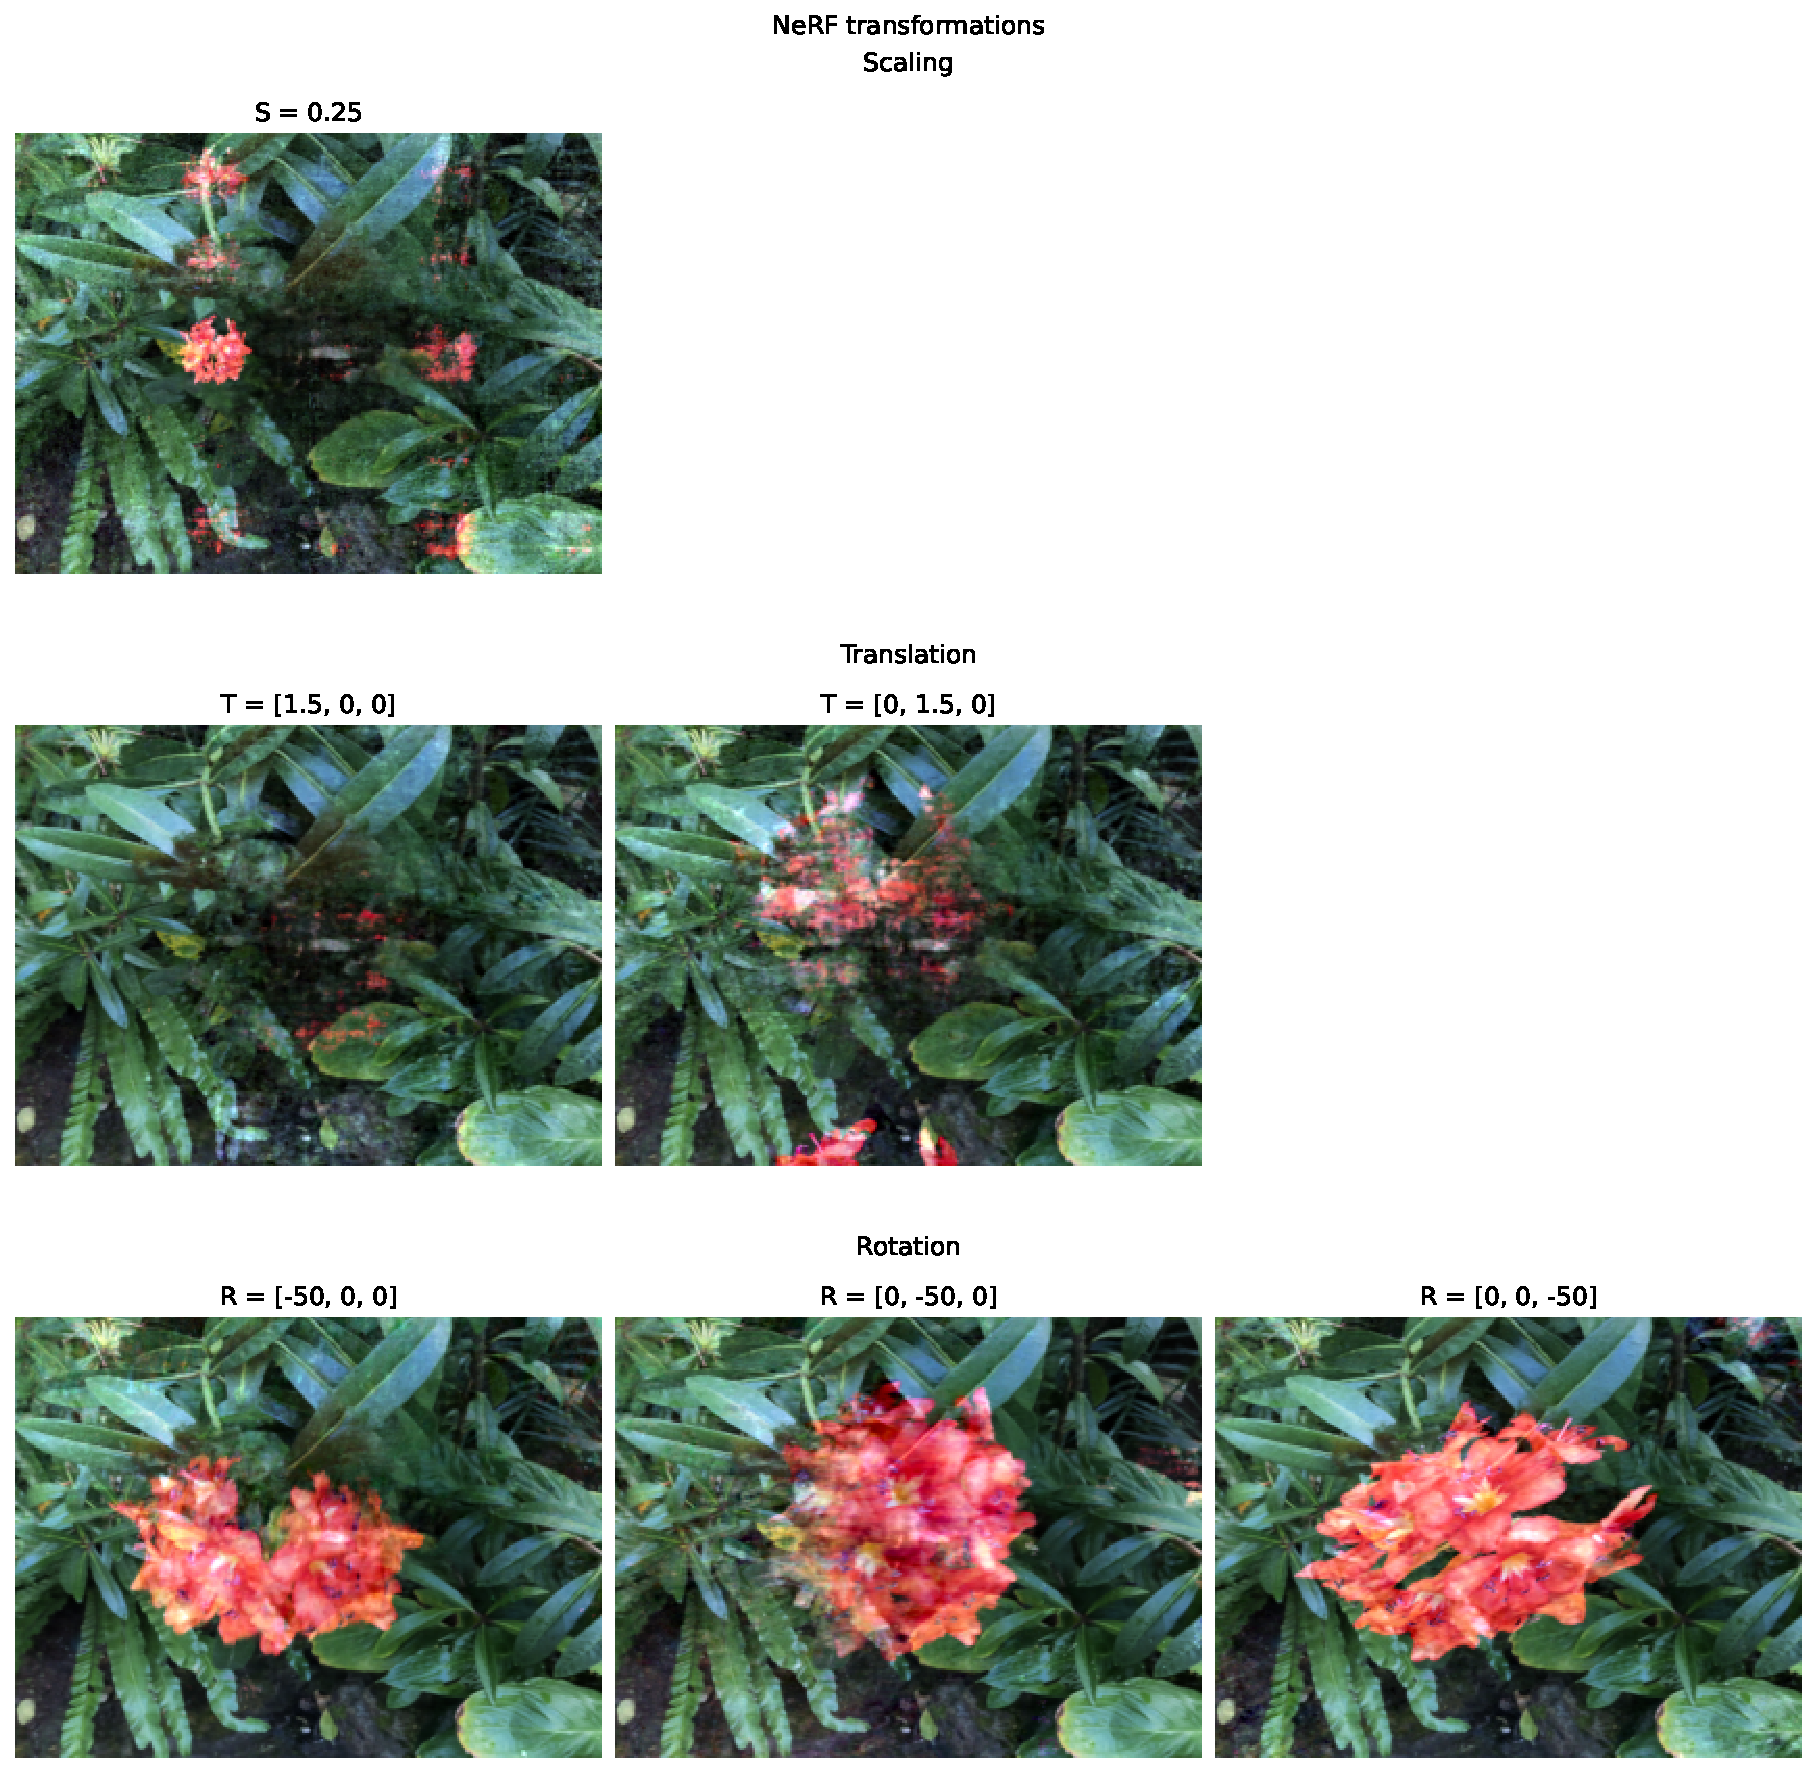
\includegraphics[width=1.0\textwidth]{figures/3_4-flower-transformations-failed.pdf}
    \caption{Flower transformations. First row shows scaling operations. Second row shows translation operations stated as [x,y,z]. Third row shows rotation operations stated as [x,y,z] (and in degrees)}
    \label{fig:3_4-flower-transformations-failed}
\end{figure}
The first row in figure \ref{fig:3_4-flower-transformations-failed} shows a type of "mosaic" visual artifacts appearing when the flower scale becomes very small. This could likely be the same artifact observed in the extreme translations in the second row. The third row shows that the flower starts disappearing for extreme rotations about x and y. However, the extreme z-translation does not appear to exhibit the same type of artifact.

% subchapter recap
\begin{itemize}[noitemsep]
    \item Using the \textit{torch-ngp} implementation (i.e. multiresolution hash encoding) of NeRF wasn't immediately well-suited for disentangled NeRFs. The reason behind this is a bit unclear and requires further debugging.

    \item Using vanilla NeRFs, it appears to be possible to perform transformations in 3D space - within the limitations imposed by the NeRFs.
    
    \item There are still a few issues with the implementation that need to be resolved - e.g. the "translucency" visual artifact, and the skewed z-rotation.
\end{itemize}
